\documentclass[11pt]{article}

% ---------------------------------------------------------------------------
% Preamble
% ---------------------------------------------------------------------------
\usepackage[T1]{fontenc}
\usepackage[utf8]{inputenc}
\usepackage{lmodern}
\usepackage[margin=1in]{geometry}
\usepackage{microtype}
\usepackage{amsmath,amssymb}
\usepackage{graphicx}
\usepackage{booktabs}
\usepackage{multirow}
\usepackage{array}
\usepackage{longtable}
\usepackage{xcolor}
\usepackage{enumitem}
\usepackage[font=small,labelfont=bf]{caption}
\usepackage[round,authoryear]{natbib}
\usepackage[colorlinks=true,linkcolor=blue!60!black,citecolor=blue!60!black,urlcolor=blue!60!black]{hyperref}
\usepackage[nameinlink,capitalize]{cleveref}

% Keep figures and tables near the paragraph that discusses them: every float is
% geared [tbp] and a \FloatBarrier fires at each \section, so no figure can drift
% past its section (or past the bibliography).
\usepackage[section]{placeins}
\emergencystretch=2em                % avoid 10-20 pt overfull lines without changing the wording
\renewcommand{\topfraction}{0.92}
\renewcommand{\bottomfraction}{0.55}
\renewcommand{\textfraction}{0.05}
\renewcommand{\floatpagefraction}{0.88}
\setcounter{topnumber}{3}
\setcounter{bottomnumber}{2}
\setcounter{totalnumber}{5}
\setlength{\floatsep}{10pt plus 2pt}
\setlength{\textfloatsep}{12pt plus 3pt}

\graphicspath{{figures/pdf/}}

% Pending-result marker: every unfilled number in the draft is explicit.
\newcommand{\todo}[1]{\textcolor{red}{\textbf{[#1]}}}
% System name used throughout.
\newcommand{\sys}{\textsc{thermo-agent}}
% Measured numbers: one macro per value, defined in generated/values.tex from assets_summary.json.
\expandafter\def\csname val@aud.ex_fuel_mw\endcsname{127}
\expandafter\def\csname val@aud.ex_pm_ed_mw\endcsname{41.7}
\expandafter\def\csname val@aud.ex_pm_energy_mw\endcsname{1.3}
\expandafter\def\csname val@aud.ex_pm_id\endcsname{\texttt{CC}}
\expandafter\def\csname val@aud.ex_rej_ed_mw\endcsname{2.5}
\expandafter\def\csname val@aud.ex_rej_energy_mw\endcsname{72.7}
\expandafter\def\csname val@aud.ex_rej_id\endcsname{\texttt{REJ}}
\expandafter\def\csname val@aud.ex_top_ed_mw\endcsname{17.0}
\expandafter\def\csname val@aud.ex_top_id\endcsname{\texttt{HX}}
\expandafter\def\csname val@aud.fl_ci_hi_id_pct\endcsname{4}
\expandafter\def\csname val@aud.fl_ci_hi_ood_pct\endcsname{100}
\expandafter\def\csname val@aud.fl_ci_lo_id_pct\endcsname{0}
\expandafter\def\csname val@aud.fl_ci_lo_ood_pct\endcsname{96}
\expandafter\def\csname val@aud.fl_hits_id\endcsname{0}
\expandafter\def\csname val@aud.fl_hits_ood\endcsname{100}
\expandafter\def\csname val@aud.fl_top1_id_pct\endcsname{0}
\expandafter\def\csname val@aud.fl_top1_ood_pct\endcsname{100}
\expandafter\def\csname val@aud.n_id\endcsname{100}
\expandafter\def\csname val@aud.n_ood\endcsname{100}
\expandafter\def\csname val@aud.ndcg_fl_id\endcsname{0.627}
\expandafter\def\csname val@aud.ndcg_fl_ood\endcsname{1.000}
\expandafter\def\csname val@aud.ndcg_rnd_id\endcsname{0.693}
\expandafter\def\csname val@aud.ndcg_rnd_ood\endcsname{0.865}
\expandafter\def\csname val@aud.rnd_top1_id_pct\endcsname{23}
\expandafter\def\csname val@aud.rnd_top1_ood_pct\endcsname{81}
\expandafter\def\csname val@audb.fl_top1_id_pct\endcsname{0}
\expandafter\def\csname val@audb.fl_top1_ood_pct\endcsname{100}
\expandafter\def\csname val@audb.n_id\endcsname{100}
\expandafter\def\csname val@audb.n_ood\endcsname{100}
\expandafter\def\csname val@audb.n_total\endcsname{200}
\expandafter\def\csname val@audb.pred_mean_id\endcsname{0.47}
\expandafter\def\csname val@audb.pred_mean_ood\endcsname{0.34}
\expandafter\def\csname val@audb.pred_zero_id\endcsname{0.04}
\expandafter\def\csname val@audb.pred_zero_ood\endcsname{0.22}
\expandafter\def\csname val@audb.rnd_top1_id_pct\endcsname{23}
\expandafter\def\csname val@audb.rnd_top1_ood_pct\endcsname{81}
\expandafter\def\csname val@audb.rule_gain_id_pct\endcsname{65}
\expandafter\def\csname val@audb.rule_gain_ood_pct\endcsname{23}
\expandafter\def\csname val@audb.rule_valid_id\endcsname{53}
\expandafter\def\csname val@audb.rule_valid_ood\endcsname{100}
\expandafter\def\csname val@audb.saving_max_all_pct\endcsname{5.8}
\expandafter\def\csname val@audb.saving_max_id_pct\endcsname{5.8}
\expandafter\def\csname val@audb.saving_max_ood_pct\endcsname{1.3}
\expandafter\def\csname val@audb.saving_median_all_pct\endcsname{0.4}
\expandafter\def\csname val@audb.saving_median_id_pct\endcsname{1.7}
\expandafter\def\csname val@audb.saving_median_ood_pct\endcsname{0.2}
\expandafter\def\csname val@audb.saving_min_all_pct\endcsname{0.07}
\expandafter\def\csname val@audb.saving_min_id_pct\endcsname{0.07}
\expandafter\def\csname val@audb.saving_min_ood_pct\endcsname{0.07}
\expandafter\def\csname val@audb.search_evals_id\endcsname{12}
\expandafter\def\csname val@audb.search_evals_ood\endcsname{8}
\expandafter\def\csname val@corp.arch_distinct.test_id\endcsname{37}
\expandafter\def\csname val@corp.arch_distinct.test_ood_fault\endcsname{44}
\expandafter\def\csname val@corp.arch_distinct.test_ood_topology\endcsname{8}
\expandafter\def\csname val@corp.arch_distinct.train\endcsname{45}
\expandafter\def\csname val@corp.arch_distinct.val\endcsname{39}
\expandafter\def\csname val@corp.arch_kept\endcsname{2{,}063}
\expandafter\def\csname val@corp.arch_kept_pct\endcsname{69}
\expandafter\def\csname val@corp.arch_requested\endcsname{3{,}000}
\expandafter\def\csname val@corp.arch_rows.test_id\endcsname{95}
\expandafter\def\csname val@corp.arch_rows.test_ood_fault\endcsname{761}
\expandafter\def\csname val@corp.arch_rows.test_ood_topology\endcsname{279}
\expandafter\def\csname val@corp.arch_rows.train\endcsname{818}
\expandafter\def\csname val@corp.arch_rows.val\endcsname{110}
\expandafter\def\csname val@corp.ground_min_pct\endcsname{80}
\expandafter\def\csname val@corp.harness_fraction\endcsname{35}
\expandafter\def\csname val@corp.k_memory\endcsname{3}
\expandafter\def\csname val@corp.max_prompt_chars\endcsname{11{,}500}
\expandafter\def\csname val@corp.max_prompt_tokens\endcsname{4{,}000}
\expandafter\def\csname val@corp.mem_min_score\endcsname{0.02}
\expandafter\def\csname val@corp.n_arch\endcsname{65}
\expandafter\def\csname val@corp.n_dc\endcsname{64}
\expandafter\def\csname val@corp.n_engine\endcsname{32}
\expandafter\def\csname val@corp.n_heat\endcsname{41}
\expandafter\def\csname val@corp.n_held\endcsname{9}
\expandafter\def\csname val@corp.n_orc\endcsname{33}
\expandafter\def\csname val@corp.n_turbine\endcsname{33}
\expandafter\def\csname val@corp.ndcg_min\endcsname{0.5}
\expandafter\def\csname val@corp.pred_err_max\endcsname{0.5}
\expandafter\def\csname val@corp.rows\endcsname{123{,}024}
\expandafter\def\csname val@corp.rows.audit.test_id\endcsname{321}
\expandafter\def\csname val@corp.rows.audit.test_ood_fault\endcsname{0}
\expandafter\def\csname val@corp.rows.audit.test_ood_topology\endcsname{238}
\expandafter\def\csname val@corp.rows.audit.train\endcsname{2{,}564}
\expandafter\def\csname val@corp.rows.audit.val\endcsname{338}
\expandafter\def\csname val@corp.rows.design.test_id\endcsname{204}
\expandafter\def\csname val@corp.rows.design.test_ood_climate\endcsname{615}
\expandafter\def\csname val@corp.rows.design.test_ood_load\endcsname{411}
\expandafter\def\csname val@corp.rows.design.test_ood_scale\endcsname{460}
\expandafter\def\csname val@corp.rows.design.train\endcsname{1{,}894}
\expandafter\def\csname val@corp.rows.design.val\endcsname{235}
\expandafter\def\csname val@corp.rows.ledger.test_id\endcsname{656}
\expandafter\def\csname val@corp.rows.ledger.test_ood_fault\endcsname{2{,}360}
\expandafter\def\csname val@corp.rows.ledger.test_ood_topology\endcsname{854}
\expandafter\def\csname val@corp.rows.ledger.train\endcsname{5{,}165}
\expandafter\def\csname val@corp.rows.ledger.val\endcsname{666}
\expandafter\def\csname val@corp.rows.repair.test_id\endcsname{563}
\expandafter\def\csname val@corp.rows.repair.test_ood_fault\endcsname{3{,}966}
\expandafter\def\csname val@corp.rows.repair.test_ood_topology\endcsname{864}
\expandafter\def\csname val@corp.rows.repair.train\endcsname{100{,}036}
\expandafter\def\csname val@corp.rows.repair.val\endcsname{614}
\expandafter\def\csname val@corp.rows_train\endcsname{109{,}659}
\expandafter\def\csname val@corp.samp_max_tokens\endcsname{800}
\expandafter\def\csname val@corp.samp_temperature\endcsname{0.8}
\expandafter\def\csname val@corp.var.efficiency_gt_1.max\endcsname{25}
\expandafter\def\csname val@corp.var.efficiency_gt_1.min\endcsname{25}
\expandafter\def\csname val@corp.var.unit_slip.max\endcsname{20}
\expandafter\def\csname val@corp.var.unit_slip.min\endcsname{20}
\expandafter\def\csname val@corp.var.wrong_fluid.max\endcsname{80}
\expandafter\def\csname val@corp.var.wrong_fluid.min\endcsname{80}
\expandafter\def\csname val@corp.var_max\endcsname{80}
\expandafter\def\csname val@corp.var_min\endcsname{20}
\expandafter\def\csname val@corp.variants_default\endcsname{20}
\expandafter\def\csname val@des.enum.b1.valid_pct\endcsname{88}
\expandafter\def\csname val@des.enum.b12.gap_pct\endcsname{13.1}
\expandafter\def\csname val@des.enum.b12.valid_pct\endcsname{96}
\expandafter\def\csname val@des.enum.b12.within_pct\endcsname{0}
\expandafter\def\csname val@des.enum.b128.gap_pct\endcsname{2.4}
\expandafter\def\csname val@des.enum.b128.valid_pct\endcsname{100}
\expandafter\def\csname val@des.enum.b128.within_pct\endcsname{71}
\expandafter\def\csname val@des.enum.b24.gap_pct\endcsname{8.2}
\expandafter\def\csname val@des.enum.b24.valid_pct\endcsname{100}
\expandafter\def\csname val@des.enum.b24.within_pct\endcsname{25}
\expandafter\def\csname val@des.enum.b32.gap_pct\endcsname{6.0}
\expandafter\def\csname val@des.enum.b32.valid_pct\endcsname{100}
\expandafter\def\csname val@des.enum.b32.within_pct\endcsname{33}
\expandafter\def\csname val@des.enum.b48.gap_pct\endcsname{4.3}
\expandafter\def\csname val@des.enum.b48.valid_pct\endcsname{100}
\expandafter\def\csname val@des.enum.b48.within_pct\endcsname{46}
\expandafter\def\csname val@des.enum.b64.gap_pct\endcsname{2.4}
\expandafter\def\csname val@des.enum.b64.valid_pct\endcsname{100}
\expandafter\def\csname val@des.enum.b64.within_pct\endcsname{71}
\expandafter\def\csname val@des.enum.b96.gap_pct\endcsname{2.4}
\expandafter\def\csname val@des.enum.b96.valid_pct\endcsname{100}
\expandafter\def\csname val@des.enum.b96.within_pct\endcsname{71}
\expandafter\def\csname val@des.enum_len_max\endcsname{64}
\expandafter\def\csname val@des.enum_len_min\endcsname{32}
\expandafter\def\csname val@des.n_heat_sites\endcsname{9}
\expandafter\def\csname val@des.n_sites\endcsname{24}
\expandafter\def\csname val@des.pol.b12.gap_pct\endcsname{13.1}
\expandafter\def\csname val@des.pol.b12.valid_pct\endcsname{96}
\expandafter\def\csname val@des.pol.b12.within_pct\endcsname{0}
\expandafter\def\csname val@des.pol.b128.gap_pct\endcsname{0.1}
\expandafter\def\csname val@des.pol.b128.valid_pct\endcsname{100}
\expandafter\def\csname val@des.pol.b128.within_pct\endcsname{100}
\expandafter\def\csname val@des.pol.b24.gap_pct\endcsname{8.2}
\expandafter\def\csname val@des.pol.b24.valid_pct\endcsname{100}
\expandafter\def\csname val@des.pol.b24.within_pct\endcsname{25}
\expandafter\def\csname val@des.pol.b32.gap_pct\endcsname{6.0}
\expandafter\def\csname val@des.pol.b32.valid_pct\endcsname{100}
\expandafter\def\csname val@des.pol.b32.within_pct\endcsname{33}
\expandafter\def\csname val@des.pol.b48.gap_pct\endcsname{3.7}
\expandafter\def\csname val@des.pol.b48.valid_pct\endcsname{100}
\expandafter\def\csname val@des.pol.b48.within_pct\endcsname{50}
\expandafter\def\csname val@des.pol.b64.gap_pct\endcsname{1.4}
\expandafter\def\csname val@des.pol.b64.valid_pct\endcsname{100}
\expandafter\def\csname val@des.pol.b64.within_pct\endcsname{79}
\expandafter\def\csname val@des.pol.b96.gap_pct\endcsname{0.3}
\expandafter\def\csname val@des.pol.b96.valid_pct\endcsname{100}
\expandafter\def\csname val@des.pol.b96.within_pct\endcsname{92}
\expandafter\def\csname val@des.polish_len_max\endcsname{144}
\expandafter\def\csname val@des.polish_len_min\endcsname{104}
\expandafter\def\csname val@des.rand.b1.valid_pct\endcsname{25}
\expandafter\def\csname val@des.rand.b12.gap_pct\endcsname{8.7}
\expandafter\def\csname val@des.rand.b12.valid_pct\endcsname{96}
\expandafter\def\csname val@des.rand.b12.within_pct\endcsname{33}
\expandafter\def\csname val@des.rand.b128.gap_pct\endcsname{0.6}
\expandafter\def\csname val@des.rand.b128.valid_pct\endcsname{100}
\expandafter\def\csname val@des.rand.b128.within_pct\endcsname{75}
\expandafter\def\csname val@des.rand.b24.gap_pct\endcsname{5.0}
\expandafter\def\csname val@des.rand.b24.valid_pct\endcsname{100}
\expandafter\def\csname val@des.rand.b24.within_pct\endcsname{42}
\expandafter\def\csname val@des.rand.b32.gap_pct\endcsname{3.6}
\expandafter\def\csname val@des.rand.b32.valid_pct\endcsname{100}
\expandafter\def\csname val@des.rand.b32.within_pct\endcsname{46}
\expandafter\def\csname val@des.rand.b48.gap_pct\endcsname{2.9}
\expandafter\def\csname val@des.rand.b48.valid_pct\endcsname{100}
\expandafter\def\csname val@des.rand.b48.within_pct\endcsname{54}
\expandafter\def\csname val@des.rand.b64.gap_pct\endcsname{1.6}
\expandafter\def\csname val@des.rand.b64.valid_pct\endcsname{100}
\expandafter\def\csname val@des.rand.b64.within_pct\endcsname{67}
\expandafter\def\csname val@des.rand.b96.gap_pct\endcsname{0.9}
\expandafter\def\csname val@des.rand.b96.valid_pct\endcsname{100}
\expandafter\def\csname val@des.rand.b96.within_pct\endcsname{71}
\expandafter\def\csname val@des.random_len\endcsname{130}
\expandafter\def\csname val@des.split.test_id\endcsname{5}
\expandafter\def\csname val@des.split.test_ood_climate\endcsname{11}
\expandafter\def\csname val@des.split.test_ood_load\endcsname{4}
\expandafter\def\csname val@des.split.test_ood_scale\endcsname{2}
\expandafter\def\csname val@des.split.val\endcsname{2}
\expandafter\def\csname val@des.tolerance_pct\endcsname{2}
\expandafter\def\csname val@env.n_catalog\endcsname{32}
\expandafter\def\csname val@env.n_catalog_heat\endcsname{64}
\expandafter\def\csname val@env.n_components\endcsname{15}
\expandafter\def\csname val@env.n_ledger_faults\endcsname{13}
\expandafter\def\csname val@env.n_params\endcsname{49}
\expandafter\def\csname val@env.n_repair_faults\endcsname{5}
\expandafter\def\csname val@env.n_skills\endcsname{8}
\expandafter\def\csname val@env.n_tests\endcsname{363}
\expandafter\def\csname val@env.tests_minutes\endcsname{6}
\expandafter\def\csname val@env.ver.CoolProp\endcsname{8.0.0}
\expandafter\def\csname val@env.ver.numpy\endcsname{2.4.4}
\expandafter\def\csname val@env.ver.pandas\endcsname{3.0.2}
\expandafter\def\csname val@env.ver.pydantic\endcsname{2.14.2}
\expandafter\def\csname val@env.ver.python\endcsname{3.12.3}
\expandafter\def\csname val@env.ver.scipy\endcsname{1.17.1}
\expandafter\def\csname val@ex.cop_abs\endcsname{0.80}
\expandafter\def\csname val@ex.cop_el\endcsname{9.1}
\expandafter\def\csname val@ex.ed_ac_mw\endcsname{1.5}
\expandafter\def\csname val@ex.ed_cc_mw\endcsname{17.9}
\expandafter\def\csname val@ex.ed_ch_mw\endcsname{1.9}
\expandafter\def\csname val@ex.ed_dc_mw\endcsname{20.1}
\expandafter\def\csname val@ex.ed_gt_mw\endcsname{2.3}
\expandafter\def\csname val@ex.ed_hx_mw\endcsname{5.5}
\expandafter\def\csname val@ex.etaII_abs_pct\endcsname{34.9}
\expandafter\def\csname val@ex.etaII_el_pct\endcsname{33.7}
\expandafter\def\csname val@ex.fuel_abs_mw\endcsname{56.5}
\expandafter\def\csname val@ex.fuel_el_mw\endcsname{58.6}
\expandafter\def\csname val@exf.cc_mw\endcsname{18.3}
\expandafter\def\csname val@exf.cc_share_pct\endcsname{30}
\expandafter\def\csname val@exf.cool_ex_mw\endcsname{0.07}
\expandafter\def\csname val@exf.cool_mw\endcsname{10.0}
\expandafter\def\csname val@exf.dc_mw\endcsname{20.1}
\expandafter\def\csname val@exf.fuel_mw\endcsname{60.5}
\expandafter\def\csname val@exf.heat_ex_mw\endcsname{0.42}
\expandafter\def\csname val@exf.heat_mw\endcsname{4.0}
\expandafter\def\csname val@exf.hx_mw\endcsname{5.6}
\expandafter\def\csname val@exf.net_el_mw\endcsname{20.6}
\expandafter\def\csname val@exf.plant_total_mw\endcsname{32.0}
\expandafter\def\csname val@exf.rej_ed_mw\endcsname{1.2}
\expandafter\def\csname val@exf.rej_energy_mw\endcsname{22.8}
\expandafter\def\csname val@exf.solve_ms\endcsname{14}
\expandafter\def\csname val@exf.stack_mw\endcsname{7.4}
\expandafter\def\csname val@exf.stack_share_pct\endcsname{12}
\expandafter\def\csname val@feas.chiller_reason_share_pct\endcsname{100}
\expandafter\def\csname val@feas.mean_valid\endcsname{7.8}
\expandafter\def\csname val@feas.n_cells\endcsname{63}
\expandafter\def\csname val@feas.n_cells_283\endcsname{9}
\expandafter\def\csname val@feas.n_cells_none\endcsname{9}
\expandafter\def\csname val@feas.n_cells_valid\endcsname{54}
\expandafter\def\csname val@feas.n_ea_none\endcsname{19}
\expandafter\def\csname val@feas.n_specs\endcsname{32}
\expandafter\def\csname val@feas.n_winner_types\endcsname{11}
\expandafter\def\csname val@feas.win.engine_absorption\endcsname{35}
\expandafter\def\csname val@feas.win.engine_electric\endcsname{17}
\expandafter\def\csname val@feas.win.turbine_absorption\endcsname{2}
\expandafter\def\csname val@har.agents_chars\endcsname{4{,}655}
\expandafter\def\csname val@har.agents_lines\endcsname{51}
\expandafter\def\csname val@har.engine_n_ports\endcsname{3}
\expandafter\def\csname val@har.heldout_audit_engine_rows\endcsname{36}
\expandafter\def\csname val@har.heldout_audit_rows\endcsname{58}
\expandafter\def\csname val@har.heldout_repair_engine_rows\endcsname{83}
\expandafter\def\csname val@har.heldout_repair_rows\endcsname{128}
\expandafter\def\csname val@led.any_pct\endcsname{82}
\expandafter\def\csname val@led.comp_closure\endcsname{361}
\expandafter\def\csname val@led.comp_rows\endcsname{362}
\expandafter\def\csname val@led.demo_drop_work_mw\endcsname{8.7}
\expandafter\def\csname val@led.held_out_n\endcsname{85}
\expandafter\def\csname val@led.mean_prompt_chars\endcsname{3325}
\expandafter\def\csname val@led.n\endcsname{600}
\expandafter\def\csname val@led.n_double\endcsname{198}
\expandafter\def\csname val@led.n_single\endcsname{402}
\expandafter\def\csname val@led.none_pct\endcsname{18}
\expandafter\def\csname val@led.range_checks\endcsname{0}
\expandafter\def\csname val@led.stream_closure\endcsname{0}
\expandafter\def\csname val@led.stream_either\endcsname{131}
\expandafter\def\csname val@led.stream_neg\endcsname{131}
\expandafter\def\csname val@led.stream_rows\endcsname{238}
\expandafter\def\csname val@led.t0_celsius_n\endcsname{28}
\expandafter\def\csname val@led.t0_offset_n\endcsname{28}
\expandafter\def\csname val@mech.amb305_dry_reason\endcsname{failed: V\#a\_no\_temperature\_cross}
\expandafter\def\csname val@mech.amb305_dry_valid\endcsname{0}
\expandafter\def\csname val@mech.amb305_wet_fuel_mw\endcsname{48.7}
\expandafter\def\csname val@mech.amb305_wet_valid\endcsname{1}
\expandafter\def\csname val@mech.eng_cyc_fuel_mw\endcsname{46.6}
\expandafter\def\csname val@mech.eng_cyc_orc_net_mw\endcsname{0.94}
\expandafter\def\csname val@mech.eng_cyc_saving_pct\endcsname{4.2}
\expandafter\def\csname val@mech.eng_none_fuel_mw\endcsname{48.7}
\expandafter\def\csname val@mech.eng_r245fa_reason\endcsname{sizing: sizing run failed: EVA: exhaust at \# K is too hot for R\#fa (vapour limit \# K) while leaving the stack above \# K}
\expandafter\def\csname val@mech.eng_r245fa_valid\endcsname{0}
\expandafter\def\csname val@mech.eng_toluene_fuel_mw\endcsname{47.1}
\expandafter\def\csname val@mech.eng_toluene_valid\endcsname{1}
\expandafter\def\csname val@mech.engine_100_reason\endcsname{sizing: sizing run failed: HX: the hot stream cannot supply the required duty of \# MW}
\expandafter\def\csname val@mech.engine_exhaust_K\endcsname{869}
\expandafter\def\csname val@mech.engine_fail_reason\endcsname{failed: V\#a\_no\_temperature\_cross}
\expandafter\def\csname val@mech.engine_first_fail_pct\endcsname{75}
\expandafter\def\csname val@mech.engine_fuel_max_mw\endcsname{49.0}
\expandafter\def\csname val@mech.engine_max_frac_pct\endcsname{70}
\expandafter\def\csname val@mech.engine_stack_K\endcsname{388}
\expandafter\def\csname val@mech.orc_turbine_n\endcsname{3}
\expandafter\def\csname val@mech.orc_turbine_reason\endcsname{sizing: sizing run failed: EVA: exhaust at \# K is too hot for Cyclopentane (vapour limit \# K) while leaving the stack above \# K; sizing: sizing run failed: EVA: exhaust at \# K is too hot for R\#fa (vapour limit \# K) while leaving the stack above \# K; sizing: sizing run failed: EVA: exhaust at \# K is too hot for Toluene (vapour limit \# K) while leaving the stack above \# K}
\expandafter\def\csname val@mech.orc_turbine_valid\endcsname{0}
\expandafter\def\csname val@mech.turbine_100_fuel_mw\endcsname{58.4}
\expandafter\def\csname val@mech.turbine_100_stack_K\endcsname{483}
\expandafter\def\csname val@mech.turbine_100_valid\endcsname{1}
\expandafter\def\csname val@mech.turbine_exhaust_K\endcsname{860}
\expandafter\def\csname val@mech.turbine_valid_all\endcsname{1}
\expandafter\def\csname val@mech.water_dry_valid\endcsname{1}
\expandafter\def\csname val@mech.water_wet_reason\endcsname{failed: V\#e\_water\_limit}
\expandafter\def\csname val@mech.water_wet_use_kg_s\endcsname{9.2}
\expandafter\def\csname val@mech.water_wet_valid\endcsname{0}
\expandafter\def\csname val@pl.bins\endcsname{10}
\expandafter\def\csname val@pl.engine.u12_pct\endcsname{4.5}
\expandafter\def\csname val@pl.engine.u1_pct\endcsname{26.7}
\expandafter\def\csname val@pl.engine.u2_pct\endcsname{26.7}
\expandafter\def\csname val@pl.engine.u3_pct\endcsname{18.2}
\expandafter\def\csname val@pl.engine.u4_pct\endcsname{14.0}
\expandafter\def\csname val@pl.engine.u6_pct\endcsname{9.8}
\expandafter\def\csname val@pl.engine.u8_pct\endcsname{6.1}
\expandafter\def\csname val@pl.n_samples\endcsname{2{,}000}
\expandafter\def\csname val@pl.same_penalty\endcsname{1}
\expandafter\def\csname val@pl.turbine.fuel1_mwh\endcsname{28736}
\expandafter\def\csname val@pl.turbine.ideal_mwh\endcsname{22686}
\expandafter\def\csname val@pl.turbine.u12_pct\endcsname{4.5}
\expandafter\def\csname val@pl.turbine.u1_pct\endcsname{26.7}
\expandafter\def\csname val@pl.turbine.u2_pct\endcsname{26.7}
\expandafter\def\csname val@pl.turbine.u3_pct\endcsname{18.2}
\expandafter\def\csname val@pl.turbine.u4_pct\endcsname{14.0}
\expandafter\def\csname val@pl.turbine.u6_pct\endcsname{9.8}
\expandafter\def\csname val@pl.turbine.u8_pct\endcsname{6.1}
\expandafter\def\csname val@pl.units_max\endcsname{12}
\expandafter\def\csname val@rd.G\endcsname{4}
\expandafter\def\csname val@rd.audit.eval_ms\endcsname{25.2}
\expandafter\def\csname val@rd.audit.groups\endcsname{40}
\expandafter\def\csname val@rd.audit.zv_e100_pct\endcsname{0}
\expandafter\def\csname val@rd.audit.zv_e10_pct\endcsname{65}
\expandafter\def\csname val@rd.audit.zv_e20_pct\endcsname{48}
\expandafter\def\csname val@rd.audit.zv_e30_pct\endcsname{32}
\expandafter\def\csname val@rd.audit.zv_e45_pct\endcsname{15}
\expandafter\def\csname val@rd.audit.zv_e5_pct\endcsname{82}
\expandafter\def\csname val@rd.audit.zv_e60_pct\endcsname{10}
\expandafter\def\csname val@rd.audit.zv_e80_pct\endcsname{2}
\expandafter\def\csname val@rd.design.eval_ms\endcsname{39.6}
\expandafter\def\csname val@rd.design.groups\endcsname{40}
\expandafter\def\csname val@rd.design.zv_e100_pct\endcsname{35}
\expandafter\def\csname val@rd.design.zv_e10_pct\endcsname{70}
\expandafter\def\csname val@rd.design.zv_e20_pct\endcsname{55}
\expandafter\def\csname val@rd.design.zv_e30_pct\endcsname{48}
\expandafter\def\csname val@rd.design.zv_e45_pct\endcsname{8}
\expandafter\def\csname val@rd.design.zv_e5_pct\endcsname{82}
\expandafter\def\csname val@rd.design.zv_e60_pct\endcsname{15}
\expandafter\def\csname val@rd.design.zv_e80_pct\endcsname{15}
\expandafter\def\csname val@rd.ledger.eval_ms\endcsname{0.9}
\expandafter\def\csname val@rd.ledger.groups\endcsname{40}
\expandafter\def\csname val@rd.ledger.zv_e100_pct\endcsname{0}
\expandafter\def\csname val@rd.ledger.zv_e10_pct\endcsname{75}
\expandafter\def\csname val@rd.ledger.zv_e20_pct\endcsname{50}
\expandafter\def\csname val@rd.ledger.zv_e30_pct\endcsname{40}
\expandafter\def\csname val@rd.ledger.zv_e45_pct\endcsname{18}
\expandafter\def\csname val@rd.ledger.zv_e5_pct\endcsname{85}
\expandafter\def\csname val@rd.ledger.zv_e60_pct\endcsname{8}
\expandafter\def\csname val@rd.ledger.zv_e80_pct\endcsname{2}
\expandafter\def\csname val@rd.repair.eval_ms\endcsname{11.4}
\expandafter\def\csname val@rd.repair.groups\endcsname{40}
\expandafter\def\csname val@rd.repair.zv_e100_pct\endcsname{8}
\expandafter\def\csname val@rd.repair.zv_e10_pct\endcsname{72}
\expandafter\def\csname val@rd.repair.zv_e20_pct\endcsname{52}
\expandafter\def\csname val@rd.repair.zv_e30_pct\endcsname{45}
\expandafter\def\csname val@rd.repair.zv_e45_pct\endcsname{10}
\expandafter\def\csname val@rd.repair.zv_e5_pct\endcsname{78}
\expandafter\def\csname val@rd.repair.zv_e60_pct\endcsname{10}
\expandafter\def\csname val@rd.repair.zv_e80_pct\endcsname{12}
\expandafter\def\csname val@rd8.audit.zv_e100_pct\endcsname{0}
\expandafter\def\csname val@rd8.audit.zv_e10_pct\endcsname{55}
\expandafter\def\csname val@rd8.audit.zv_e20_pct\endcsname{25}
\expandafter\def\csname val@rd8.audit.zv_e30_pct\endcsname{8}
\expandafter\def\csname val@rd8.audit.zv_e45_pct\endcsname{5}
\expandafter\def\csname val@rd8.audit.zv_e5_pct\endcsname{68}
\expandafter\def\csname val@rd8.audit.zv_e60_pct\endcsname{0}
\expandafter\def\csname val@rd8.audit.zv_e80_pct\endcsname{0}
\expandafter\def\csname val@rd8.design.zv_e100_pct\endcsname{12}
\expandafter\def\csname val@rd8.design.zv_e10_pct\endcsname{52}
\expandafter\def\csname val@rd8.design.zv_e20_pct\endcsname{25}
\expandafter\def\csname val@rd8.design.zv_e30_pct\endcsname{15}
\expandafter\def\csname val@rd8.design.zv_e45_pct\endcsname{2}
\expandafter\def\csname val@rd8.design.zv_e5_pct\endcsname{57}
\expandafter\def\csname val@rd8.design.zv_e60_pct\endcsname{0}
\expandafter\def\csname val@rd8.design.zv_e80_pct\endcsname{2}
\expandafter\def\csname val@rd8.ledger.zv_e100_pct\endcsname{0}
\expandafter\def\csname val@rd8.ledger.zv_e10_pct\endcsname{57}
\expandafter\def\csname val@rd8.ledger.zv_e20_pct\endcsname{30}
\expandafter\def\csname val@rd8.ledger.zv_e30_pct\endcsname{12}
\expandafter\def\csname val@rd8.ledger.zv_e45_pct\endcsname{5}
\expandafter\def\csname val@rd8.ledger.zv_e5_pct\endcsname{65}
\expandafter\def\csname val@rd8.ledger.zv_e60_pct\endcsname{2}
\expandafter\def\csname val@rd8.ledger.zv_e80_pct\endcsname{0}
\expandafter\def\csname val@rd8.repair.zv_e100_pct\endcsname{0}
\expandafter\def\csname val@rd8.repair.zv_e10_pct\endcsname{55}
\expandafter\def\csname val@rd8.repair.zv_e20_pct\endcsname{28}
\expandafter\def\csname val@rd8.repair.zv_e30_pct\endcsname{10}
\expandafter\def\csname val@rd8.repair.zv_e45_pct\endcsname{8}
\expandafter\def\csname val@rd8.repair.zv_e5_pct\endcsname{70}
\expandafter\def\csname val@rd8.repair.zv_e60_pct\endcsname{2}
\expandafter\def\csname val@rd8.repair.zv_e80_pct\endcsname{0}
\expandafter\def\csname val@rep.f.efficiency_gt_1.calls\endcsname{16}
\expandafter\def\csname val@rep.f.efficiency_gt_1.n\endcsname{96}
\expandafter\def\csname val@rep.f.efficiency_gt_1.search_pct\endcsname{93}
\expandafter\def\csname val@rep.f.sign_flip.calls\endcsname{8}
\expandafter\def\csname val@rep.f.sign_flip.n\endcsname{152}
\expandafter\def\csname val@rep.f.sign_flip.search_pct\endcsname{100}
\expandafter\def\csname val@rep.f.swapped_ports.calls\endcsname{223}
\expandafter\def\csname val@rep.f.swapped_ports.n\endcsname{137}
\expandafter\def\csname val@rep.f.swapped_ports.search_pct\endcsname{100}
\expandafter\def\csname val@rep.f.unit_slip.calls\endcsname{47}
\expandafter\def\csname val@rep.f.unit_slip.n\endcsname{99}
\expandafter\def\csname val@rep.f.unit_slip.search_pct\endcsname{100}
\expandafter\def\csname val@rep.f.wrong_fluid.calls\endcsname{243}
\expandafter\def\csname val@rep.f.wrong_fluid.n\endcsname{116}
\expandafter\def\csname val@rep.f.wrong_fluid.search_pct\endcsname{100}
\expandafter\def\csname val@rep.test_id.calls\endcsname{135}
\expandafter\def\csname val@rep.test_id.efficiency_gt_1.n\endcsname{59}
\expandafter\def\csname val@rep.test_id.exact_pct\endcsname{68}
\expandafter\def\csname val@rep.test_id.expert_pct\endcsname{100}
\expandafter\def\csname val@rep.test_id.n\endcsname{200}
\expandafter\def\csname val@rep.test_id.noop_pct\endcsname{0}
\expandafter\def\csname val@rep.test_id.rows\endcsname{744}
\expandafter\def\csname val@rep.test_id.search_hi_pct\endcsname{98}
\expandafter\def\csname val@rep.test_id.search_lo_pct\endcsname{93}
\expandafter\def\csname val@rep.test_id.search_pct\endcsname{96}
\expandafter\def\csname val@rep.test_id.unit_slip.n\endcsname{60}
\expandafter\def\csname val@rep.test_id.wrong_fluid.n\endcsname{81}
\expandafter\def\csname val@rep.test_ood_fault.calls\endcsname{115}
\expandafter\def\csname val@rep.test_ood_fault.exact_pct\endcsname{100}
\expandafter\def\csname val@rep.test_ood_fault.expert_pct\endcsname{100}
\expandafter\def\csname val@rep.test_ood_fault.n\endcsname{200}
\expandafter\def\csname val@rep.test_ood_fault.noop_pct\endcsname{0}
\expandafter\def\csname val@rep.test_ood_fault.rows\endcsname{4{,}964}
\expandafter\def\csname val@rep.test_ood_fault.search_hi_pct\endcsname{100}
\expandafter\def\csname val@rep.test_ood_fault.search_lo_pct\endcsname{98}
\expandafter\def\csname val@rep.test_ood_fault.search_pct\endcsname{100}
\expandafter\def\csname val@rep.test_ood_fault.sign_flip.n\endcsname{109}
\expandafter\def\csname val@rep.test_ood_fault.swapped_ports.n\endcsname{91}
\expandafter\def\csname val@rep.test_ood_topology.calls\endcsname{96}
\expandafter\def\csname val@rep.test_ood_topology.efficiency_gt_1.n\endcsname{37}
\expandafter\def\csname val@rep.test_ood_topology.exact_pct\endcsname{82}
\expandafter\def\csname val@rep.test_ood_topology.expert_pct\endcsname{100}
\expandafter\def\csname val@rep.test_ood_topology.n\endcsname{200}
\expandafter\def\csname val@rep.test_ood_topology.noop_pct\endcsname{0}
\expandafter\def\csname val@rep.test_ood_topology.rows\endcsname{1{,}116}
\expandafter\def\csname val@rep.test_ood_topology.search_hi_pct\endcsname{100}
\expandafter\def\csname val@rep.test_ood_topology.search_lo_pct\endcsname{98}
\expandafter\def\csname val@rep.test_ood_topology.search_pct\endcsname{100}
\expandafter\def\csname val@rep.test_ood_topology.sign_flip.n\endcsname{43}
\expandafter\def\csname val@rep.test_ood_topology.swapped_ports.n\endcsname{46}
\expandafter\def\csname val@rep.test_ood_topology.unit_slip.n\endcsname{39}
\expandafter\def\csname val@rep.test_ood_topology.wrong_fluid.n\endcsname{35}
\expandafter\def\csname val@rep.total_n\endcsname{600}
\expandafter\def\csname val@split.audit.test_id\endcsname{415}
\expandafter\def\csname val@split.audit.test_ood_topology\endcsname{276}
\expandafter\def\csname val@split.audit.total\endcsname{4{,}282}
\expandafter\def\csname val@split.audit.train\endcsname{3{,}188}
\expandafter\def\csname val@split.audit.val\endcsname{403}
\expandafter\def\csname val@split.design.test_id\endcsname{204}
\expandafter\def\csname val@split.design.test_ood_climate\endcsname{615}
\expandafter\def\csname val@split.design.test_ood_load\endcsname{411}
\expandafter\def\csname val@split.design.test_ood_scale\endcsname{460}
\expandafter\def\csname val@split.design.total\endcsname{3{,}693}
\expandafter\def\csname val@split.design.train\endcsname{1{,}768}
\expandafter\def\csname val@split.design.val\endcsname{235}
\expandafter\def\csname val@split.ledger.test_id\endcsname{764}
\expandafter\def\csname val@split.ledger.test_ood_fault\endcsname{2{,}693}
\expandafter\def\csname val@split.ledger.test_ood_topology\endcsname{932}
\expandafter\def\csname val@split.ledger.total\endcsname{11{,}114}
\expandafter\def\csname val@split.ledger.train\endcsname{5{,}943}
\expandafter\def\csname val@split.ledger.val\endcsname{782}
\expandafter\def\csname val@split.repair.test_id\endcsname{744}
\expandafter\def\csname val@split.repair.test_ood_fault\endcsname{4{,}964}
\expandafter\def\csname val@split.repair.test_ood_topology\endcsname{1{,}116}
\expandafter\def\csname val@split.repair.total\endcsname{13{,}873}
\expandafter\def\csname val@split.repair.train\endcsname{6{,}276}
\expandafter\def\csname val@split.repair.val\endcsname{773}
\expandafter\def\csname val@split.total\endcsname{32{,}962}
\expandafter\def\csname val@tr.completion_len\endcsname{320}
\expandafter\def\csname val@tr.group\endcsname{4}
\expandafter\def\csname val@tr.grpo_batch_eff\endcsname{16}
\expandafter\def\csname val@tr.sft_batch_eff\endcsname{32}
\expandafter\def\csname val@tr.sft_len\endcsname{4{,}096}
\expandafter\def\csname val@xchk.closure_w\endcsname{0}
\expandafter\def\csname val@xchk.ed_max_rel_pct\endcsname{0.97}
\expandafter\def\csname val@xchk.etaII_diff_pct\endcsname{$-$1.05}
\expandafter\def\csname val@xchk.etaI_rel_pct\endcsname{0.026}
\expandafter\def\csname val@xchk.pinch_diff_K\endcsname{0.004}
\expandafter\def\csname val@xchk.wnet_rel_pct\endcsname{0.0004}

\newcommand{\val}[1]{\csname val@#1\endcsname}
% Shorthand for symbols used in the method.
\newcommand{\ED}{E_{\mathrm{D}}}
\newcommand{\Tzero}{T_0}

\title{\textbf{Second-Law-Verified Language-Model Agents for On-Site Power,\\ Cooling and Heat Recovery in AI Data Centers}}

\author{%
  Reza Nadimi\thanks{Corresponding author. \todo{Affiliations and co-author list to be
  finalized.}}
  \quad \todo{Second author name}
  \quad \todo{Third author name}\\[4pt]
  \todo{affiliations}
}
\date{\todo{date}}

% ---------------------------------------------------------------------------
\begin{document}
\maketitle

\begin{abstract}
AI data centers are adding on-site gas generation, and the heat it leaves is low grade. Choosing a plant layout, keeping a plant model physically consistent, and locating exergy losses are expert tasks, and a plant model can solve and still violate the second law. We present a second-law-verified environment for these tasks: a simulator with \val{env.n_components} component models and exergy accounting against an explicit dead state, and eight verifiers whose checks are an exact, cheap reward. On this environment we define four task families -- plant Repair, Design, exergy Audit and Ledger repair -- with structural out-of-distribution splits, and a two-stage recipe for a small open model (Qwen3.5-4B): LoRA supervised fine-tuning on a verifier-gated corpus of paraphrased ground-truth traces, \val{corp.n_arch} plant diagrams, frontier answers and plants accepted by the tool suite, and a retrievable memory of rejected attempts, followed by GRPO against the verifiers, data-parallel on two T4 GPUs. The evaluation is frozen before the model runs and compares the trained model with non-model baselines, zero-shot frontier models, frontier models given our inference text and physics tools, and other models, with solver-call, token and cost accounting. All results are simulation-driven: published load and coolant traces set operating points, and no measured on-site-generation data center is involved. Three measured simulator findings are that \val{led.any_pct}\% of \val{led.n} generated ledger faults show a closure residual or negative exergy destruction while range checks see none, that a first-law ranking finds the true top destroyer in \val{aud.fl_hits_ood} of \val{aud.n_ood} held-out plants, and that exhaust-only recovery limits a gas engine to about \val{mech.engine_max_frac_pct}\% of the IT heat for absorption cooling. Trained-model results are pending; the paper states which runs can support each remaining claim.

\end{abstract}

\section{Introduction}\label{sec:intro}

AI data centers are adding on-site gas generation next to their IT load. The heat that remains
after power generation is low grade. A published dataset of a leadership supercomputer reports an
electricity draw of 8 to 30 MW and a waste-heat temperature of 30 to 38\,$^\circ$C
\citep{sun2024frontier}; a study of the same dataset lists typical coolant supply temperatures of
18 to 25\,$^\circ$C, return temperatures of 25 to 40\,$^\circ$C and 5 to 25 MW of heat
\citep{jadhav2026frontierml}. Combined heat and power has been proposed for data centers for some
time \citep{darrow2009chp}, and a single-effect absorption chiller can turn engine or turbine heat
into chilled water, at a measured coefficient of performance of 0.55 to 0.70 for one tested unit
\citep{ochoa2019absorption}. What a plant should look like for a given site, whether a plant model
is consistent, and where its exergy is lost are questions that need a thermodynamics expert.

Language models are a candidate assistant for these questions, and thermodynamics is a hard case
for them. ThermoQA is a benchmark built to measure thermodynamic reasoning in language models
\citep{duzkar2026thermoqa}, and in a study of gas-path analysis, smaller models struggled with tool
use and with extracting parameters \citep{song2024gaspath}. We do not measure general-purpose models
in this paper. Our concern is a failure that makes the problem worse: a plant model can solve, pass
range checks and still violate the second law, and nothing in the text of the model reveals it.
To our knowledge from the literature we reviewed (\cref{sec:related}), no verifiable environment
exists for the energy systems of data centers in which an answer is accepted only if it passes
mass, energy and exergy balances.

\paragraph{Idea.}
A physics simulator and a set of second-law verifiers form an environment whose checks are an
exact, cheap and verifiable reward. A small open model, Qwen3.5-4B \citep{qwen2026qwen35}, is to be
trained in two stages: LoRA supervised fine-tuning \citep{hu2021lora} on expert answers written
programmatically from the ground truth, then GRPO \citep{shao2024deepseekmath} against the
verifiers. The model formulates and diagnoses; the solver and the verifiers judge. \Cref{fig:fig_overview}
shows the system.

\begin{figure}[tbp]
\centering
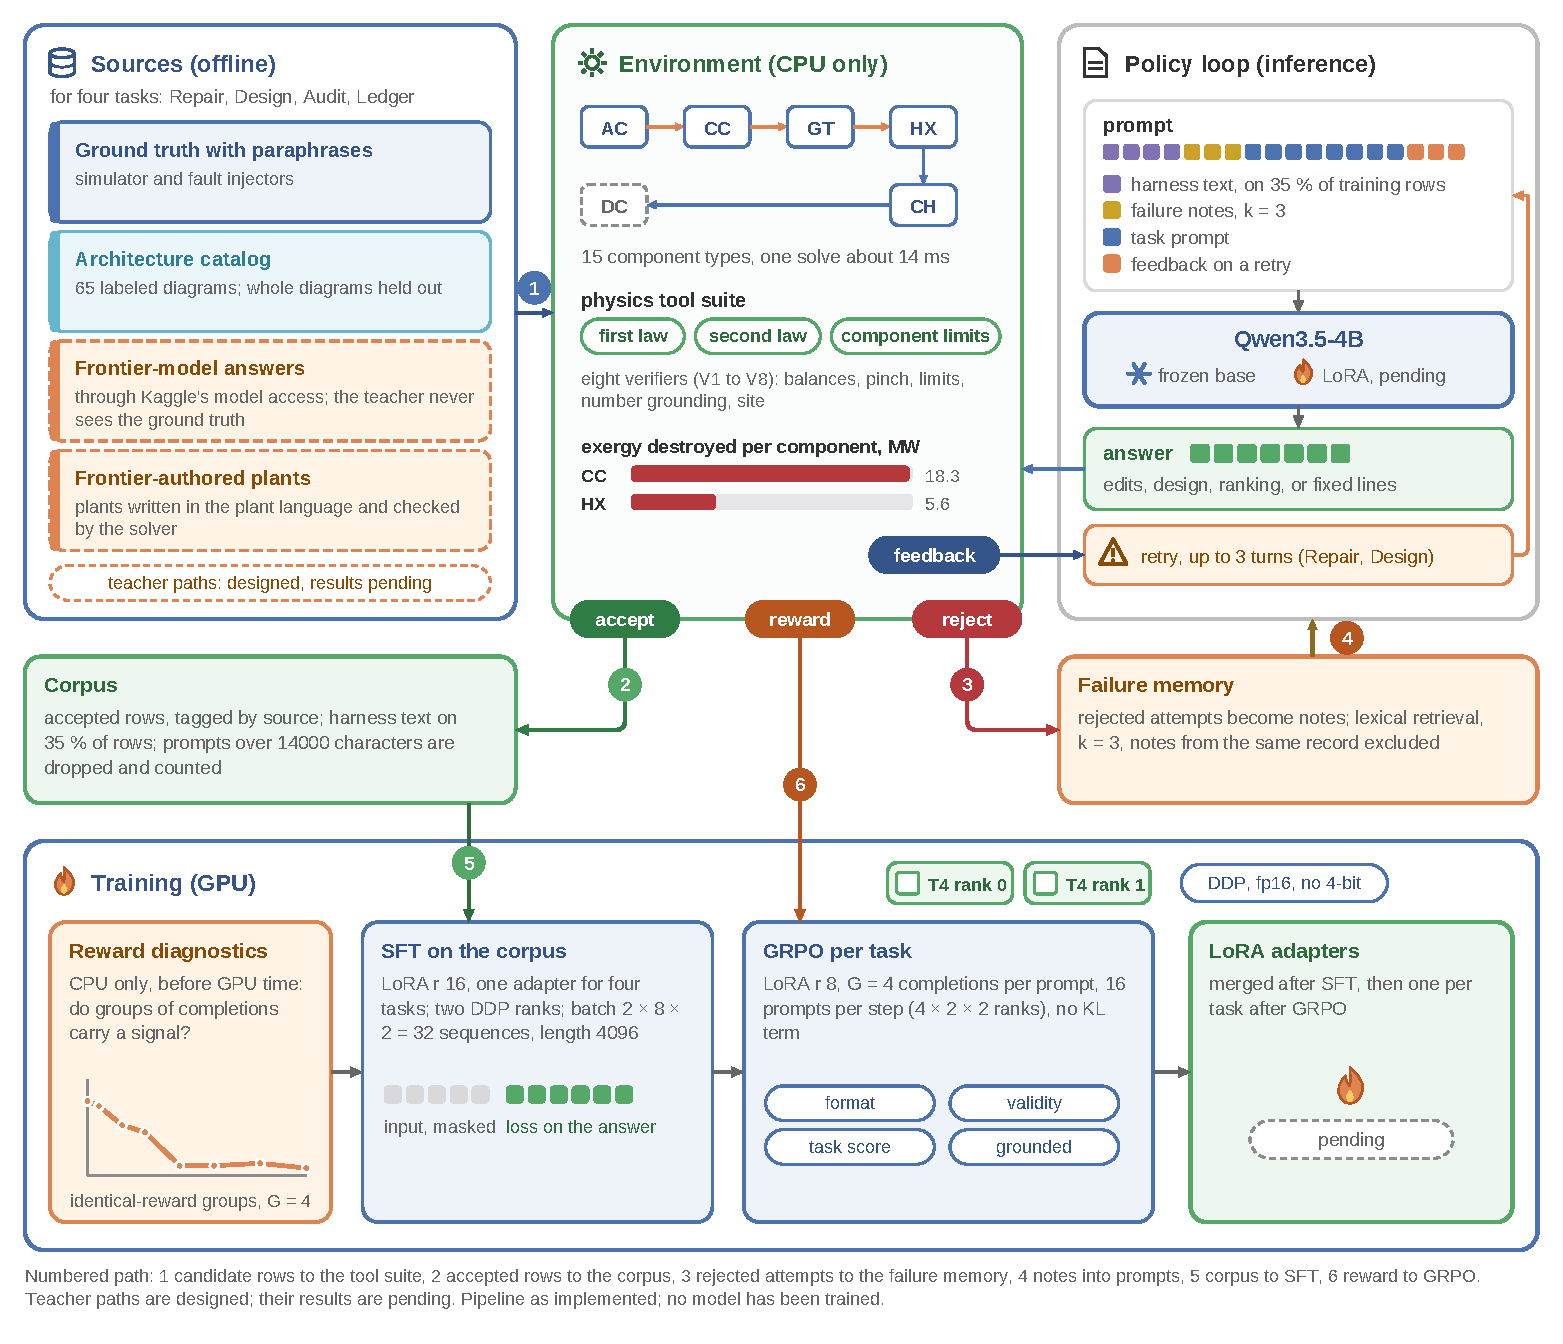
\includegraphics[width=\linewidth]{figures/pdf/fig_overview.pdf}
\caption{System overview. Offline, sampled plants, faults and a reference search give verified
expert answers for supervised fine-tuning and the reward for GRPO. The environment (simulator,
exergy accounting, verifiers V1 to V8) supplies the reward in training and the feedback at inference;
online, the model proposes an answer, the solver and the verifiers check it, and the model retries.
The figure shows the design, not results: no model has been trained, and every trained-model
statement is marked pending.}
\label{fig:fig_overview}
\end{figure}

\paragraph{Contributions.}
\begin{enumerate}[leftmargin=*,itemsep=2pt]
\item A second-law-verified environment for data-center energy systems: \val{env.n_components}
component models, exergy accounting against an explicit dead state, and verifiers V1 to V8
whose checks are the reward (\cref{sec:method}).
\item Four task families with structural out-of-distribution splits: Repair (parameter-level faults,
\val{env.n_repair_faults} types), Design (a catalog of \val{env.n_catalog} configurations,
\val{env.n_catalog_heat} when there is a heat demand, plus continuous parameters), Audit (rank
exergy destroyers, propose one allowed change, predict its fuel effect) and Ledger repair
(\val{env.n_ledger_faults} equation-level fault types in an exergy ledger, which range checks cannot
see).
\item An evaluation that counts solver calls: non-model baselines, an anytime protocol for sample
efficiency, paired statistics, and ablations that include an agent harness (an \texttt{AGENTS.md}
file plus generated skills) with a held-out component.
\item Simulator findings that do not depend on a model: feasibility limits of the catalog, first-law
against second-law blame, the symptom coverage of equation faults, and trace and modular-fleet bounds
(\cref{sec:experiments,sec:trace}).
\end{enumerate}

\paragraph{What we do not claim.}
We do not claim that a trained model beats numerical optimization on the final optimum for a fixed
superstructure. We do not claim any validation against a real plant, and there is no measured
on-site-generation data center in this work: measured load and coolant traces from published data
set the operating points of a physics model, and all training data is synthetic. No model has been
trained, so we make no claim about trained-model results; for the trained model we intend to claim
only sample efficiency and breadth, and only once the pending runs exist.

\paragraph{Paper map.}
\Cref{sec:related} places the work among related studies. \Cref{sec:method} describes the
environment, the verifiers, the tasks, the rewards, the training recipe and the agent harness.
\Cref{sec:experiments} states the frozen evaluation protocol, reports the non-model baselines and
simulator findings that were measured, and gives the skeletons of the pending model results.
\Cref{sec:trace} covers trace and fleet bounds, \cref{sec:limits} lists the limits, and the appendix
holds definitions, registries and the reproduction recipe.

\section{Related work}\label{sec:related}

\paragraph{Thermodynamics benchmarks and agents.}
ThermoQA is a benchmark of thermodynamic questions for language models; it is a single-author
preprint \citep{duzkar2026thermoqa}. Song et al.\ built ReAct agents for gas-path analysis of
gas turbines and found that smaller models struggled with tool use and parameter extraction
\citep{song2024gaspath}. Both evaluate models; neither trains one against a simulator.

\paragraph{Design and flowsheet agents.}
Text2Sim uses multiple prompted agents, with a frozen model, to turn a text description into a
chemical-process simulation \citep{tian2026text2sim}. Li et al.\ treat thermodynamic cycle co-design
as a graph-based hierarchical reinforcement-learning problem with a learned surrogate and no language
model \citep{li2026thermocycle}. Our Design task uses a language model to choose a configuration and
continuous parameters, but the final check is the physical simulator rather than a surrogate.

\paragraph{Reinforcement learning with verifiable and solver-grounded rewards.}
GRPO \citep{shao2024deepseekmath} and its use for reasoning \citep{guo2025deepseekr1} replace a learned
value function with group-normalized rewards. Tulu~3 introduced reinforcement learning with verifiable
rewards for post-training and motivates a supervised stage first: sparse verifiable rewards need a policy
that already succeeds sometimes \citep{lambert2024tulu3}. Solver-informed reinforcement learning uses
a solver in the loop for optimization modeling \citep{chen2025sirl}. Reinforcement learning from execution feedback
in code uses test outcomes as the reward \citep{gehring2024rlef}, and the loss we use follows the DAPO
variant of GRPO \citep{yu2025dapo}. The closest methodological precedent is Luo et al., who run
supervised fine-tuning followed by GRPO with a solver-grounded reward for modeling nuclear
thermal-hydraulic systems, with LoRA rank 8 and a group of 8; they report solver convergence rising
from 72.4\% after supervised fine-tuning to 88.8\% after GRPO \citep{luo2026nuclear}. Our work follows the same
two stages with a different reward: the physical second-law checks of \cref{sec:verifiers}.

\paragraph{Parameter-efficient reinforcement learning.}
LoRA \citep{hu2021lora} is the adapter method we use. Reinforcement learning has been reported to need little adapter capacity, with a learning
rate about ten times that of full fine-tuning \citep{schulman2025lora}; our GRPO stage uses a smaller
rank than the SFT stage for that reason. Adapting a decoder-only model into an encoder-decoder model
\citep{zhang2025t5gemma} is an optional ablation only, because reinforcement-learning tooling
targets decoder-only models.

\paragraph{Data-center on-site generation, waste heat and absorption cooling.}
Combined heat and power for data centers was assessed in an Oak Ridge report \citep{darrow2009chp}.
Published measurements of the Frontier supercomputer give the load and the coolant temperatures that
set our operating points \citep{sun2024frontier,jadhav2026frontierml}. The coefficient of performance
of a single-effect absorption chiller was measured at 0.55 to 0.70 with 88\,$^\circ$C hot water,
12.5\,$^\circ$C chilled water and 31\,$^\circ$C cooling water \citep{ochoa2019absorption}; our
absorption model is a system-level fraction of the reversible COP, capped at 0.8, not a property model
(\cref{sec:limits}). Exergy analysis and its use in design follows standard texts \citep{bejan1996thermal}.
Gas properties come from the GRI-Mech 3.0 polynomials \citep{smith1999grimech} and liquid properties
from CoolProp \citep{bell2014coolprop}.

\paragraph{Positioning.}
The ingredients exist: GRPO, verifiable rewards, solver-grounded reinforcement learning and language
models for process design. The combination for data-center energy systems, with second-law verifiers
as the reward, four task families with structural splits, an equation-level ledger benchmark and
accounting in solver calls, is what we contribute. \Cref{tab:positioning} summarizes how the cited
methods differ.

\begin{table}[tbp]
\centering\small\renewcommand{\arraystretch}{1.15}
\begin{tabular}{@{}p{3.4cm}p{1.9cm}p{2.4cm}p{2.4cm}p{1.7cm}p{1.7cm}@{}}
\toprule
Work & Language model & Trained with solver or verifier reward & Exergy or second-law checks & Data-center domain & Equation-level fault repair \\
\midrule
ThermoQA \citep{duzkar2026thermoqa} & evaluated & no & \todo{check} & no & no \\
Gas-path agents \citep{song2024gaspath} & prompted & no & \todo{check} & no & no \\
Text2Sim \citep{tian2026text2sim} & prompted, frozen & no & \todo{check} & no & no \\
Cycle co-design RL \citep{li2026thermocycle} & none (graph RL) & learned surrogate & \todo{check} & no & no \\
Solver-informed RL \citep{chen2025sirl} & trained & solver & \todo{check} & no & no \\
Nuclear TH modeling \citep{luo2026nuclear} & trained & solver & \todo{check} & no & no \\
\textbf{This work} (\sys) & to be trained & simulator and verifiers & yes (V3, V5) & yes & yes \\
\bottomrule
\end{tabular}
\caption{Positioning among cited work. Entries for prior work follow the descriptions recorded in
the project notes for each paper; ``no'' means the property is not part of the described method, and the
second-law column is not yet checked against the papers themselves. The last row describes the design;
the trained model is pending.}
\label{tab:positioning}
\end{table}

\section{Method}\label{sec:method}

The method has five parts: a plant simulator with exergy accounting (\cref{sec:env,sec:exergy}), verifiers
that decide whether a plant is acceptable (\cref{sec:verifiers}), four task families built on them
(\cref{sec:tasks,sec:rewards}), a verifier-gated training corpus with varied traces, a teacher model and a
retrievable success-and-failure memory (\cref{sec:corpus}), and a two-stage training recipe with an agent harness
(\cref{sec:training,sec:harness}). Constants marked as assumed are model settings, not measurements;
\cref{tab:constants} lists them and \cref{sec:limits} discusses what they do to the results.

\paragraph{Status at the time of writing.}
The simulator, verifiers, tasks, rewards and every simulator-driven number in this paper are measured and reproducible from checked-in generators and fixed seeds. The corpus-side datagen is complete: deterministic tool corpora at 4,800 rows per task family with equal-thirds tiers, the 1,600-row plain A-slice, the frozen \texttt{heldout\_v2} test set, the compact harness, the training-path fixes, per-row provenance and the token gate are all built and audited (\cref{sec:corpusstatus,sec:datagenstatus}). The frontier chain-of-thought campaign is \emph{in progress} with only two authorized budget models. The training and model-evaluation parts of the method (\cref{sec:corpus,sec:training,sec:harness}) remain a \emph{planned and pre-registered} recipe: no SFT step, GRPO step or model evaluation has run, and no checkpoint exists. Every training or decoding constant quoted below is a decided setting, not a measured result. Per Reza's directive of 2026-11-19, training starts only after all datagen items are built, audited and committed.

\subsection{The environment: plant graph, fluids and solver}\label{sec:env}

A plant is a typed graph. Components are nodes; streams are edges whose endpoints are either
\texttt{Comp.port} or \texttt{ext:name} for a boundary. Each port accepts one fluid class, gas or liquid, and a
mismatch is an error. Stream fluids are ideal-gas mixtures (\texttt{CGAM\_AIR}, \texttt{FLUE},
\texttt{CH4}), with NASA-7 polynomials from GRI-Mech~3.0 \citep{smith1999grimech} whose enthalpy includes
the formation enthalpy and whose entropy uses partial pressures, or CoolProp fluids \citep{bell2014coolprop}
(Water, R245fa, Cyclopentane, Toluene). A stream that has a component as its source and carries fixed
values is a tear stream: it closes a loop, and the producing component must reproduce it or the solver
reports non-convergence. The solver is sequential-modular with tear streams, on a molar basis in SI units. Errors are
typed (for example \texttt{E\_PROP\_RANGE}, \texttt{E\_TEMP\_CROSS}, \texttt{E\_NOT\_CONVERGED},
\texttt{E\_FLUID\_MISMATCH}, \texttt{E\_DISCONNECTED}, \texttt{E\_OVER\_SPECIFIED},
\texttt{E\_UNDER\_SPECIFIED}), so that a failed solve returns text a model can read. One solve of the plant in
\cref{fig:fig_exergy_flow} took \val{exf.solve_ms}\,ms on average over ten runs on the authoring machine (a single
CPU); the project's design notes give 10 to 30 ms.

\begin{figure}[tbp]
\centering
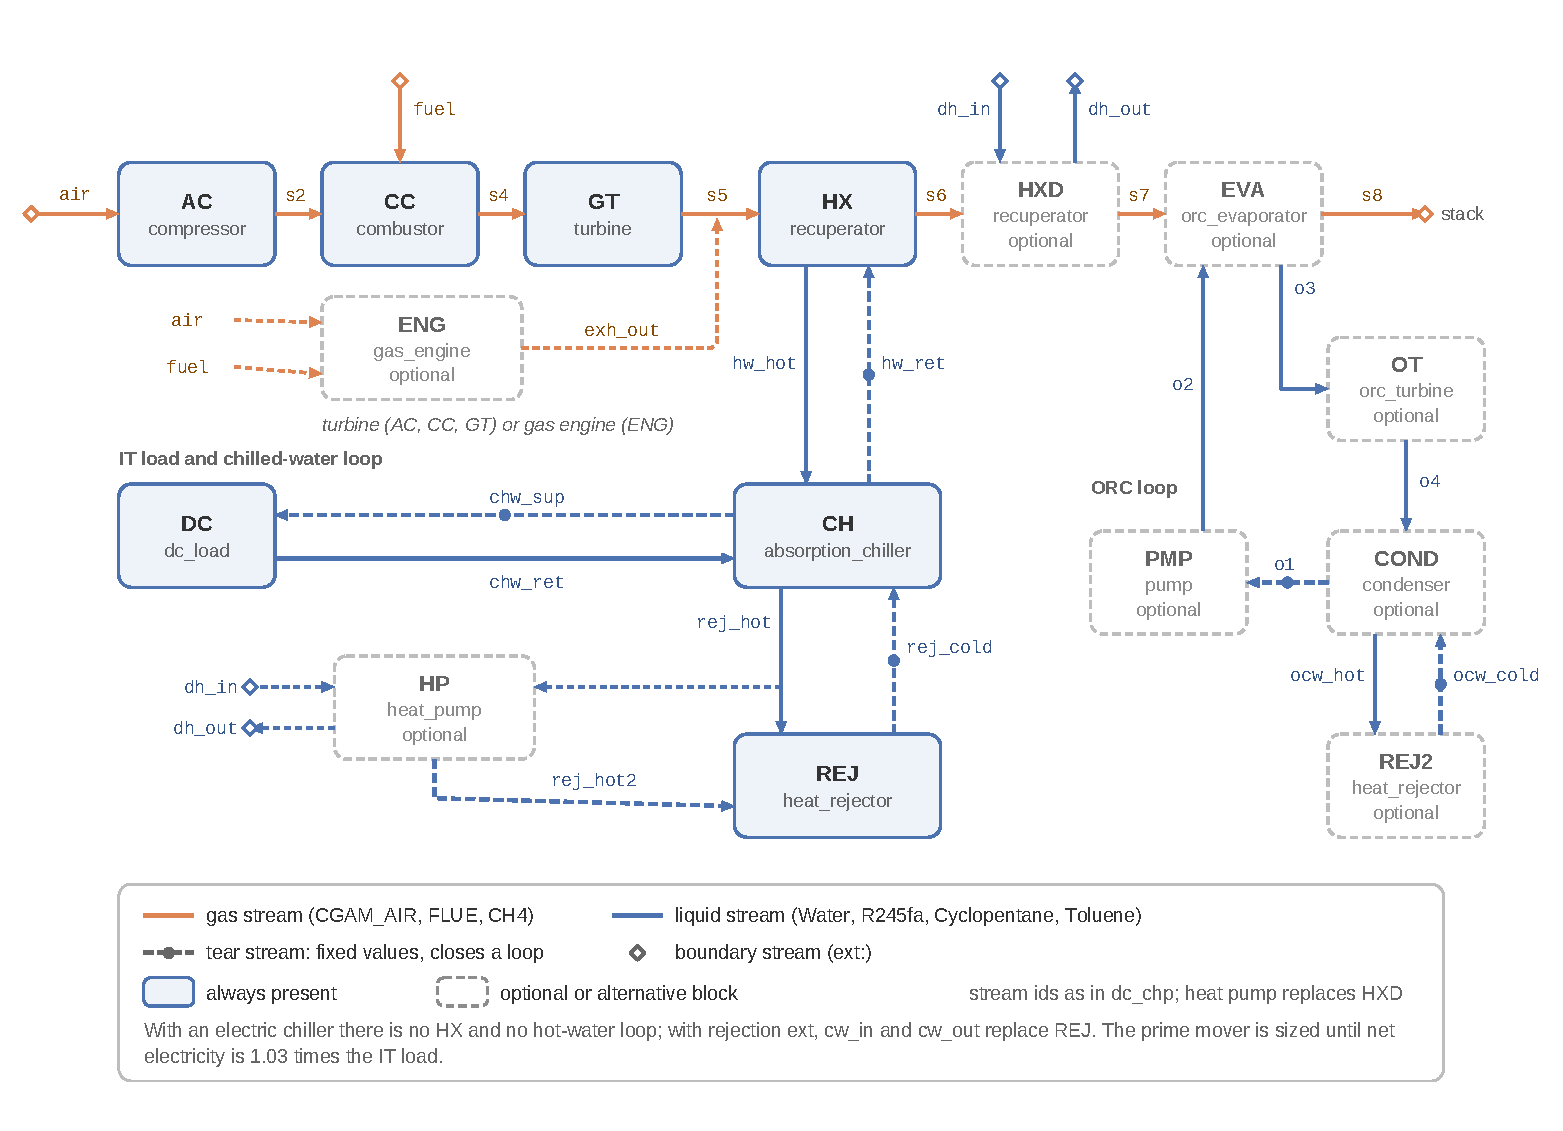
\includegraphics[width=\linewidth]{figures/pdf/fig_plant_graph.pdf}
\caption{Plant graph of the data-center model with the real stream identifiers. Gas streams are orange and liquid
streams blue; dashed streams are tear streams with fixed values that close a loop; dashed boxes are optional or
alternative blocks (gas engine, district-heat exchanger, ORC loop, second heat rejector, heat pump). The graph is
produced from three builder calls of the \texttt{dc\_chp} topology (\texttt{assets/plant\_graph.json}); it is a
structural diagram, not a result.}
\label{fig:fig_plant_graph}
\end{figure}

\paragraph{Component library.}
There are \val{env.n_components} component types with \val{env.n_params} registered parameters in total
(\cref{tab:components}; the full registry is in \cref{app:registry}). The main models are these. The combustor
solves a fuel-to-air mole ratio from an energy balance with a heat-loss fraction. The gas engine is sized by its
rated electrical output: fuel is $P_{\mathrm{el}}/(\eta_{\mathrm{el}}\,\mathrm{LHV})$, jacket and radiation heat
$f_{\mathrm{loss}}\,\dot n_F\,\mathrm{LHV}$ is rejected to ambient rather than recovered, and the exhaust
temperature follows from the balance. The absorption chiller has
$\mathrm{COP}=\min(\varepsilon\,\mathrm{COP}_{\mathrm{rev}},\mathrm{COP}_{\max})$ with $\varepsilon=0.27$ and a
cap of $0.8$, where $\mathrm{COP}_{\mathrm{rev}}$ is the reversible COP of the generator, rejection and
evaporator temperatures. Electric chillers and heat pumps use a fraction $\varepsilon=0.5$ of the reversible (Lorenz)
COP on refrigerant-side temperatures obtained by moving the stream log-mean temperatures outward by a 5~K approach.
The heat rejector's outlet is the dry-bulb temperature (dry cooler, 8~K approach) or the wet-bulb temperature (tower,
5~K approach) plus the approach; fans use 1.5\% of the heat rejected, and tower make-up water is an upper bound.
The ORC evaporator puts its pinch at the bubble point and lets the working-fluid flow lie in a window: the upper limit keeps the
exhaust above a stack floor of 333~K and the lower limit keeps the vapor at or below a fluid-specific temperature
(420, 480 and 560~K for R245fa, cyclopentane and toluene); if the lower limit exceeds the upper, the exhaust is too hot
for that fluid. The IT load consumes $P_{\mathrm{it}}$ of electricity and passes a fraction $f$ of it to a chilled-water
loop; the rest is rejected directly.

\begin{table}[tbp]
\centering
\begingroup\scriptsize\setlength{\tabcolsep}{4pt}\renewcommand{\arraystretch}{1.15}
\begin{tabular}{@{}p{3.2cm}p{4.9cm}p{7.0cm}@{}}
\toprule
Type & Ports (fluid class) & Parameters \\
\midrule
\texttt{compressor} & \texttt{in} (g), \texttt{out} (g) & \texttt{PR}, \texttt{eta\_s} \\
\texttt{turbine} & \texttt{in} (g), \texttt{out} (g) & \texttt{P\_out}, \texttt{eta\_s} \\
\texttt{orc\_turbine} & \texttt{in} (l), \texttt{out} (l) & \texttt{P\_out}, \texttt{eta\_s} \\
\texttt{pump} & \texttt{in} (l), \texttt{out} (l) & \texttt{P\_out}, \texttt{eta\_s} \\
\texttt{combustor} & \texttt{air\_in} (g), \texttt{fuel\_in} (g), \texttt{out} (g) & \texttt{T\_out}, \texttt{dp}, \texttt{q\_loss} \\
\texttt{recuperator} & \texttt{cold\_in} (?), \texttt{cold\_out} (?), \texttt{hot\_in} (?), \texttt{hot\_out} (?) & \texttt{T\_cold\_out}, \texttt{dp\_cold}, \texttt{dp\_hot}, \texttt{useful\_heat} \\
\texttt{hrsg} & \texttt{hot\_in} (g), \texttt{hot\_out} (g), \texttt{water\_in} (l), \texttt{steam\_out} (l) & \texttt{P\_steam}, \texttt{dp\_gas}, \texttt{econ\_approach\_K} \\
\texttt{orc\_evaporator} & \texttt{hot\_in} (g), \texttt{hot\_out} (g), \texttt{cold\_in} (l), \texttt{cold\_out} (l) & \texttt{pinch\_K}, \texttt{dp\_hot}, \texttt{flow\_frac}, \texttt{T\_stack\_min}, \texttt{T\_max\_K} \\
\texttt{condenser} & \texttt{hot\_in} (l), \texttt{hot\_out} (l), \texttt{cold\_in} (l), \texttt{cold\_out} (l) & \texttt{dT\_cw} \\
\texttt{dc\_load} & \texttt{in} (l), \texttt{out} (l) & \texttt{P\_it}, \texttt{chilled\_fraction}, \texttt{T\_return} \\
\texttt{absorption\_chiller} & \texttt{gen\_in} (l), \texttt{gen\_out} (l), \texttt{evap\_in} (l), \texttt{evap\_out} (l), \texttt{rej\_in} (l), \texttt{rej\_out} (l) & \texttt{T\_chw\_out}, \texttt{T\_gen\_out}, \texttt{dT\_rej}, \texttt{eps}, \texttt{COP\_max} \\
\texttt{heat\_pump} & \texttt{src\_in} (l), \texttt{src\_out} (l), \texttt{sink\_in} (l), \texttt{sink\_out} (l) & \texttt{T\_sink\_out}, \texttt{eps}, \texttt{approach\_K}, \texttt{Q\_sink}, \texttt{dT\_src} \\
\texttt{electric\_chiller} & \texttt{evap\_in} (l), \texttt{evap\_out} (l), \texttt{rej\_in} (l), \texttt{rej\_out} (l) & \texttt{T\_chw\_out}, \texttt{dT\_rej}, \texttt{eps}, \texttt{approach\_K} \\
\texttt{heat\_rejector} & \texttt{in} (l), \texttt{out} (l) & \texttt{kind}, \texttt{approach\_K}, \texttt{fan\_frac} \\
\texttt{gas\_engine} & \texttt{air\_in} (g), \texttt{fuel\_in} (g), \texttt{exh\_out} (g) & \texttt{P\_el}, \texttt{eta\_el}, \texttt{f\_loss}, \texttt{air\_excess}, \texttt{P\_exh} \\
\bottomrule
\end{tabular}\endgroup

\caption{Component library, generated from \texttt{core.components} (\texttt{REQUIRED\_PORTS},
\texttt{PORT\_CLASS}, \texttt{PARAMS}). Ports are marked g (gas) or l (liquid).}
\label{tab:components}
\end{table}

\paragraph{Sizing and topologies.}
The prime mover (the air flow of a turbine or the rated power of an engine) is scaled by secant iteration on full
plant solves until net electricity (generation minus parasitics plus ORC output) equals $1.03\,P_{\mathrm{it}}$. Two
topology families are used. The first is a gas turbine with an air preheater, an HRSG and an R245fa ORC, which is held
out as the steam-ORC topology. The second is the data-center plant \texttt{dc\_chp}: a prime mover (turbine or engine), cooling
(absorption or electric), heat rejection (an ideal boundary, a dry cooler or a wet tower), optional ORC bottoming with
one of three fluids, and optional district heat from the exhaust (a heat exchanger) or from a heat pump on the chiller
rejection water.

\paragraph{Cross-check.}
The generic engine was checked against an independent reference implementation of a gas turbine with an HRSG and an
R245fa ORC (one operating point, $n=1$). Net power agrees to \val{xchk.wnet_rel_pct}\%, energy efficiency to
\val{xchk.etaI_rel_pct}\%, and the HRSG pinch to \val{xchk.pinch_diff_K}~K; exergy closure holds to
\val{xchk.closure_w}~W, and component destruction agrees to \val{xchk.ed_max_rel_pct}\% or better. Exergy efficiency is
\val{xchk.etaII_diff_pct}\% (engine relative to reference), because chemical exergy is computed from the Gibbs energy of
the fuel reaction. This is a consistency check of the implementation, not a validation against a real plant.

\begin{table}[tbp]
\centering
\begingroup\small\renewcommand{\arraystretch}{1.12}
\begin{tabular}{@{}p{7.2cm}p{4.6cm}p{3.6cm}@{}}
\toprule
Constant (assumed, not fitted) & Code name & Default \\
\midrule
Compressor isentropic efficiency & \texttt{eta\_c} & 0.86 \\
Turbine isentropic efficiency & \texttt{eta\_t} & 0.88 \\
Pressure ratio & \texttt{PR} & 18 \\
Turbine inlet temperature (K) & \texttt{T4} & 1500 \\
Combustor pressure drop; heat loss fraction & \texttt{dp\_cc}, \texttt{q\_loss} & 0.04; 0.01 \\
Gas engine electrical efficiency & \texttt{eta\_el} & 0.43 \\
Gas engine loss fraction (jacket and radiation) & \texttt{f\_loss} & 0.15 \\
Air excess & \texttt{air\_excess} & 1.8 \\
Absorption chiller: fraction of reversible COP; COP cap & \texttt{eps\_abs}, \texttt{COP\_max} & 0.27; 0.8 \\
Electric chiller and heat pump: fraction of reversible COP & \texttt{eps\_ec}, \texttt{eps\_hp} & 0.5; 0.5 \\
Chilled-water supply and return (K) & \texttt{T\_supply}, \texttt{T\_return} & 291.15; 301.15 \\
Hot-water loop supply and return (K) & \texttt{T\_hw}, \texttt{T\_gen\_out} & 368.15; 358.15 \\
Rejector approach to ambient (dry or wet; K) & \texttt{dT\_rej} & 8 (dry), 5 (wet) \\
Rejector fan power (share of heat rejected) & \texttt{fan\_frac} & 0.015 \\
ORC working-fluid vapour limits (K) & \texttt{ORC\_T\_MAX} & R245fa 420; Cyclopentane 480; Toluene 560 \\
ORC condenser approach (K); pump and turbine efficiency & \texttt{orc\_cond\_approach}, \texttt{eta\_pump}, \texttt{eta\_orct} & 8; 0.75; 0.85 \\
Stack temperature floor for exhaust recovery (K) & \texttt{T\_stack\_min} & 333.15 \\
Fraction of the IT heat on the chilled-water loop & \texttt{chilled\_fraction} & 0.5 (Design: site input) \\
Sizing margin on net electricity & \texttt{margin} & 1.03 \\
\bottomrule
\end{tabular}\endgroup

\caption{Assumed technology constants with their code defaults (\texttt{synth/topologies.py}, \texttt{core.components}). They are model settings, not measurements.}
\label{tab:constants}
\end{table}

\subsection{Exergy accounting}\label{sec:exergy}

The dead state is $(T_0,P_0)$ with the ambient air composition. For a stream at $(T,P)$ the physical exergy per mole is
\begin{equation}
e_{\mathrm{ph}}=(h-h_0)-T_0\,(s-s_0),
\end{equation}
with $h_0,s_0$ evaluated at $(T_0,P_0)$ for the same composition. The chemical exergy of a gas mixture is
\begin{equation}
e_{\mathrm{ch}}=\sum_i y_i\,\varepsilon_i+R\,T_0\sum_i y_i\ln y_i,
\end{equation}
where $\varepsilon_i=-R\,T_0\ln y_{\mathrm{env},i}$ for the species present in the environment, so that ambient air has exactly
zero exergy, and $\varepsilon_{\mathrm{CH_4}}=-\Delta G+\varepsilon_{\mathrm{CO_2}}+2\varepsilon_{\mathrm{H_2O}}-2\varepsilon_{\mathrm{O_2}}$
with $\Delta G$ the Gibbs energy change of $\mathrm{CH_4}+2\,\mathrm{O_2}\rightarrow\mathrm{CO_2}+2\,\mathrm{H_2O(g)}$ at $(T_0,1~\mathrm{atm})$.
Liquids carry no chemical exergy. The exergy destruction of a component is
\begin{equation}
\ED=\sum_{\mathrm{in}}\dot n\,e-\sum_{\mathrm{out}}\dot n\,e-\dot W_{\mathrm{out}},
\end{equation}
and heat dissipated to the ambient carries no exergy. Over the plant,
$\sum\ED=\sum_{\text{ext. in}}\dot n\,e-\sum_{\text{ext. out}}\dot n\,e-\sum\dot W$ (closure), which holds to machine precision in the tests. The
exergy efficiency is
\begin{equation}
\eta_{\mathrm{II}}=\frac{\dot W_{\mathrm{net}}+\Delta\dot E_{\text{steam, heat, chilled water}}}{\dot E_{\mathrm{fuel}}}.
\end{equation}
\Cref{fig:fig_exergy_flow} shows one solved plant: a gas turbine with absorption cooling, a dry cooler and
district heat from the exhaust at a 20~MW IT load. Of \val{exf.fuel_mw}~MW of fuel exergy, \val{exf.cc_mw}~MW
(\val{exf.cc_share_pct}\%) is destroyed in the combustor, \val{exf.stack_mw}~MW leaves with the stack, and the delivered
cooling and heat carry only \val{exf.cool_ex_mw} and \val{exf.heat_ex_mw}~MW of exergy although they are
\val{exf.cool_mw} and \val{exf.heat_mw}~MW of energy. The heat rejector dissipates \val{exf.rej_energy_mw}~MW of energy
but destroys only \val{exf.rej_ed_mw}~MW of exergy, which is the contrast that \cref{sec:findings} measures over many plants.

\begin{figure}[tbp]
\centering
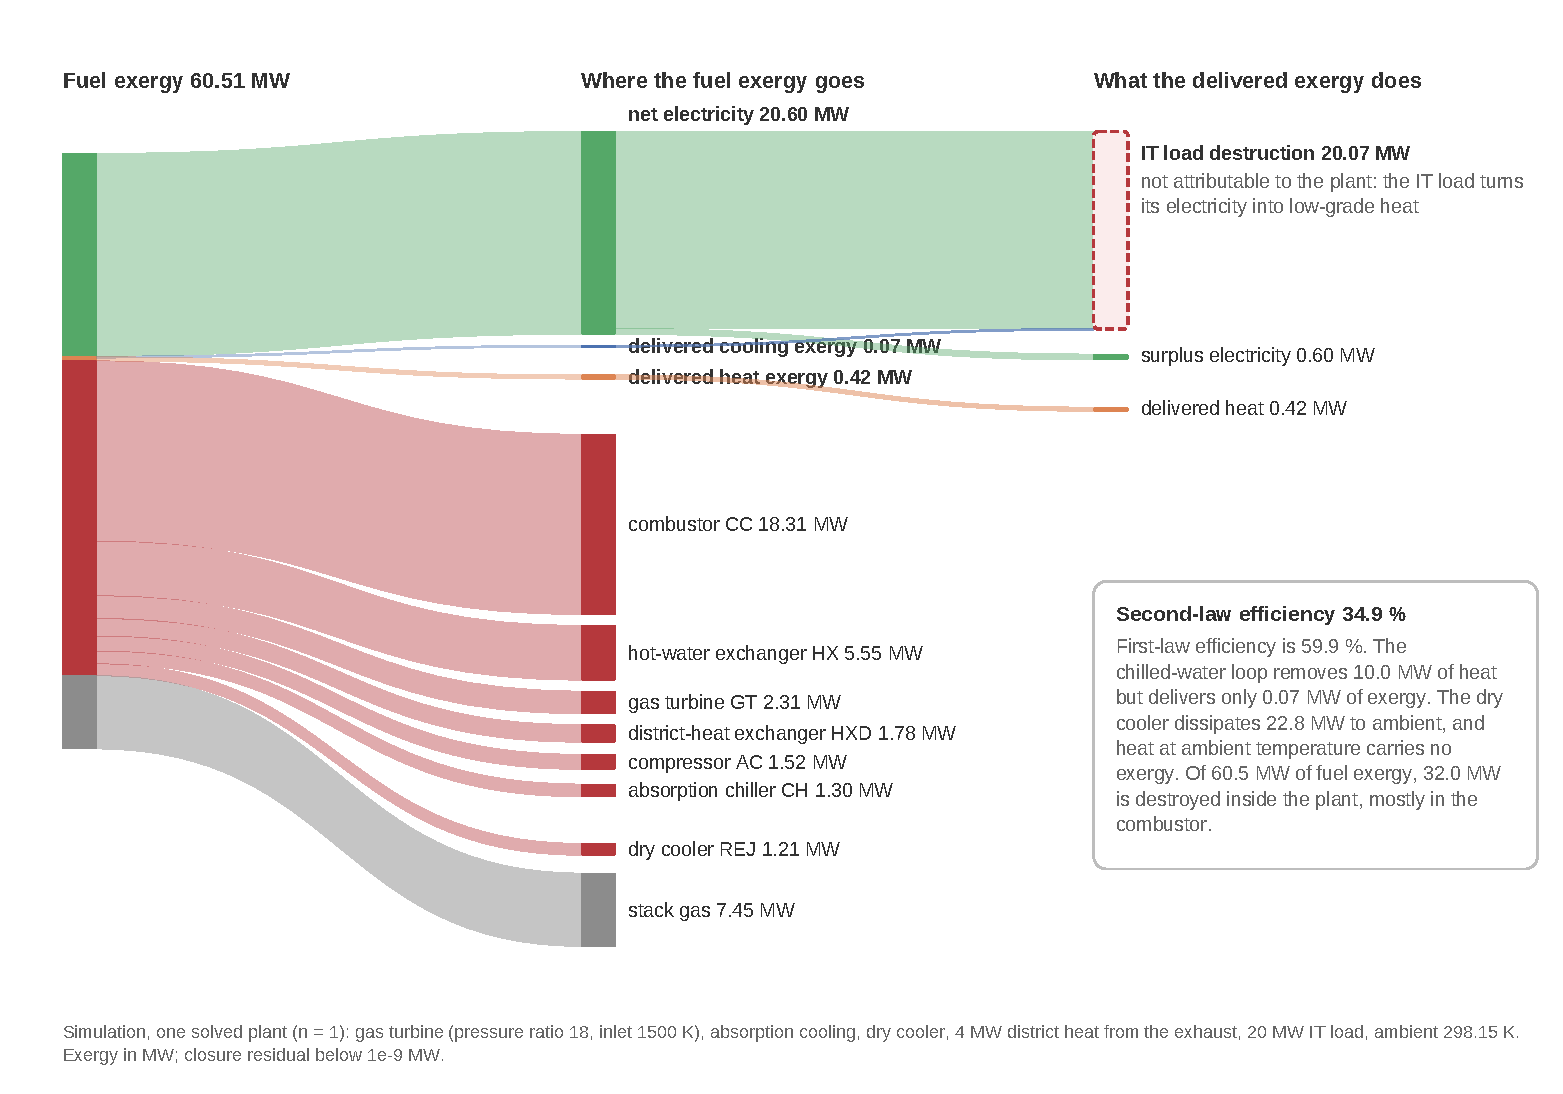
\includegraphics[width=\linewidth]{figures/pdf/fig_exergy_flow.pdf}
\caption{Exergy flow of one solved plant ($n=1$, simulation): gas turbine, absorption cooling, dry cooler, district heat
from the exhaust, 20~MW IT load. Ribbon widths are proportional to MW of exergy. Most fuel exergy is destroyed in the
combustor; cooling and heat are small in exergy terms; the destruction in the IT load itself
(\val{exf.dc_mw}~MW) is not attributable to the plant. Data: \texttt{assets/exergy\_flow.json}.}
\label{fig:fig_exergy_flow}
\end{figure}

\subsection{Verifiers}\label{sec:verifiers}

Eight verifiers decide whether a plant is acceptable (\cref{tab:verifiers}); the same checks are the reward
(\cref{sec:rewards}) and the feedback at inference. Hard checks gate validity; soft checks only lower a score.
V1 and V2 are balance checks. V3a requires non-negative destruction in every component, and V3b requires the closure
of \cref{sec:exergy}; together they are the second-law checks on the model itself. V4a rejects a temperature cross in any heat
exchanger, and V4b asks for a practical pinch of 1~K. V5 bounds the efficiencies and every COP by the reversible limit of its stream temperatures.
V6 holds parameter and state ranges and is what catches most parameter-level faults. V7 grounds the numbers in a model's reasoning text, and V8
checks that the plant serves the site.

\begin{table}[tbp]
\centering
\begingroup\small\renewcommand{\arraystretch}{1.15}
\begin{tabular}{@{}lp{3.3cm}p{7.6cm}p{1.9cm}@{}}
\toprule
ID & Check & Definition and tolerance & Kind \\
\midrule
V1 & mass balance & per component, residual $\le 10^{-6}$ of the largest flow & hard \\
V2 & energy balance & per component, residual $\le 10^{-6}\,(|\dot W_{\text{net}}|+\dot Q_{\text{fuel}}+1~\mathrm{MW})$ & hard \\
V3a & non-negative destruction & $\ED \ge -10^{-5}\,\dot E_{\text{fuel}}$ in every component & hard \\
V3b & exergy closure & $|\sum \ED - (\text{in} - \text{out} - \dot W_{\text{net}})| \le 10^{-6}\,\dot E_{\text{fuel}}$ & hard \\
V4a & temperature cross & minimum approach $\ge 0$ K in every heat exchanger & hard \\
V4b & practical pinch & minimum approach $\ge 1$ K & soft \\
V5 & second-law bounds & $0\le\eta_{\mathrm{II}}\le 1$; power efficiency $<1-\Tzero/T_{\max}$; ORC efficiency $<1-T_{\mathrm{cond}}/T_{\mathrm{hot}}$; every COP at or below its reversible limit & hard \\
V6 & parameter and state ranges & efficiencies in $(0,1]$, pressure ratio $>1$, drops in $[0,0.3]$, $T$ in 150--2500 K, $P$ in 1 kPa--100 MPa, pressure-change direction & hard \\
V7 & number grounding & numbers with units in reasoning text match solver or plant values within 0.5\% (3\% for predicted Design quantities) & reward channel \\
V8 & site requirements & IT load within 1\%, electricity balance (no grid import unless allowed), cooling and heat $\ge 99\%$, water limit & hard (site) \\
\bottomrule
\end{tabular}\endgroup

\caption{Verifiers V1 to V8 with tolerances. Hard checks gate validity.}
\label{tab:verifiers}
\end{table}

\begin{figure}[tbp]
\centering
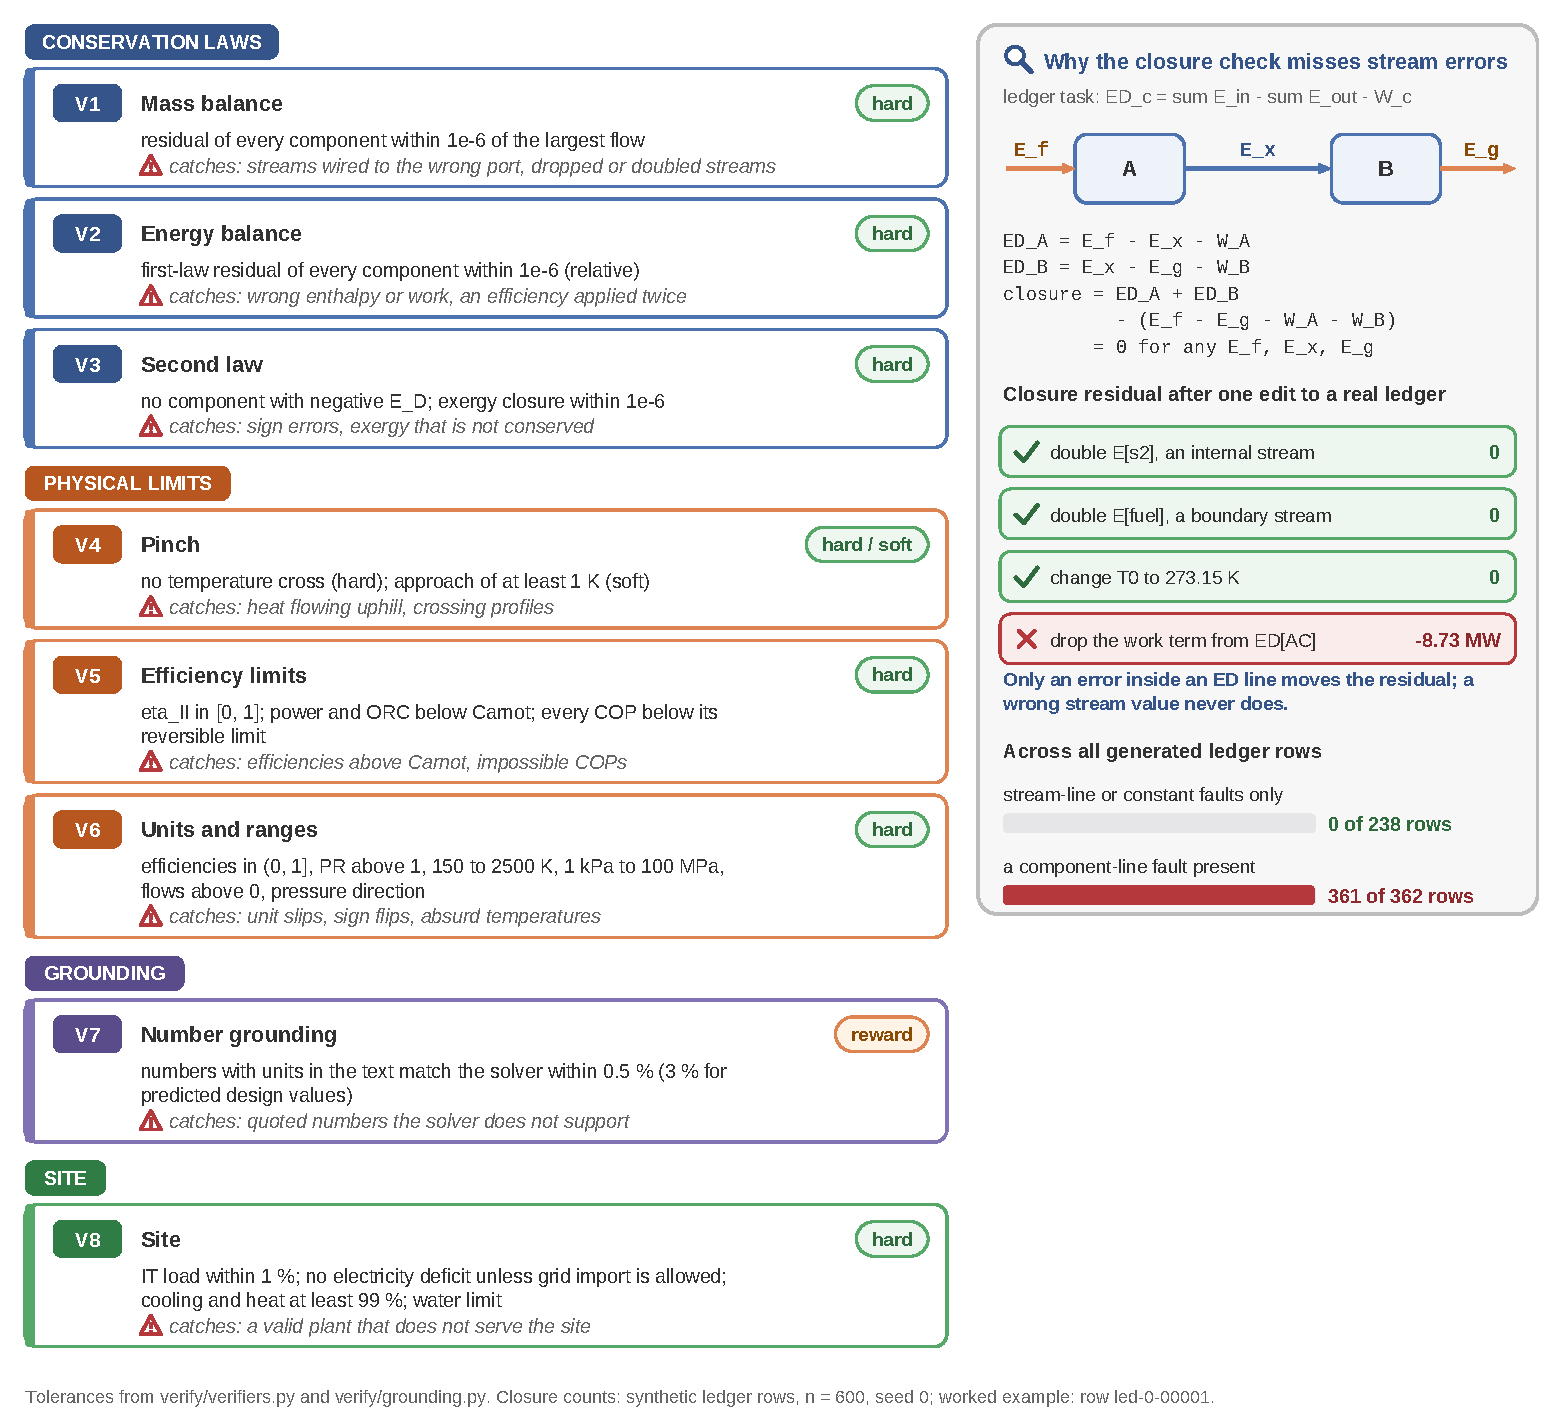
\includegraphics[width=\linewidth]{figures/pdf/fig_verifiers.pdf}
\caption{Verifiers V1 to V8 with tolerances and what each catches (left). Right: in the ledger task an error in any
stream value or in $T_0$ enters the closure sum with opposite signs and cancels; only errors in the destruction lines break
closure. The counts are from \val{led.n} generated ledger rows (seed 0, simulation): closure is broken in
\val{led.comp_closure} of \val{led.comp_rows} rows with a component-line fault and in \val{led.stream_closure} of
\val{led.stream_rows} rows with only stream-line or constant faults. Data: \texttt{assets/ledger\_symptoms.json}.}
\label{fig:fig_verifiers}
\end{figure}

\subsection{Tasks}\label{sec:tasks}

All four tasks are text in and text out. Plants are shown in a compact text language with one line per component
(\texttt{C id type \{params\}}) and per stream (\texttt{S id from -> to fluid \{extras\}}). \Cref{tab:tasks} summarizes the
tasks and \cref{fig:fig_tasks} shows verbatim excerpts of generated rows. The fault catalogs are in
\cref{app:faults}. Splits are structural: whole fault types, topologies or operating regimes are held out, and the rest
is split by a hash of the example identifier.

\begin{table}[tbp]
\centering
\begingroup\scriptsize\renewcommand{\arraystretch}{1.2}
\begin{tabular}{@{}p{1.5cm}p{3.2cm}p{2.8cm}p{3.3cm}p{3.3cm}@{}}
\toprule
Task & Input & Output & Reward channels (weight) & Held-out splits \\
\midrule
Repair & plant text, site, solver error or failed checks & \texttt{<diagnosis>}, at most 6 edits & format~0.5, valid~2, site~1, exact~1, minimal~0.5, grounded~0.5 & test ood fault: sign flip, swapped ports; test ood topology: 9 of 65 diagrams: the steam plant and the 8 gas-engine plants with ideal rejection \\
Design & site: IT load, chilled load, ambient $T$ and RH, coolant temperatures, optional heat demand and water limit & \texttt{<rationale>}, \texttt{<design>} block & format~0.5, valid~2, quality~2, grounded~0.5 & test ood scale: IT load of 45 MW or more; test ood climate: ambient 305 K or more; test ood load: chilled fraction 0.85 or more \\
Audit & solved plant with an energy-level summary & \texttt{<analysis>}, \texttt{<ranking>}, one \texttt{<change>}, \texttt{<prediction>} & format~0.5, rank~1.5, valid~1, gain~2, pred~1, grounded~0.5 & test ood topology: 9 of 65 diagrams: the steam plant and the 8 gas-engine plants with ideal rejection \\
Ledger repair & exergy ledger of a solved plant (arithmetic lines) & \texttt{<diagnosis>}, \texttt{FIX} lines & format~0.5, closure~1, nonneg~0.5, exact~2.5, minimal~0.5, grounded~0.5 & test ood fault: dropped\_work, wrong\_ref, wrong\_stream; test ood topology: 9 of 65 diagrams: the steam plant and the 8 gas-engine plants with ideal rejection \\
\bottomrule
\end{tabular}\endgroup

\caption{The four tasks: input, output, reward channels with weights (\cref{sec:rewards}) and held-out splits. Split
sizes are in \cref{app:datasets}.}
\label{tab:tasks}
\end{table}

\paragraph{Repair.}
A valid plant is broken by one of \val{env.n_repair_faults} fault types (unit slip, sign flip, efficiency above 1,
swapped ports, wrong fluid). The model reads the plant, the site and the solver or verifier output, and answers with
a diagnosis and at most six edits (\texttt{SET comp.param = x}, \texttt{SET @stream.field = x},
\texttt{REWIRE @stream.to = comp.port}, \texttt{FLUID @stream = fluid}) on existing numbers, endpoints and fluids. Every
injected fault that is kept is detected by the solver or the verifiers once the site specification is attached; most are
caught by range checks, which is why the Ledger task exists. The held-out splits are sign flip and swapped ports
(\texttt{test\_ood\_fault}) and the steam-ORC and gas-engine plants (\texttt{test\_ood\_topology}).

\paragraph{Design.}
The input is a site: IT load, chilled load, ambient temperature and humidity, coolant temperatures, and optionally a heat
demand and a water limit. The output is a \texttt{<rationale>} and a \texttt{<design>} block. The catalog combines prime mover
(turbine, engine), cooling (absorption, electric), rejection (dry, wet) and bottoming (none or an ORC on R245fa, cyclopentane
or toluene), which gives \val{env.n_catalog} configurations, doubled to \val{env.n_catalog_heat} by the heat source (exhaust or heat pump)
when there is a heat demand; seven continuous parameters (\texttt{dT\_rej}, \texttt{PR}, \texttt{T4}, \texttt{T\_hw}, \texttt{dT\_hw},
\texttt{P\_orc\_bar}, \texttt{orc\_frac}) complete a design. The objective is the least fuel among valid plants, with the services fixed by
the site. The reference is enumeration of the defaults followed by a Nelder--Mead polish of the best two; it is the best design found by this search, not a proven
optimum. Held-out regimes are an IT load of 45~MW or more, an ambient temperature of 305~K or more, and a chilled fraction of 0.85 or more.

\paragraph{Audit.}
The input is a solved plant with an energy-level summary; exergy destruction is hidden. The output is a ranking of exergy
destroyers, one allowed change (a set-point or loss parameter within $[0.8,1.25]$ of its value; component efficiencies and tear-closing temperatures
are excluded on purpose) and a prediction of the fuel change in MW after the prime mover is re-sized to the same net electricity.
The combustor or engine was the largest destroyer in every plant generated, so the ranking is scored with it removed.

\paragraph{Ledger repair.}
The exergy ledger of a solved plant is a list of arithmetic lines: \texttt{T0 = ...}; for every stream
\texttt{E[x] = m[x]*(h[x] - T0*s[x] - g0[x] + ech[x])/1e6}; for every component
\texttt{ED[c] = sum E[in] - sum E[out] - W[c]}. \val{env.n_ledger_faults} equation-level fault types in three layers
(stream lines, component lines, the constant) are injected into one or two lines; the model sees the ledger, the topology, the ambient
temperature, the stream values and the evaluated result, and answers with up to four corrected lines. Lines are evaluated by a
restricted arithmetic evaluator and nothing is executed. The held-out fault types are \texttt{wrong\_stream}, \texttt{dropped\_work} and
\texttt{wrong\_ref}. A program that rebuilds every line from the topology solves every row by construction, so the task measures whether a
model applies that rule from text and localizes the fault; this is a property of the benchmark, not an achievement of a model.

\begin{figure}[tbp]
\centering
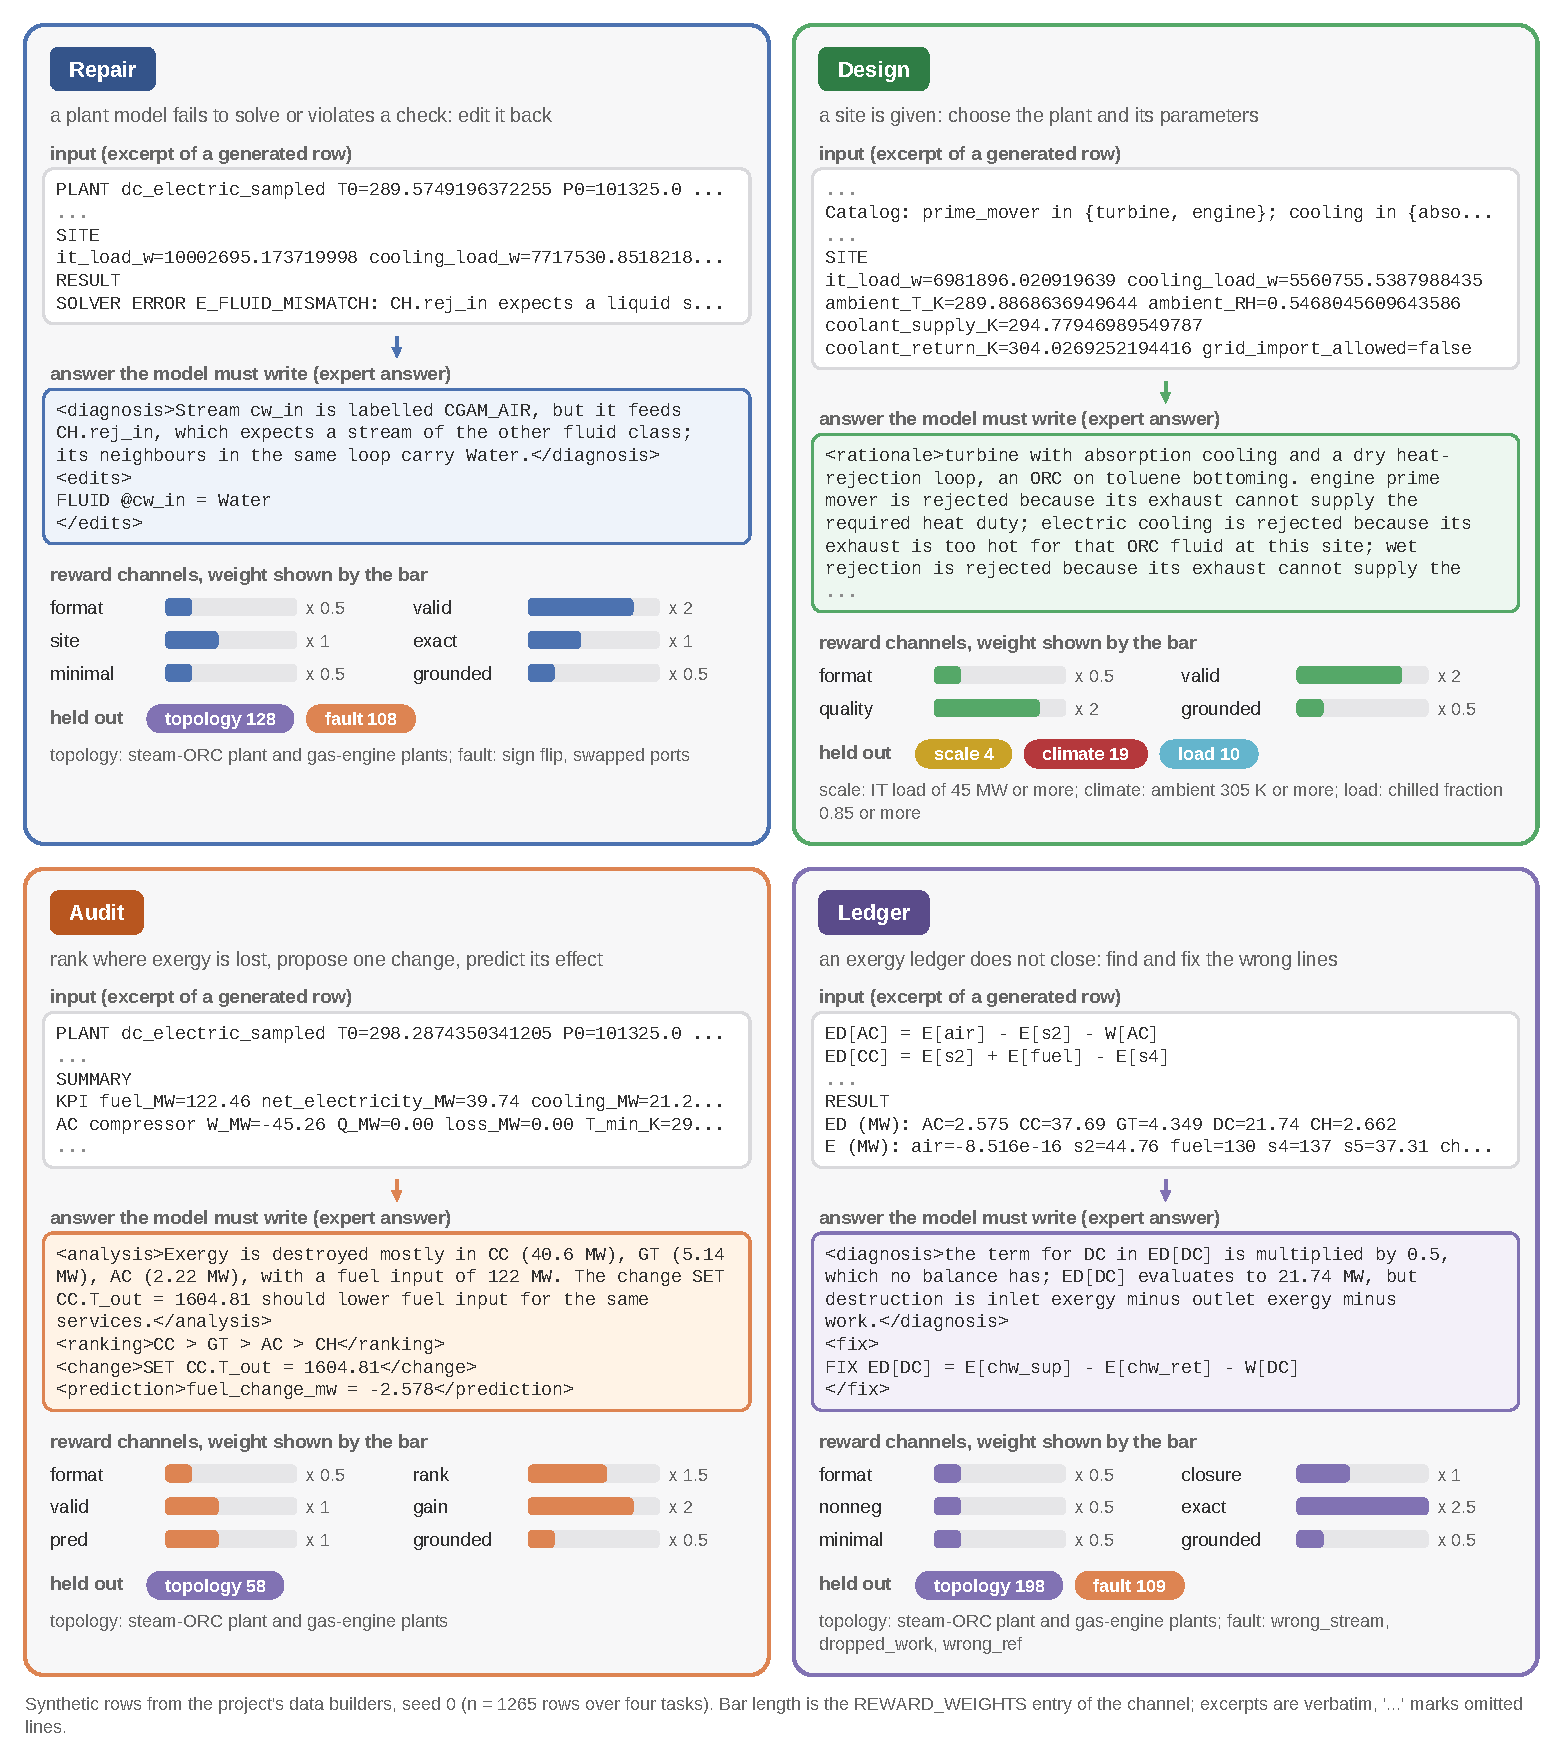
\includegraphics[width=\linewidth]{figures/pdf/fig_tasks.pdf}
\caption{The four tasks. For each: an excerpt of a generated input row, the expert answer the model must write, the reward
channels with their weights, and the held-out splits with row counts. Excerpts are verbatim from one generated training row
per task (seed 0; the row at the 12.5th length percentile); `\ldots' marks omitted lines. Data:
\texttt{assets/excerpts.json}, \texttt{assets/splits.json} (simulation, synthetic rows).}
\label{fig:fig_tasks}
\end{figure}

\subsection{Rewards}\label{sec:rewards}

Each task has its own channels; all are computed by the simulator and the verifiers, with no learned judge. Weights are in
\cref{tab:tasks}. \emph{Format} (0.5) rewards a parseable answer. \emph{Validity} (2 in Repair and Design, 1 in Audit) gives 1 if the plant
solves and passes every hard check and a partial credit otherwise (Repair: 0.5 times the fraction of checks passed; Design: 0.2 for a built but invalid plant).
\emph{Site} (1, Repair) requires the repaired plant to serve the site, so that deleting load is not a repair. \emph{Exact restoration} (1, Repair) applies only when the
original value is deducible from the broken plant. \emph{Minimality} rewards $1/(1+\text{extra edits})$. \emph{Quality} (2, Design) is
$1-(F-F_{\mathrm{ref}})/(0.1\,F_{\mathrm{ref}})$ clipped to $[0,1.05]$, so it is 1 at the reference fuel and 0 at 10\% more. In Audit, \emph{rank} (1.5) is nDCG@3 with the prime mover
removed, \emph{gain} (2) is the saved fuel divided by the best allowed saving, and \emph{prediction} (1) is
$1-|\hat y-y|/\max(|y|,0.002\,F)$. In Ledger repair, \emph{closure} (1) is 1 when the residual is within $10^{-6}$ of fuel exergy and falls to 0 at 1\%, \emph{non-negativity} (0.5) is the
share of components with $\ED\ge0$, and \emph{exactness} (2.5) counts faulty lines that now evaluate to the true value minus correct lines that are now broken. \emph{Grounding} (0.5) uses V7: every
number with a unit in the reasoning must match a solver or plant value.

Reward hacking is limited in three ways. Edits are restricted to existing fields, endpoints and fluids, so a model cannot add a component. The site check is part of the
Repair reward. The project's tests fuzz each reward function with junk and mutated answers and require that it never raises and stays bounded; this does not prove that
gaming is impossible, and we do not claim it.

\begin{figure}[tbp]
\centering
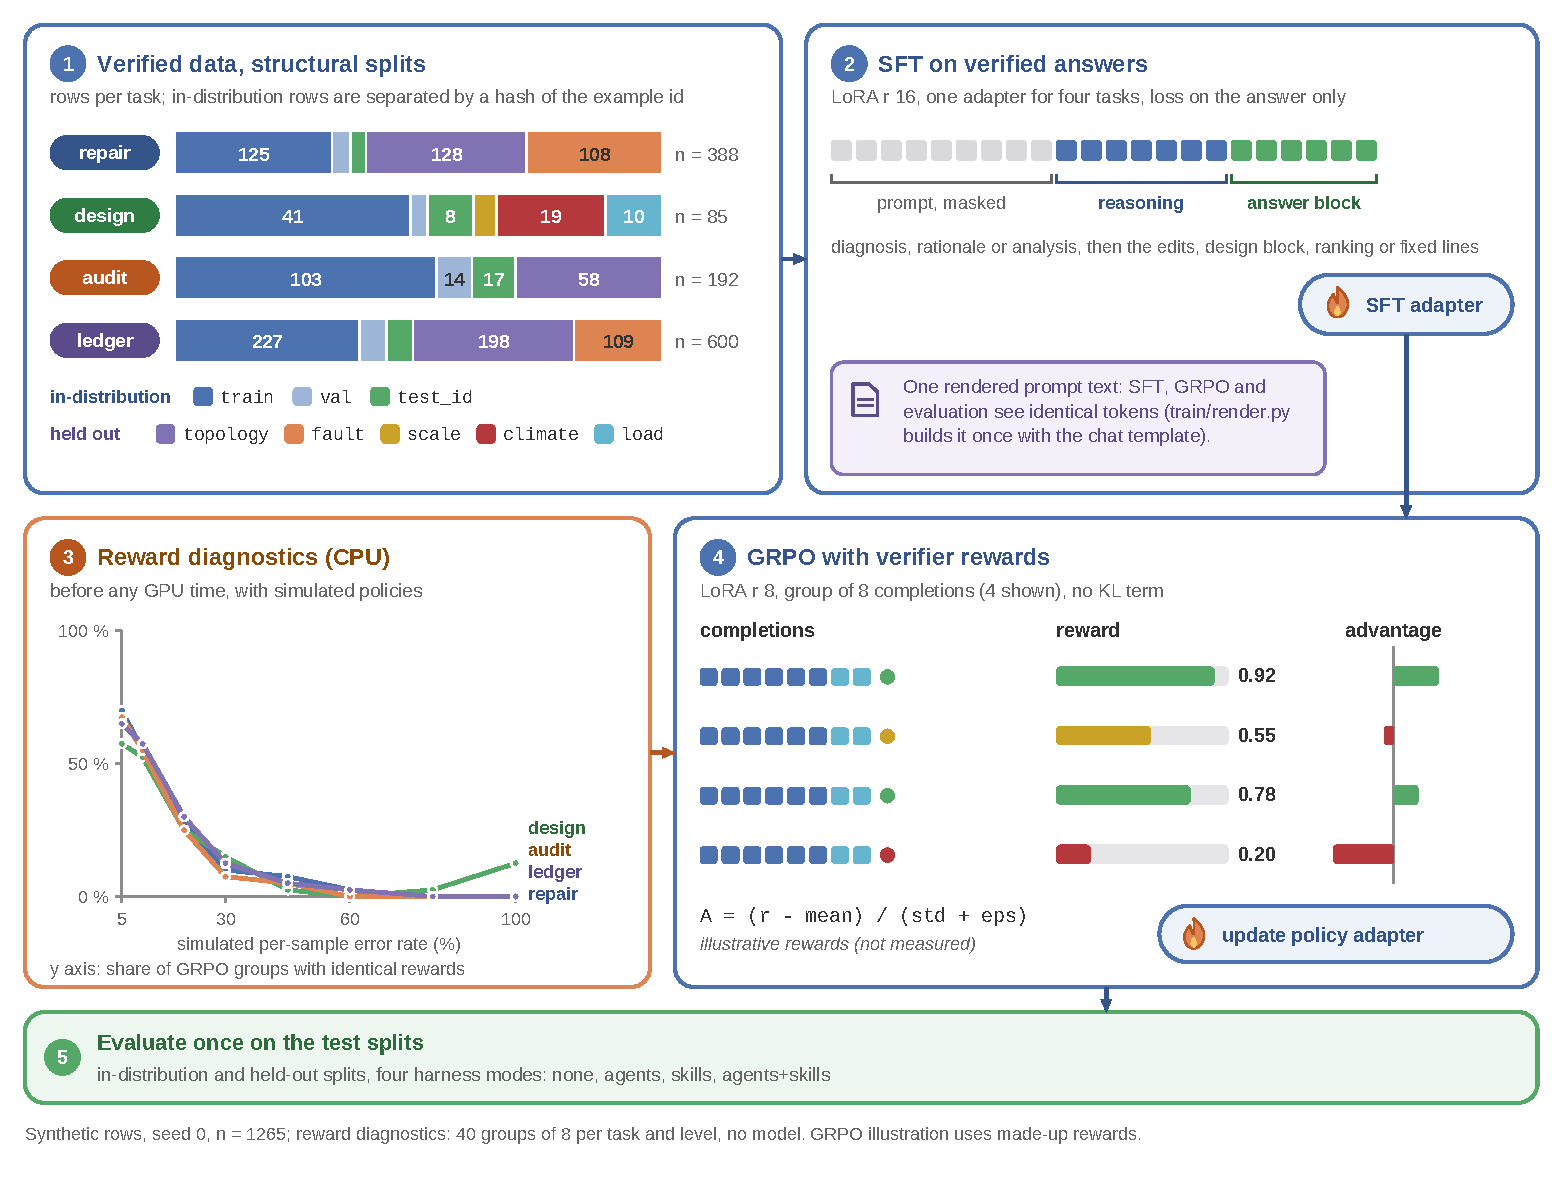
\includegraphics[width=\linewidth]{figures/pdf/fig_training.pdf}
\caption{Planned training pipeline and splits (pre-registered; no training has run). Tool rows use one compact harness and the plain A-slice uses the plain prompt; failure notes are added, prompts above \val{corp.max_prompt_chars} characters and \val{corp.max_prompt_tokens} tokens are dropped and counted (never truncated), and verifier-accepted frontier tool-using CoT traces are kept as SFT completions. The plan is SFT on two data-parallel ranks in fp16 with LoRA, merge, and one joint GRPO run with group sizes k = 4, 8 and 16 (distinct checkpoint paths, four prompts per step, $\mathrm{grad\_accum}=k$); reward diagnostics run on the CPU first, and evaluation is planned on the frozen \texttt{heldout\_v2} test set (the 214-id \texttt{heldout} is dev) over frontier zero-shot and harness replays, base 4B/9B, our SFT and GRPO k4/k8/k16, and other-LLM stand-in arms. Lower panel: rows per split of the ground-truth datasets (\val{split.total} rows from \texttt{data/processed} plus the diagram catalog \texttt{data/processed\_arch}, where \val{corp.arch_kept} of \val{corp.arch_requested} requested injections were kept). The decided corpus sizes are 4,800 tool rows per task family and a 1,600-row A-slice, both built; the remaining datagen item is the frontier chain-of-thought campaign (\cref{sec:datagenstatus}). Trained-model evaluation results are pending. Data: \texttt{assets/splits.json}, \texttt{assets/corpus.json} (simulation, synthetic rows).}
\label{fig:fig_training}
\end{figure}

\subsection{Training corpus}\label{sec:corpus}\label{sec:corpusstatus}

A model that sees one wording of one fault on one diagram can memorize it. The corpus therefore varies several axes at once, and every row is
accepted by the physics tool suite, not by its appearance. It has four sources, kept distinguishable by a source tag, plus the harness text (\cref{tab:corpus}). \Cref{fig:fig_corpus} shows the composition.

\paragraph{Current corpus status (datagen complete except frontier CoT).}
The corpus-side datagen is built and audited. The deterministic tool corpora hold 4,800 rows per task family (600 plants $\times$ 2 variants (direct, recover) $\times$ 4 tasks) with real physics tool results and 100\% verifier acceptance; the plain single-turn A-slice is complete at 1,600 rows ($=\mathrm{round}(4{,}800\times0.3333)$, 400 per task), held-out-excluded and re-measured with the real Qwen3.5 tokenizer. Every tool row is rendered with one compact harness text and the plain prompt is used only for the A-slice. Rows carry \texttt{easy}/\texttt{medium}/\texttt{hard} in equal thirds within each task, derived from the documented per-task size measure in \texttt{thermo\_agent/synth/tiers.py}, with the remainder to the higher tier and exact counts in the manifests. The test set \texttt{heldout\_v2} is frozen (3,476 scored rows in 12 cells, equal thirds per task, contamination scan PASS with zero overlap; \cref{sec:protocol}). Per-row provenance states deterministic vs AI and the exact model id on AI rows, and the token gate (8,192, measured with the real Qwen3.5 tokenizer) drops over-gate rows and counts them rather than truncating. The one open datagen item is the frontier harness chain-of-thought campaign (\cref{sec:datagenstatus}). No corpus has been used for training: no SFT step, GRPO step or checkpoint exists.

\begin{figure}[tbp]
\centering
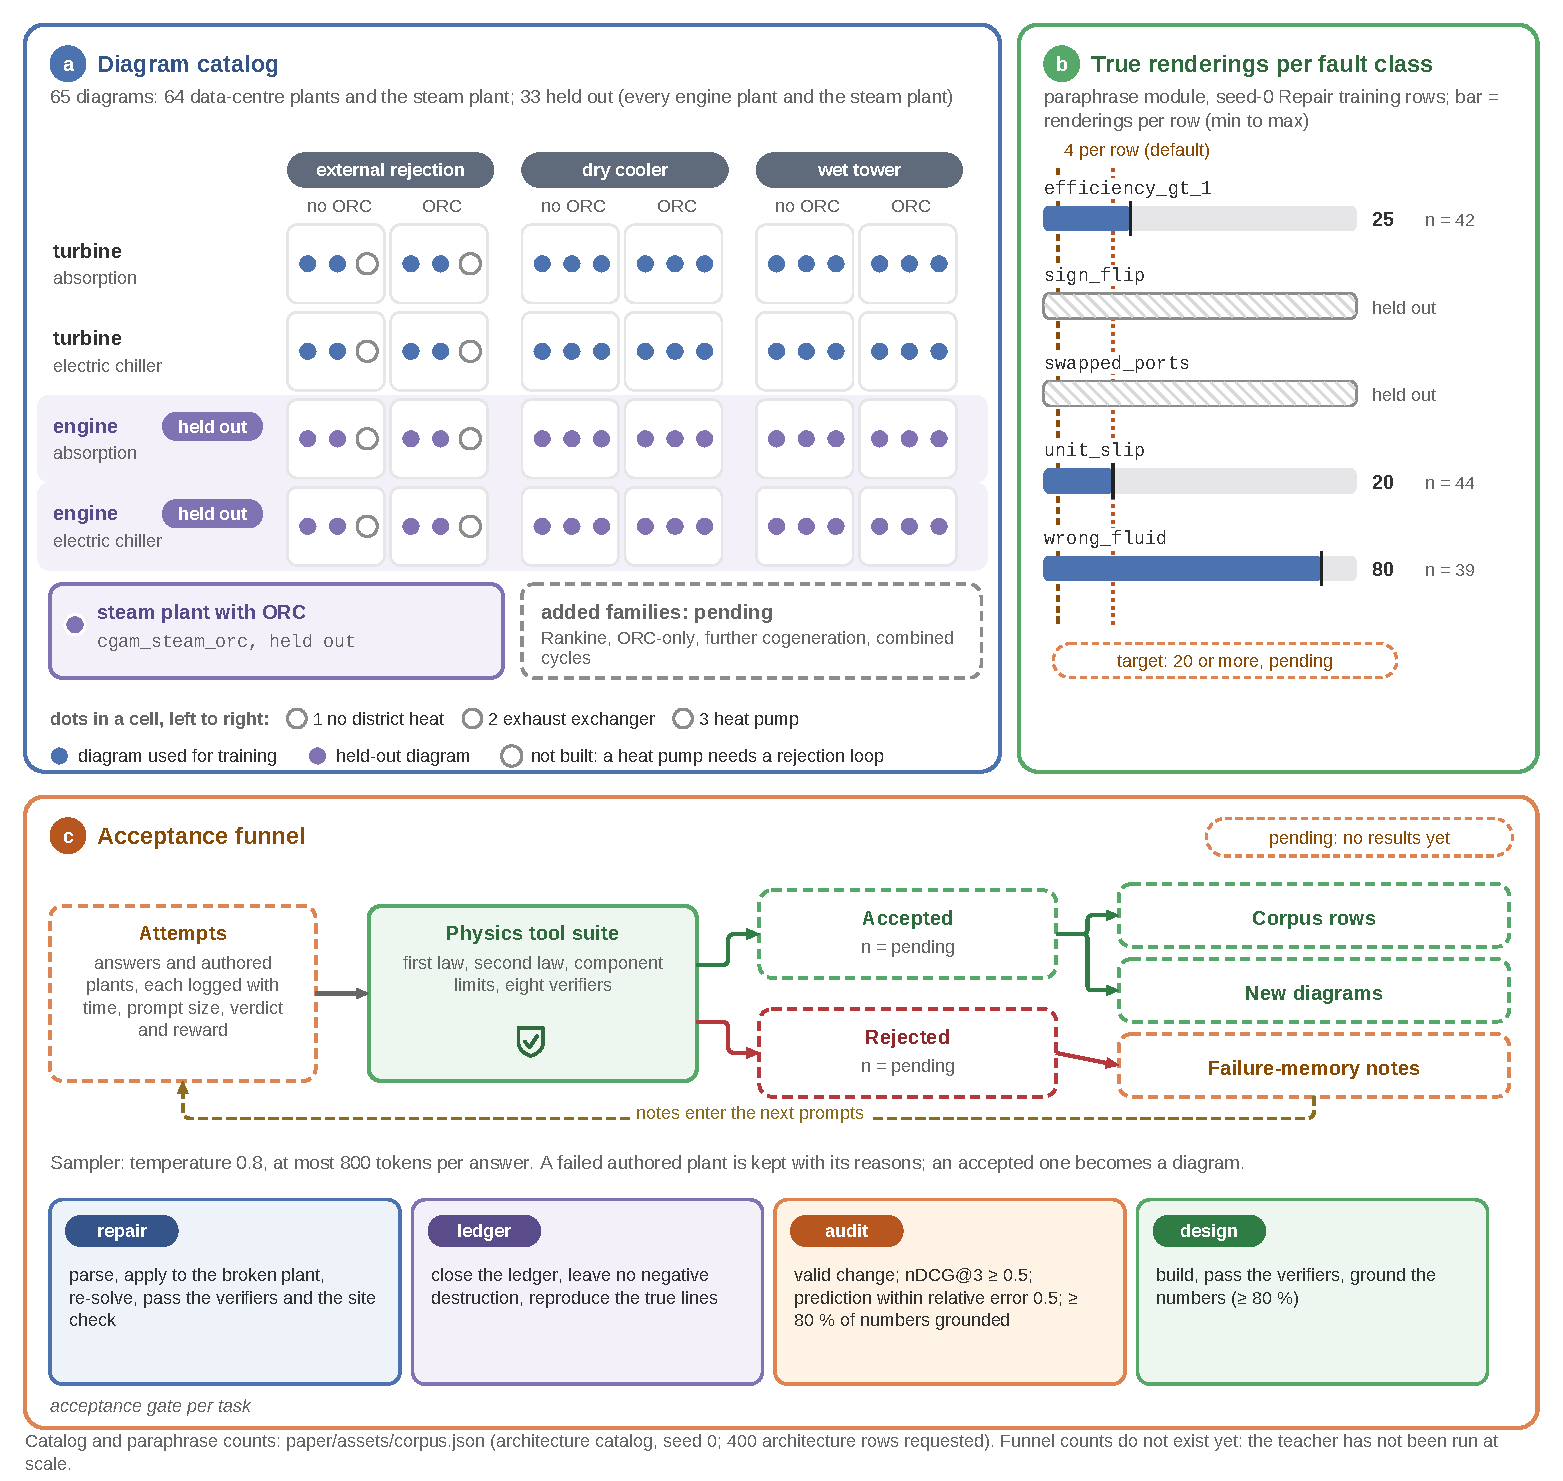
\includegraphics[width=\linewidth]{figures/pdf/fig_corpus.pdf}
\caption{Corpus composition. (a) The diagram catalog (\val{corp.n_arch} diagrams at the seed-0 sample): prime mover and cooling against rejection and ORC, with the district-heat options as dots; the \val{corp.n_held} held-out diagrams are the steam plant and the gas engines with the ideal-rejection boundary. (b) True renderings per fault class in the paraphrase module (\val{corp.var_min} to \val{corp.var_max}), with the held-out fault classes hatched. (c) The acceptance funnel from attempts through the physics tool suite to corpus rows, new diagrams and failure-memory notes, drawn as an empty skeleton: the teacher paths have not been run at scale. Data: \texttt{assets/corpus.json} (simulation).}
\label{fig:fig_corpus}
\end{figure}

\begin{table}[tbp]
\centering\small\renewcommand{\arraystretch}{1.15}
\begin{tabular}{@{}p{2.7cm}p{3.2cm}p{3.7cm}p{1.9cm}p{3.1cm}@{}}
\toprule
Source & Produced by & Gate & Varies & Role in training \\
\midrule
Ground truth with paraphrases & simulator and fault injectors & correct by construction (the original plant is restored) & wording & SFT rows with a fully known answer \\
Architecture corpus & catalog of labeled diagrams (\val{corp.n_arch} at the seed-0 sample) & the solver or the verifiers detect the injected fault & diagram & SFT rows on many system layouts; whole diagrams held out \\
Teacher answers & frontier models through Kaggle's model access & the physics tool suite accepts the answer & reasoning and edits & SFT rows with a second style of reasoning \\
Teacher-authored diagrams & the same models, writing plants in the plant language & the plant solves and passes the verifiers & diagram & new plants for the fault, ledger and audit rows \\
Hindsight memory & accepted and rejected attempts, compared with the ground-truth pattern & notes name a class of mistake or a working pattern, not the answer & what to recheck, and what passed before & success and failure notes in prompts at training and inference \\
Harness text & compact \texttt{AGENTS.md} and one selected skill & none & prompt text & one text for every tool row; plain prompt only for the A-slice \\
\bottomrule
\end{tabular}
\caption{Sources of the training corpus. The corpus builder combines them and records, per source, the rows kept and the prompts dropped.}
\label{tab:corpus}
\end{table}

\paragraph{Ground truth with paraphrases.}
Every Repair row is rendered from the injected fault and its inverse patch. For the seed-0 training rows, the paraphrase module has between \val{corp.var_min} and \val{corp.var_max} true renderings per fault class;
a row picks one by a hash of its identifier, and the corpus builder emits several per row (default \val{corp.variants_default}). Wording varies while the content cannot drift, because every rendering comes from the same facts.
The final corpus uses \val{corp.variants_default} variants per ground-truth Repair row, which is the whole pool of the sparsest fault class and a fifth of the largest, and the training split exercises \val{corp.var_max} distinct renderings across the classes. Ledger, Audit and Design rows vary through sampled plants, faults and sites, with one rendering each, because a paraphrase of a ledger row would only repeat the same site.

\paragraph{Architecture corpus.}
The catalog is a list of labeled plant diagrams: the data-center cogeneration plants (gas turbine or gas engine, absorption or electric cooling, ideal, dry or wet rejection, ORC bottoming on the remaining exhaust and district heat off the exhaust or a heat pump; a heat pump needs a rejection loop, so the eight combinations that lack one are skipped), and the steam-and-HRSG plant with an ORC, \texttt{cgam\_steam\_orc}.
At the seed-0 sample, the catalog has \val{corp.n_arch} diagrams, of which \val{corp.n_dc} are data-center plants; \val{corp.n_turbine} have a gas turbine and \val{corp.n_engine} a gas engine, \val{corp.n_orc} carry an ORC and \val{corp.n_heat} supply district heat.
Whole diagrams are held out, not single parameters: the eight gas-engine plants with the ideal-rejection boundary and the steam plant are in the held-out-topology split, so the model is tested on two layout combinations it never saw, while ORC, gas engines with dry or wet rejection, gas turbines and district heat all train.
The architecture generator was asked for \val{corp.arch_requested} fault injections over the catalog and kept \val{corp.arch_kept} (\val{corp.arch_kept_pct}\%) whose fault the solver or the verifiers detect; \val{corp.arch_distinct.train} distinct diagrams are in its training split and \val{corp.arch_distinct.test_ood_topology} in the held-out-topology split.

\paragraph{Teacher answers.}
Frontier models propose answers to the same prompts that the small model will see, with the harness text and retrieved memory notes in the prompt. They are reached through Kaggle's own model access (Kaggle Benchmarks and the Kaggle command line). The current campaign authorizes only \texttt{gpt-6-luna} and \texttt{claude-haiku-5-5}; each has completed a five-row proof (5/5 accepted) and one 100-row batch, with the journals at the local gate/ingest/audit stage. Luna uses a tools-without-reasoning setting (a documented deviation: the API rejects tools together with reasoning for luna). The target is thousands of verifier-accepted harness-CoT traces with no cap on traces, per-model counts, cost or rows, in equal thirds across \texttt{easy}/\texttt{medium}/\texttt{hard}; the old 72-cell premium target is discarded. Premium models (\texttt{gpt-6.2-sol}, \texttt{claude-sonnet-5-5}, \texttt{claude-opus-5-5-default}, \texttt{gemini-4-argon}) and \texttt{gemini-3.8-flash}/\texttt{gemini-3.5-flash-lite} are not to be run; no traces, costs or scores exist for them. Every file that reaches Kaggle goes through the private HF corpus repo \texttt{Reza-Nadimi/thermo-agent-corpora} into one Kaggle dataset: no local data is uploaded to Kaggle, credentials live only in the repository-root \texttt{.env}, and one generic notebook (\texttt{kaggle\_model\_runner.py}) serves every workflow. Prompts are exported to a file, run in a notebook, and the completions are downloaded and validated locally. An early, superseded pilot left a small number of legacy traces in the provenance ledger; they are not part of the current authorized luna/haiku campaign and no performance claim is made from them. For the current objective the frontier model runs inside a LangGraph harness where it can call the real physics tools, read numeric feedback and revise; a verifier-accepted trace is stored with its full reasoning, tool calls and revisions as the SFT completion, so the student learns tool use rather than only the final answer. The five exposed tools and their one-line contracts are: \texttt{inspect\_plant} --- solve / verify the plant or ledger as given, with no candidate argument; \texttt{first\_law\_check} --- mass / energy residuals (kg/s, W), convergence, tear residual and unit / range flags; \texttt{second\_law\_check} --- exergy destruction (MW), closure, non-negativity and Carnot / COP limits; \texttt{validity\_check} --- validity, failed checks, pinch approach and ranges; \texttt{solve\_plant} --- the full stream table ($T$, $P$, $h$, $s$, exergy). Grading / acceptance is deliberately not exposed as a tool (P0-8): the model receives only physics feedback and must decide for itself when its answer is acceptable.
The sampler records every attempt, accepted or not, with its timestamp, elapsed time, prompt size, verdict and reward, and a resumed run does not spend quota again on attempts already logged. Sampling is at temperature \val{corp.samp_temperature} with at most \val{corp.samp_max_tokens} tokens. The teacher never sees the ground truth.
An attempt becomes a training row only if the tool suite accepts it:
a Repair answer must parse, apply to the broken plant, re-solve and pass the verifiers and the site check; a Ledger answer must close the ledger, leave no negative destruction and reproduce the true lines;
an Audit answer needs a valid change, a ranking with nDCG@3 of at least \val{corp.ndcg_min}, a prediction within a relative error of \val{corp.pred_err_max}, and at least \val{corp.ground_min_pct}\% of the numbers in its analysis grounded in the plant; a Design answer must build, pass the verifiers and ground its numbers to the same share.
These checks are the verifiers of \cref{tab:verifiers}: balances, the first and second laws, the temperature cross in exchangers such as a preheater or an HRSG, and the limits on each component.
Attempts are not discarded. A rejected attempt becomes a failure note that names a class of mistake; an accepted attempt becomes a success note that names the working pattern and the edits that passed the verifiers. Both are retrievable, so the prompt carries what to avoid and what has worked.

\paragraph{Multi-turn tool-using trajectories.}
Training uses genuine multi-turn tool use for both teacher and student: the model reasons, emits a tool call, receives the real numeric result of a physics tool, reads it, revises, and calls again, for up to \texttt{DEFAULT\_MAX\_ROUNDS} = 6 rounds, before returning the final answer (decision D4 applies the same six rounds to trace generation, training and frontier H evaluation). A stored tool-using completion has the shape reason --- \texttt{<tool\_call>}/\texttt{<tool\_result>} pair --- revision --- another call, repeated, and always ends with the verifier-accepted answer; the frontier traces collected so far contain at most five assistant turns under the earlier harness, while the decided compact harness uses six. Tool results are environment output and never a training target: SFT masks every \texttt{<tool\_result>} span and the Qwen-native \texttt{<tool\_response>} form, tags included, to $-100$, while reasoning, calls and the final answer stay trainable. A row is tagged as tool-using only when its stored completion actually contains tool turns; a harness record with no calls is not relabelled just because it carried a trajectory.

\paragraph{Teacher-authored diagrams.}
The teacher is also asked to write whole plants in the plant language, for a stated purpose such as a cogeneration plant for a given site or a Rankine cycle with a given steam condition. The solver and the verifiers check each plant: it must solve, close every balance, show no temperature cross
and keep every component inside its limits, and a plant that fails is kept with its reasons. An accepted plant becomes a new diagram. The fault injectors, the ledger program and the audit procedure then turn it into Repair, Ledger and Audit rows with a known answer, and the teacher can be sampled on those rows in turn. The model therefore reads diagrams that the catalog builders did not write
(none have been accepted at the time of writing, so this share is currently empty).

\paragraph{Hindsight success-and-failure memory.}
Each rejected attempt becomes a short note: the task, the fault class, the diagram, the symptom that the verifiers reported, the class of the mistake and the correct pattern from the ground truth. Notes are retrieved by lexical token overlap with the current plant text,
with a small boost when the query names the note's fault class or diagram, a minimum score of \val{corp.mem_min_score} and a limit of \val{corp.k_memory} notes, and any note mined from the same record is excluded. Notes describe classes of mistakes and never the answer to the current row;
they are appended after the harness text so that the model reads the usual failure modes for a plant of this kind and rechecks its answer. The sampler writes new notes into a shared memory directory, so the next prompt and the student read them. The retrieval is lexical and not an embedding search. A check that notes mined from training records cannot leak information into a held-out split is planned and has not yet passed.

\paragraph{Compact served memory.}
The ledger on disk is for our analysis; what is served to the model is a short recap, one line per retrieved note, each marked \texttt{OK} (verifier-accepted) or \texttt{FAIL} (verifier-rejected) and pairing a fault class with a reusable fix pattern. Bookkeeping is deliberately dropped before prompting: model and provider identifiers, timestamps, cost, token counts, latency, record identifiers, architecture and the raw checker log do not reach the model. Hand-written seed method notes (\texttt{source: seed:method}) are capped to at most one per served block, with the freed slots backfilled by verifier-mined notes, so generic guidance cannot crowd out plant-specific evidence. For one representative repair query at $k=3$, the rendered block measured 159 tokens with the Qwen3.5-4B tokenizer (76 words).

\paragraph{Combination.}
The corpus builder merges the sources into one file per task and split, renders every tool row with the compact harness and leaves the plain A-slice in its plain single-turn form, adds retrieved notes, and measures every prompt with the model's own tokenizer, dropping rows above \val{corp.max_prompt_chars} characters or \val{corp.max_prompt_tokens} tokens so that no row is silently truncated to fit the sequence length. It writes a report of dropped prompts, rows per source and a check of the expert reward. A second pass re-reads the written files, compares every row count with that report and checks that no identifier crosses a split, so a corpus that was moved or half-copied fails before training starts.
The ground-truth source corpus has \val{corp.rows} rows, \val{corp.rows_train} of them in the training split: Repair \val{corp.rows.repair.train}, Ledger \val{corp.rows.ledger.train}, Audit \val{corp.rows.audit.train} and Design \val{corp.rows.design.train}. The decided training mix (\texttt{sft\_mix\_h}) is the 4,800-row deterministic tool corpus plus the 1,600-row plain A-slice, with verifier-accepted frontier traces added first as they arrive. The teacher-authored share is empty at the time of writing: frontier harness-CoT datagen is still in progress (luna and haiku proofs plus one 100-row batch each) and has yielded accepted tool traces, not a corpus of teacher-authored diagrams.

\paragraph{Provenance.}
Every training row must state whether it is deterministic or AI-generated, and if AI-generated which model produced it. Deterministic rows are derived from ground truth by the simulator and the fault injectors, not written by a language model; frontier rows carry the exact model id and journal path. This tag is part of the row schema and is checked before a corpus is accepted.

\begin{table}[tbp]
\centering
\begingroup\small\renewcommand{\arraystretch}{1.15}
\begin{tabular}{@{}p{2.3cm}p{2.6cm}p{2.6cm}p{3.1cm}p{3.1cm}@{}}
\toprule
Task & Teacher attempts & Accepted (share) & Rejected, kept as notes & Distinct architectures accepted \\
\midrule
Repair & \todo{pending} & \todo{pending} & \todo{pending} & \todo{pending} \\
Ledger repair & \todo{pending} & \todo{pending} & \todo{pending} & \todo{pending} \\
Audit & \todo{pending} & \todo{pending} & \todo{pending} & \todo{pending} \\
Design & \todo{pending} & \todo{pending} & \todo{pending} & \todo{pending} \\
\bottomrule
\end{tabular}\endgroup

\caption{Teacher acceptance statistics, to be filled once the campaign completes. Frontier harness-CoT datagen is in progress with two authorized budget models (a five-row proof and one 100-row batch each); no model has been trained or evaluated, so the campaign-wide cells remain pending.}
\label{tab:corpusstatus}
\end{table}

\subsection{Training}\label{sec:training}

\paragraph{Stage 1: supervised fine-tuning.}
Qwen3.5-4B is fine-tuned with LoRA on the combined corpus of \cref{sec:corpus}, with one adapter for all four tasks. Thinking is enabled (\texttt{enable\_thinking=True}) in training, GRPO and evaluation. Prompts are rendered identically in all three, as plain prompt and completion text, so that no template mismatch arises between training and
inference. Supervised fine-tuning comes first because verifiable rewards are sparse for a policy that never succeeds \citep{lambert2024tulu3}. The maximum length is \val{tr.sft_len} tokens, and a prompt that is too long is dropped and counted, never truncated.
The planned SFT settings (decisions A1--A10, B1--B7) are learning rate $10^{-4}$, at most three epochs with early stopping after three evaluations without validation-loss improvement (best checkpoint loaded at the end), a cosine schedule with warmup ratio 0.05, weight decay 0, AdamW, seed 0, gradient clipping 1.0, LoRA rank 32 / alpha 64 / dropout 0.05 on all linear layers in float16, an effective batch of $2\times8\times2=32$ sequences per step, and save/evaluate every 50 steps. The training corpus is the \texttt{sft\_mix\_h} mix of the plain A-slice and the compact-harness tool rows. None of this has been run.

\paragraph{Stage 2: GRPO.}
The best SFT adapter is merged, and one joint GRPO run over all four tasks starts from the merged policy (\texttt{runs/sft\_merged}) with a new rank-8 / alpha-16 LoRA adapter. Completion sampling uses temperature 1.0, top-p 1.0, top-k off, no penalties, and beta 0 (no reference model); the loss is DAPO \citep{yu2025dapo} with group-normalized rewards and truncated completions masked. The reward is the weighted channel sum of \cref{tab:tasks}, dispatched by each prompt's task; prompts are sampled uniformly over task by tier. The maximum completion length is 4,096 tokens for the whole multi-turn completion, with at most six tool-calling iterations; a 320-token budget cannot hold a tool trace, and if dev truncation exceeds 10\% the limit is raised to 6,144. We plan group sizes $k\in\{4,8,16\}$ with four prompts per optimizer step, so $\mathrm{grad\_accum}=k$ on two GPUs (16, 32 and 64 sequences per step); all three use the same step count and seed 0. Zero-variance groups are logged, and the run stops if their share exceeds 50\% for ten consecutive logs. These settings (decisions C1--C10) are planned and have not been run.

\paragraph{Data parallelism.}
Training targets two T4 GPUs on one host, joined by PCIe without NVLink. The base model is replicated on each GPU (distributed data parallel), so that only the LoRA gradients, tens of megabytes in fp16, cross the link, once per optimizer step; sharding the 4B weights would move about 8~GB per step over the same link.
The T4 has no bf16 kernels, so the model runs in fp16 with dynamic loss scaling, gradient clipping and fp32 accumulation in matmuls, and 4-bit weights are not used. The effective batch is \val{tr.sft_batch_eff} sequences for SFT and \val{tr.grpo_batch_eff} prompts of \val{tr.group} completions for GRPO (\cref{tab:training}).
The code is written against TRL \citep{vonwerra2020trl} and has not been run on a GPU; loading the model, the library's argument names, fp16 overflow, merging and generation-length cutoffs are the known risks.

\begin{table}[tbp]
\centering
\begingroup\small\renewcommand{\arraystretch}{1.12}
\begin{tabular}{@{}p{4.2cm}p{5.4cm}p{5.6cm}@{}}
\toprule
 & Stage 1: SFT & Stage 2: GRPO \\
\midrule
Base model & \texttt{Qwen/Qwen3.5-4B} & \texttt{Qwen/Qwen3.5-4B} \\
Method & LoRA SFT, all tasks in one adapter & GRPO per task on the merged SFT model \\
Precision and parallelism & fp16 LoRA, DDP over 2 ranks (2 T4), no 4-bit & fp16 LoRA, DDP over 2 ranks, no 4-bit \\
LoRA rank / alpha / dropout & 16 / 32 / 0.05 & 8 / 16 / 0.05 \\
Target modules & all-linear & all-linear \\
Learning rate & 0.0002 & 5e-05 \\
Epochs or steps & 2 epochs & 300 steps (maximum) \\
Maximum length (tokens) & 4096 & completion 320 \\
Batch per device / accumulation / ranks & 2 / 8 / 2 & 4 / 2 / 2 \\
Effective batch & 32 sequences & 16 prompts, 4 completions each \\
Group size / temperature & -- & 4 / 1 \\
Gradient clipping & max norm 1 & max norm 1 \\
Loss & causal LM, completion tokens only & dapo-style, KL coefficient 0, truncated completions masked \\
Prompt rendering & tokenizer generation prompt, thinking disabled & same text as SFT and evaluation \\
\bottomrule
\end{tabular}\endgroup

\caption{Training settings, read from \texttt{train/config.py} (ranks from the dual-T4 recipe of the repository). None of this has been run on a GPU.}
\label{tab:training}
\end{table}

\paragraph{Reward diagnostics.}
Before any GPU time, each reward is probed with simulated policies that return the expert answer with probability $1-e$ and a damaged answer otherwise. For groups of
\val{rd.G} completions the diagnostic reports the share of groups whose rewards are all equal; the training group is \val{tr.group}, so the diagnostic is run at that size and, for comparison, at 8, where equal groups are less frequent. Such groups carry no gradient under group-normalized advantages, so they indicate the error rate below
which GRPO stops being informative for a task (\cref{sec:rewarddiag}).

\subsection{Agent harness and memory}\label{sec:harness}

The harness is text added to the system message. An \texttt{AGENTS.md} file holds conventions, verifier meanings, how to read solver errors and the answer formats; \val{env.n_skills} skills cover the gas
engine, heat rejector, absorption chiller, ORC bottoming, heat pump and district heat, the exergy audit, the design catalog and the exergy ledger. The port and parameter sections of the
skills are generated from the component registry, and a test fails if they drift from it. There are four harness modes: none, \texttt{AGENTS.md}, skills, and both. In the skill modes the bodies of the selected skills
are appended to the system message (they are not loaded on demand); a component skill is selected when its component appears in the plant. When there is no plant yet, as in Design, only the task's own skill (the design catalog, which lists the components and their parameters) is given, because every component skill at once would push a Design or Ledger prompt past the length limit.
The hindsight memory (\cref{sec:corpus}) is a separate layer that can be switched on independently of the mode, in the SFT prompts, in the GRPO rollouts and in evaluation, so that the harness ablation stays a four-mode comparison and memory adds a second factor.
The planned ablation holds the gas engine out of the training diagrams, so that its skill is its only description (\cref{sec:experiments}).

\paragraph{Compact harness.}
For every arm --- trace generation, training and frontier H evaluation --- the harness is one compact text of at most 2,500 tokens measured with the real Qwen3.5 tokenizer (decisions J2/J3): it keeps the tool contract, output tags, the failure checklist and the one selected skill, and drops prose examples and non-selected skills. The sequence gate stays at 8,192 tokens; over-gate rows are dropped and counted, never truncated. The harness runs six tool rounds with a memory limit of $k=3$ notes (decisions D4/D5). The compact harness text is built, audited and used for the frontier CoT traces; no training or evaluation arm has been run under any harness and no checkpoint exists.

\begin{figure}[tbp]
\centering
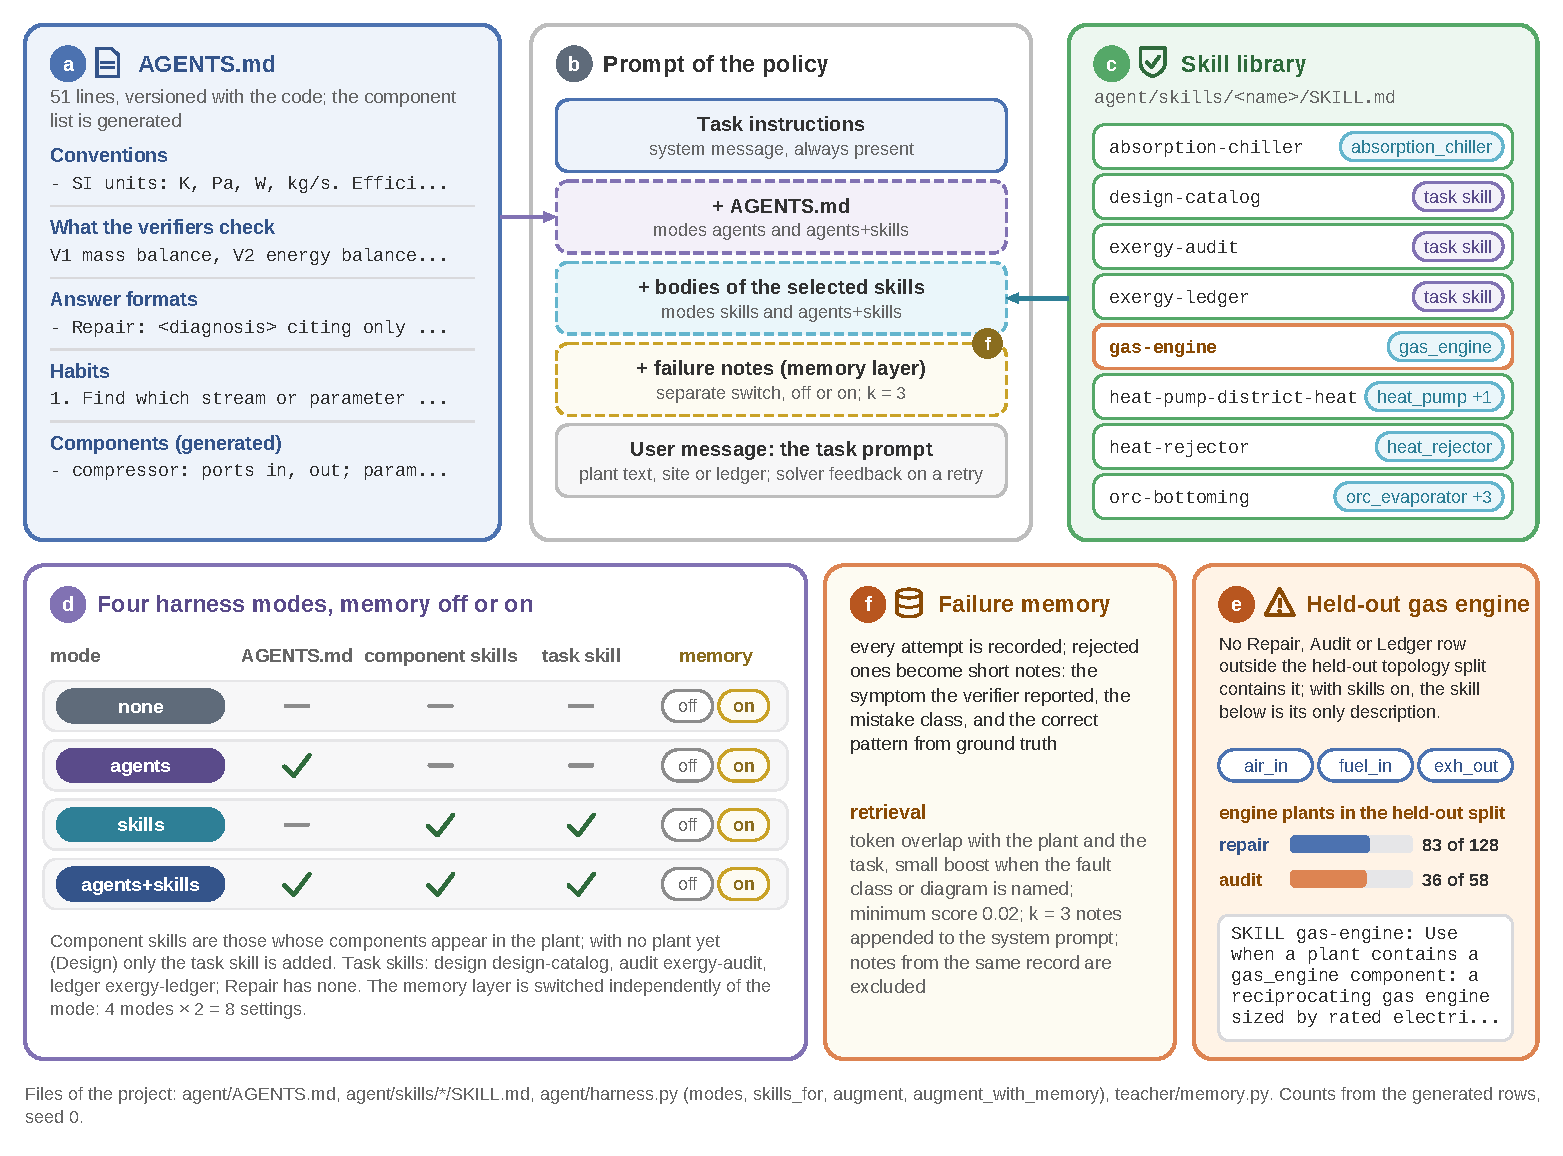
\includegraphics[width=\linewidth]{figures/pdf/fig_harness.pdf}
\caption{Harness and memory. \texttt{AGENTS.md} and the skill library (\val{env.n_skills} skills) are generated from the component registry; four harness modes add none, \texttt{AGENTS.md}, skills or both to the system message, and the memory layer (lexical retrieval of success and failure notes, at most \val{corp.k_memory} notes, notes from the same record excluded) is a separate switch, giving eight settings. With no plant (Design) only the task skill is added. The gas engine is the component held out of training. Data: \texttt{assets/harness.json}, \texttt{assets/corpus.json}.}
\label{fig:fig_harness}
\end{figure}

\section{Experiments}\label{sec:experiments}

Everything in this section that is a number was measured on the CPU with the project code and fixed seeds, on small samples, and
every sample size is stated. All measured results are simulation-driven. No language model has been trained or evaluated: no SFT or GRPO checkpoint exists and no model arm has been scored. The frontier zero-shot and harness arms are replays of saved answers from \texttt{data/kaggle\_datasets/thermo-agent-eval-replays/}, scored through the same verifiers. The model results and ablations (\cref{sec:modelresults,sec:ablations}) are skeletons whose cells are pending, and every protocol value below is pre-registered rather than measured. Datagen is not complete (\cref{sec:datagenstatus}), so by Reza's directive of 2026-11-19 training has not started. The frozen test set is \texttt{data/heldout\_v2}; the 214-id \texttt{data/heldout} is the dev set used for tuning only.

\subsection{Pre-registered protocol}\label{sec:protocol}

\paragraph{Models and harness.}
We evaluate the arms of decision F4. (i) Base Qwen3.5-4B and Qwen3.5-9B; (ii) our SFT checkpoint; (iii) our GRPO checkpoints at $k=4,8,16$, each from the merged SFT policy. Each of these appears in two modes: Z (plain prompt, no tools) and H (compact harness, tools and memory). (iv) Frontier zero-shot (Z) and frontier harness (H) arms, which are replays of saved answers from \texttt{data/kaggle\_datasets/thermo-agent-eval-replays/} through the same verifiers and prompt rows; a replay is evidence for that saved answer set only. (v) Other-LLM stand-in arms, plus the non-model baselines of \cref{sec:baselines}. The old \texttt{sft none} guard is replaced by this table; the two modes of a given model are scored on identical rows, so the harness effect is a paired comparison. Every arm sees the same rows of the frozen \texttt{heldout\_v2} test set and the same answer budget. Frontier models are reached through Kaggle's model access (not a local API); their saved answers are replayed, and Kaggle reports the token cost of each call. The mode and tool-access axes are recorded as columns in \cref{tab:comparison}. No arm has been scored yet; the SFT-tools-only versus SFT-mix comparison of decision F5 is deferred until the main table exists.

\paragraph{Decoding, attempts and budgets.}
Decoding is pre-registered as follows (all local arms identical). The primary condition is greedy decoding (\texttt{do\_sample=False}, repetition penalty 1.0, no presence penalty). A secondary pass@8 uses temperature 0.6, top-p 0.95, top-k 20, min-p 0 and seeds 0--7, again without repetition or presence penalties; these are Qwen's published thinking-mode precise-task settings (the general-chat presence penalty of 1.5 is rejected because structured output legitimately repeats unit tokens, ids and tool arguments). Frontier hosted models use provider defaults, which are recorded per run. The harness runs up to six tool rounds with at most eight tool calls; per-turn generation is capped at 4,096 new tokens, with a sequence gate of 8,192 tokens and over-gate rows dropped rather than truncated. Cost is counted in solver calls (Repair) or design evaluations (Design). Design also has an anytime protocol: the model is told the fuel of each valid design and may
refine, and we record the best gap to the reference after $b$ design evaluations, to compare with enumeration, random search and
enumerate-then-polish at equal budgets. None of these conditions has been run.

\paragraph{Metrics.}
Repair: success (the repaired plant is valid and serves the site), first-turn success, exact restoration on deducible faults, and mean solver calls. Design: valid share, share within 1\% of the reference, mean fuel gap, mean
evaluations. Audit: ranking score, validity of the change, gain and prediction score. Ledger repair: exactness, closure and the share of rows with all lines correct.

\paragraph{Statistics.}
Binary outcomes carry Wilson 95\% intervals \citep{wilson1927interval}. Two runs on the same examples are compared with an exact McNemar test for binary
metrics \citep{mcnemar1947}, and with a paired bootstrap interval plus a sign-flip permutation test for other metrics; all comparisons reported together are
Holm-corrected \citep{holm1979}. Per-example results are saved with each report. ThermoQA accuracy before and after training checks for forgetting.

\paragraph{Test set, dev set and tiers.}
The held-out test set is \texttt{data/heldout\_v2}, frozen before any model is scored; \texttt{data/heldout} (214 test ids) is the dev set and is used for tuning only, never reported as a test result. Within each task, rows are split into \texttt{easy}, \texttt{medium} and \texttt{hard} in equal thirds in both the training corpora and \texttt{heldout\_v2}; the tier is a real column derived from a documented per-task size measure (\texttt{thermo\_agent/synth/tiers.py}), never random and never a threshold tuned by the assistant. When a task's rows cannot be cut into exact thirds, the remainder goes to the higher tier and the manifest records the exact counts per task. The target is at least 85 rows per reported cell where a generator can reach it, with any merged cells documented explicitly. All of this is a pre-registered design: no cell has been scored.

\paragraph{Cost accounting and provenance.}
Three costs are reported separately and never merged into one score. Physics cost is solver calls (Repair) or design evaluations (Design); it is measured for every arm by the same evaluator. Model cost is the token count and the price that Kaggle Benchmarks reports for a frontier call (in nanodollars, summed per model in \texttt{reports/frontier\_ingest.json}), plus GPU-hours for our own training and inference. Data cost is the number of ground-truth plants, paraphrases, teacher attempts and accepted rows. Because frontier answers are static replays, their cost is charged once and reused across arms; the report states this instead of implying a fresh call per evaluation. Every result file carries the model id, harness mode, tool-access flag, seed, limit and sample size in its \texttt{meta} block, and the paper tables are generated from those files rather than transcribed.

\paragraph{Qualitative evidence.}
Figures are not hand-drawn illustrations. \Cref{fig:fig_trace_walkthrough} is regenerated from a deterministic selection of real traces -- a fault from the ground-truth corpus, a frontier interaction with recorded tool calls and reasoning (from the 32 accepted traces, replayed), a GRPO group (planned; none has been generated), and the comparison arms (planned) -- with the field schema and source files stored beside the examples. The selection rule is part of the generator, so the same inputs reproduce the same figure; no example is chosen from a model result by hand.

\paragraph{Research questions.}
We fix eight research questions before the runs and state no expected answer to any of them.
\textbf{RQ1:} does a trained model match the success of verifier-guided search on held-out faults with fewer solver calls?
\textbf{RQ2:} how much do the inference text and the physics tools help a frontier model, and how much of our model's behaviour depends on that text?
\textbf{RQ3:} does GRPO add over SFT on tasks where SFT is below about 90\% per-sample accuracy, and on held-out diagrams?
\textbf{RQ4:} do the individual reward channels matter?
\textbf{RQ5:} is there forgetting on ThermoQA?
\textbf{RQ6:} does the varied corpus (paraphrases, the diagram catalog and verified teacher answers) improve success on held-out diagrams over ground-truth traces alone?
\textbf{RQ7:} does retrieving failure notes improve success or the first-attempt acceptance rate, and does it help more than random notes?
\textbf{RQ8:} how close does the trained 4B model come to zero-shot frontier models, frontier models with our harness and tools, and other models, at equal prompts and an equal answer budget?

\subsection{Non-model baselines}\label{sec:baselines}

Non-model baselines set the cost against which a trained model is compared. \Cref{tab:baselines} gives them with sample sizes.

\begin{table}[tbp]
\centering
\begingroup\scriptsize\renewcommand{\arraystretch}{1.15}
\begin{tabular}{@{}p{5.7cm}rp{3.1cm}p{3.1cm}l@{}}
\toprule
Baseline (no language model) & $n$ & Main result (95\% Wilson) & Cost or reference & Seed \\
\midrule
Repair: blind search, in-distribution & 12 & 92\% (65--99) & 174 solver calls & seed 0 \\
Repair: blind search, held-out faults & 108 & 100\% (97--100) & 128 solver calls & seed 0 \\
Repair: blind search, held-out topologies & 128 & 99\% (96--100) & 122 solver calls & seed 0 \\
Design: enumerate defaults, 64 evaluations & 24 & 71\% within 2\% & gap 2.4\% & seed 0 \\
Design: random search, 12 evaluations & 24 & 33\% within 2\% & gap 8.7\% & seed 0 \\
Design: random search, 128 evaluations & 24 & 75\% within 2\% & gap 0.6\% & seed 0 \\
Design: enumerate, then polish, 64 evaluations & 24 & 79\% within 2\% & gap 1.4\% & seed 0 \\
Design: enumerate, then polish, 128 evaluations & 24 & 100\% within 2\% & gap 0.1\% & seed 0 \\
Audit: first-law ranking top-1, in-distribution & 17 & 0\% (0--18) & random 25\% & seed 0 \\
Audit: fixed rule change, in-distribution & 17 & 100\% of best gain & valid 7/17 & seed 0 \\
Audit: first-law ranking top-1, held-out topologies & 58 & 12\% (6--23) & random 32\% & seed 0 \\
Audit: fixed rule change, held-out topologies & 58 & 12\% of best gain & valid 43/58 & seed 0 \\
\bottomrule
\end{tabular}\endgroup

\caption{Non-model baselines on generated rows (simulation, seed 0). Repair: all rows of each split ($n$ is the split size). Design:
\val{des.n_sites} sites, of which \val{des.n_heat_sites} have a heat demand; ``within'' is the share of sites whose best design is within
\val{des.tolerance_pct}\% of the reference. Audit: \val{aud.n_id} in-distribution and \val{aud.n_ood} held-out-topology plants.}
\label{tab:baselines}
\end{table}

\paragraph{Repair.}
A blind search tries single edits on every numeric slot with a fixed set of transforms (scalings, an offset of 273.15, a sign flip, default efficiencies), then structural edits (exchanging two same-fluid
destinations, relabeling a fluid), taking slots named in the verifier output first, and accepts the first plant that solves and passes the hard checks. It does no learning. On the
\val{rep.test_ood_fault.n} held-out-fault rows it repairs \val{rep.test_ood_fault.search_pct}\% (Wilson 95\% interval \val{rep.test_ood_fault.search_lo_pct} to
\val{rep.test_ood_fault.search_hi_pct}\%), on the \val{rep.test_ood_topology.n} held-out-topology rows \val{rep.test_ood_topology.search_pct}\%, and on the \val{rep.test_id.n}
in-distribution rows \val{rep.test_id.search_pct}\% (interval \val{rep.test_id.search_lo_pct} to \val{rep.test_id.search_hi_pct}\%). Doing nothing repairs \val{rep.test_id.noop_pct}\% in each split.
Cost depends on the fault type, pooled over the three splits: \val{rep.f.sign_flip.calls} solver calls on average for \val{rep.f.sign_flip.n} sign flips, \val{rep.f.efficiency_gt_1.calls} for \val{rep.f.efficiency_gt_1.n} efficiencies above 1, \val{rep.f.unit_slip.calls} for
\val{rep.f.unit_slip.n} unit slips, and \val{rep.f.swapped_ports.calls} and \val{rep.f.wrong_fluid.calls} for \val{rep.f.swapped_ports.n} swapped ports and \val{rep.f.wrong_fluid.n} wrong fluids. These are the numbers a trained model must beat to
claim sample efficiency (RQ1). The search finds a valid plant, which need not be the original: it restores the original exactly in \val{rep.test_ood_fault.exact_pct}\% of the held-out-fault rows and \val{rep.test_ood_topology.exact_pct}\% of the held-out-topology rows.

\paragraph{Design.}
\Cref{fig:fig_design_baselines} shows the share of sites whose best design is within \val{des.tolerance_pct}\% of the reference against the number of design evaluations, on \val{des.n_sites} sites (\val{des.split.test_id} in-distribution,
\val{des.split.test_ood_climate} hot-climate, \val{des.split.test_ood_load} high-chilled-fraction and \val{des.split.test_ood_scale} large-scale). Enumerating the defaults takes
\val{des.enum_len_min} evaluations without a heat demand and \val{des.enum_len_max} with one; after \val{des.enum_len_max} evaluations \val{des.enum.b64.within_pct}\% of sites are within the tolerance, at a mean gap of
\val{des.enum.b64.gap_pct}\%. Random search with 128 evaluations (its curve runs to \val{des.random_len}) reaches \val{des.rand.b128.within_pct}\% at a gap of \val{des.rand.b128.gap_pct}\%, and with 12 evaluations it is \val{des.rand.b12.gap_pct}\% from the reference and
valid at \val{des.rand.b12.valid_pct}\% of sites. Enumerate-then-polish is the procedure that defines the reference (\val{des.polish_len_min} to \val{des.polish_len_max} evaluations), so its curve measures the speed of reaching the
reference, not independent quality; it reaches \val{des.pol.b128.within_pct}\% of sites within the tolerance after 128 evaluations. A trained model has to be placed on these axes; its curve is pending.

\begin{figure}[tbp]
\centering
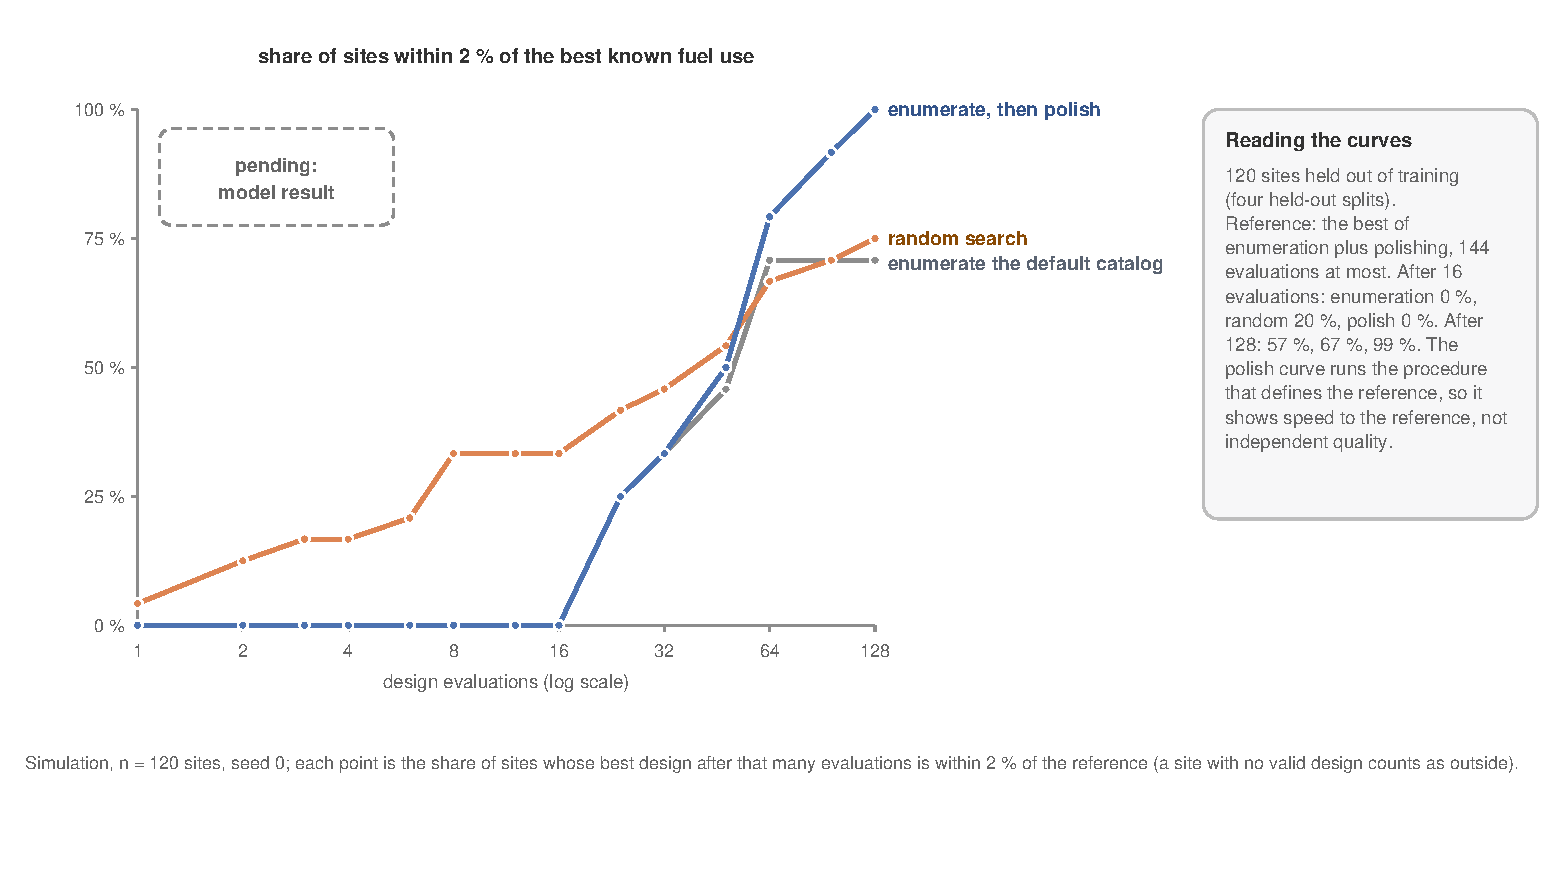
\includegraphics[width=\linewidth]{figures/pdf/fig_design_baselines.pdf}
\caption{Anytime curves of three non-model baselines on \val{des.n_sites} held-out sites (simulation): share of sites whose best design is within
\val{des.tolerance_pct}\% of the reference against the number of design evaluations (logarithmic scale). The reference is the enumerate-then-polish result. The trained-model curve is pending and
shown only as an empty box. Data: \texttt{assets/design\_baselines.json}.}
\label{fig:fig_design_baselines}
\end{figure}

\paragraph{Audit.}
On \val{audb.n_id} in-distribution and \val{audb.n_ood} held-out-topology plants, a fixed rule (raise the turbine inlet temperature by 10\%, or cut the engine loss fraction by 10\%) recovers
\val{audb.rule_gain_id_pct}\% of the best allowed gain on the in-distribution plants, where it is valid for \val{audb.rule_valid_id} of \val{audb.n_id}, and \val{audb.rule_gain_ood_pct}\% on the held-out engine and steam-ORC plants, where it is
valid for \val{audb.rule_valid_ood} of \val{audb.n_ood}. The best allowed change saves a median \val{audb.saving_median_id_pct}\% of fuel in-distribution (range \val{audb.saving_min_id_pct} to \val{audb.saving_max_id_pct}\%) and
\val{audb.saving_median_ood_pct}\% on the held-out topologies (\val{audb.saving_min_ood_pct} to \val{audb.saving_max_ood_pct}\%); exhaustive search over the allowed changes costs about \val{audb.search_evals_id} evaluations. For the prediction channel,
predicting no effect scores \val{audb.pred_zero_id} in-distribution and \val{audb.pred_zero_ood} held out, and predicting the mean relative effect of the other plants scores \val{audb.pred_mean_id} and \val{audb.pred_mean_ood}.

\paragraph{Ledger.}
A program that rebuilds each ledger line from the topology solves every row by construction, so there is no search baseline to report; the finding for this task is the symptom coverage of the faults (\cref{sec:ledger}).

\subsection{Simulator findings}\label{sec:findings}

These findings do not depend on a model. They characterize the simulator and the tasks under the assumed constants of \cref{tab:constants}.

\subsubsection{Feasibility mechanisms of the catalog}\label{sec:feasibility}

We evaluated the catalog at a 20~MW IT load (turbine exhaust about \val{mech.turbine_exhaust_K}~K, engine exhaust about \val{mech.engine_exhaust_K}~K), 25\,$^\circ$C ambient, 50\% relative humidity and
chilled water at 18 to 28\,$^\circ$C (\cref{tab:mech}; chilled fraction in steps of 0.05, wet tower, no grid import; one site, one point per entry). Five mechanisms follow.
\begin{itemize}[leftmargin=*,itemsep=1pt]
\item Exhaust-only recovery limits the engine. An engine with absorption cooling is valid up to \val{mech.engine_max_frac_pct}\% of the IT heat on the chilled loop, with a stack at \val{mech.engine_stack_K}~K; at \val{mech.engine_first_fail_pct}\%
the temperature-cross check fails, and at a chilled fraction of 1.0 the exhaust cannot supply the required duty. A turbine carries 100\% of the heat, with the stack still at \val{mech.turbine_100_stack_K}~K.
\item A single-stage ORC cannot use turbine exhaust: with none of the three fluids (valid for \val{mech.orc_turbine_valid} of \val{mech.orc_turbine_n}) can the evaporator accept an exhaust of about \val{mech.turbine_exhaust_K}~K without exceeding the vapor limit while leaving the stack above the floor.
\item On the engine, bottoming helps with the right fluid. Cyclopentane lowers fuel from \val{mech.eng_none_fuel_mw} to \val{mech.eng_cyc_fuel_mw}~MW (\val{mech.eng_cyc_saving_pct}\%) with \val{mech.eng_cyc_orc_net_mw}~MW of net ORC output, and toluene gives \val{mech.eng_toluene_fuel_mw}~MW; R245fa is infeasible because the exhaust is too hot for its vapor limit.
\item Dry rejection fails in heat. At 32\,$^\circ$C ambient an engine with a dry cooler and absorption cooling fails the temperature-cross check, while with a wet tower it is valid at \val{mech.amb305_wet_fuel_mw}~MW.
\item A water limit rules out wet towers: with a site limit of 0.5~kg/s, a wet tower fails the water check (the tower's make-up bound is \val{mech.water_wet_use_kg_s}~kg/s) and the dry-cooler plant is valid.
\end{itemize}

\begin{table}[tbp]
\centering
\begingroup\small\renewcommand{\arraystretch}{1.1}
\begin{tabular}{@{}rll@{}}
\toprule
Chilled fraction & Engine + absorption, wet tower & Turbine + absorption, wet tower \\
\midrule
0.3 & 48.4 MW, stack 667 K & 57.1 MW, stack 748 K \\
0.4 & 48.5 MW, stack 598 K & 57.3 MW, stack 710 K \\
0.5 & 48.7 MW, stack 529 K & 57.5 MW, stack 673 K \\
0.6 & 48.8 MW, stack 459 K & 57.7 MW, stack 635 K \\
0.7 & 49.0 MW, stack 388 K & 57.8 MW, stack 597 K \\
0.8 & infeasible & 58.0 MW, stack 559 K \\
0.9 & infeasible & 58.2 MW, stack 521 K \\
1.0 & infeasible & 58.4 MW, stack 483 K \\
\bottomrule
\end{tabular}\endgroup

\caption{Fuel use and stack temperature of engine and turbine plants with absorption cooling and a wet tower against the share of the IT heat carried by the chilled loop (20~MW IT load,
simulation, $n=2$ plants per row, assumed constants). ``Infeasible'' marks a plant that fails a hard check or cannot be sized. Data: \texttt{assets/mechanisms.json}.}
\label{tab:mech}
\end{table}

\Cref{fig:fig_design_feasibility} extends this to the whole catalog over \val{feas.n_cells} cells (chilled fraction and ambient temperature, \val{feas.n_specs} specifications each). Of the \val{feas.n_cells} cells, \val{feas.n_cells_none} (all at 283~K) have no valid design because the chiller's heat rejection (ambient plus approach)
is not above its evaporator temperature; free cooling is not modeled, so this is a limit of the model and not an engineering infeasibility. In the other \val{feas.n_cells_valid} cells the mean number of valid specifications is \val{feas.mean_valid} of \val{feas.n_specs},
the winners span \val{feas.n_winner_types} distinct configurations, the engine wins in \val{feas.win.engine_absorption} cells with absorption cooling and \val{feas.win.engine_electric} with electric cooling, and the turbine with absorption cooling wins in \val{feas.win.turbine_absorption}; in
\val{feas.n_ea_none} cells no engine and absorption design is valid.

\begin{figure}[tbp]
\centering
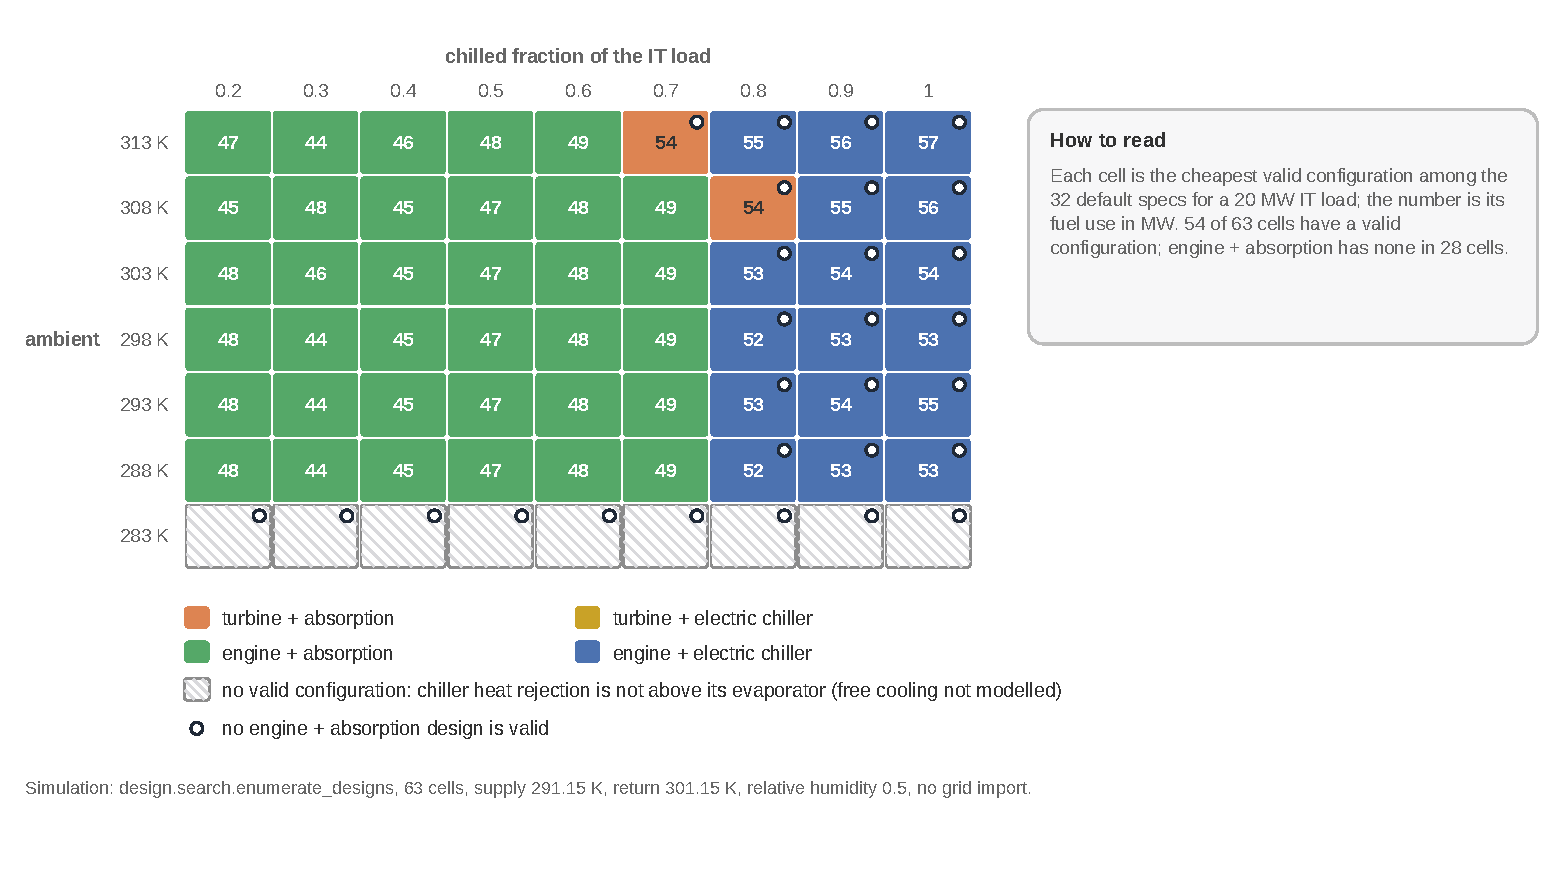
\includegraphics[width=\linewidth]{figures/pdf/fig_design_feasibility.pdf}
\caption{Best configuration family over chilled fraction and ambient temperature for a 20~MW IT load among the \val{feas.n_specs} default specifications (simulation, \val{feas.n_cells} cells). Numbers are fuel use in MW; hatched cells have no valid
configuration in the model; circles mark cells where no engine plus absorption design is valid. Data: \texttt{assets/design\_feasibility.json}.}
\label{fig:fig_design_feasibility}
\end{figure}

\subsubsection{First-law against second-law blame}\label{sec:audit}

A first-law ranking blames the component that dissipates the most energy to the surroundings. In one audited plant (\texttt{aud-0-00000}, a turbine plant with absorption cooling, fuel input \val{aud.ex_fuel_mw}~MW) it blames the heat rejector
\val{aud.ex_rej_id}, which dissipates \val{aud.ex_rej_energy_mw}~MW but destroys \val{aud.ex_rej_ed_mw}~MW of exergy, while exergy is destroyed in the prime mover \val{aud.ex_pm_id} (\val{aud.ex_pm_ed_mw}~MW, with \val{aud.ex_pm_energy_mw}~MW of energy dissipated) and, among the
other components, mostly in \val{aud.ex_top_id} (\val{aud.ex_top_ed_mw}~MW). Over plants, with the prime mover excluded because it was the largest destroyer in every plant, the first-law top choice is the true top destroyer in
\val{aud.fl_hits_id} of \val{aud.n_id} in-distribution plants (random order: \val{aud.rnd_top1_id_pct}\%) and \val{aud.fl_hits_ood} of \val{aud.n_ood} held-out-topology plants (\val{aud.fl_top1_ood_pct}\%, Wilson 95\% interval \val{aud.fl_ci_lo_ood_pct} to \val{aud.fl_ci_hi_ood_pct}\%; random
order \val{aud.rnd_top1_ood_pct}\%). In nDCG@3 the first-law ranking scores \val{aud.ndcg_fl_id} and \val{aud.ndcg_fl_ood} against \val{aud.ndcg_rnd_id} and \val{aud.ndcg_rnd_ood} for random order. The two samples disagree: in-distribution the first-law view is below random order on both metrics, while on the held-out diagrams it is clearly above them, so neither sample supports using energy dissipation as a proxy for exergy destruction. The Audit task therefore hides the destruction and asks the model to compute it; the model result is pending, and \cref{fig:fig_audit_first_vs_second_law} has no model bar.

\begin{figure}[tbp]
\centering
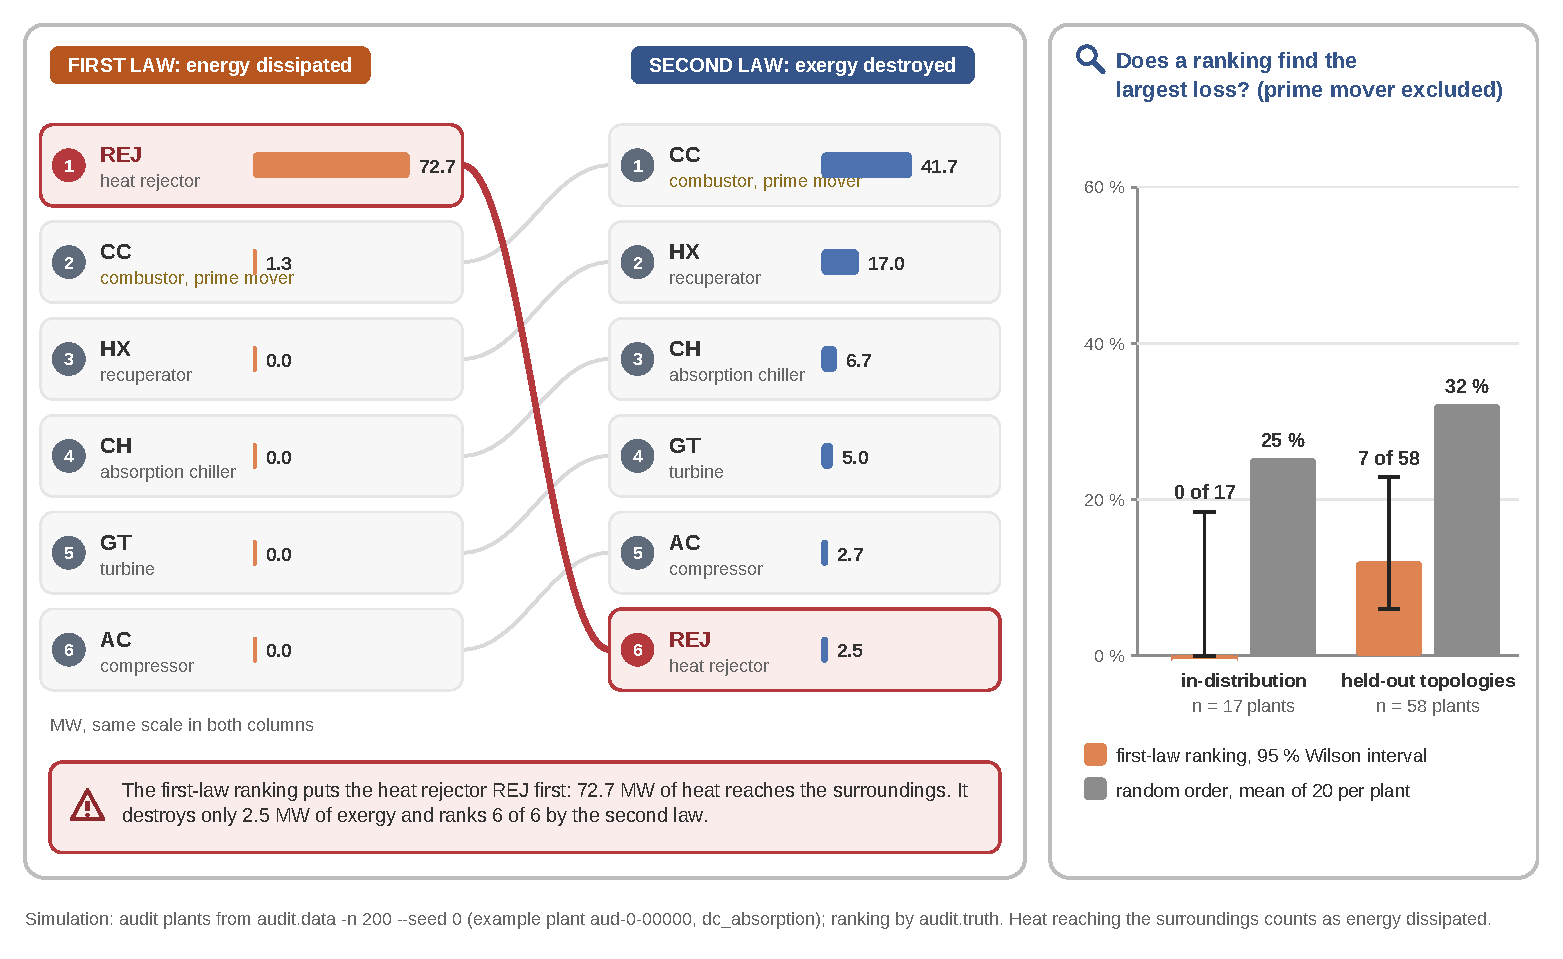
\includegraphics[width=\linewidth]{figures/pdf/fig_audit_first_vs_second_law.pdf}
\caption{First law against second law. Left: energy dissipated to the surroundings and exergy destroyed per component for one plant (simulation, $n=1$). Right: top-1 hit rate of the first-law ranking against random order, prime mover
excluded, on \val{aud.n_id} in-distribution and \val{aud.n_ood} held-out-topology plants (simulation, seed 0); whiskers are 95\% Wilson intervals. Data: \texttt{assets/audit\_first\_vs\_second\_law.json}.}
\label{fig:fig_audit_first_vs_second_law}
\end{figure}

\subsubsection{Symptom coverage of ledger faults}\label{sec:ledger}

For each of \val{led.n} generated ledger rows (\val{led.n_single} with one fault, \val{led.n_double} with two) we ask whether the ledger shows a second-law symptom: a closure residual or a negative exergy destruction.
\Cref{fig:fig_ledger_symptoms} gives the shares per fault type on the \val{led.n_single} single-fault rows. The result has a structure. A closure residual appears when a destruction line is wrong: in \val{led.comp_closure} of
\val{led.comp_rows} rows with a component-line fault. It does not appear for a fault in a stream line or in the constant: in \val{led.stream_closure} of \val{led.stream_rows} such rows, because an error in a stream value $E[x]$ or in $T_0$
enters the destruction lines of its producer and consumer with opposite signs and cancels in the sum (\cref{fig:fig_verifiers}); dropping a work term, by contrast, changes the closure residual by \val{led.demo_drop_work_mw}~MW in the example of the figure.
For those \val{led.stream_rows} rows the only symptom is a negative destruction, visible in \val{led.stream_neg} of them. Overall \val{led.any_pct}\% of the rows show at least one symptom and \val{led.none_pct}\% show none; the two constant faults (\texttt{t0\_celsius}, \texttt{t0\_offset}; \val{led.t0_celsius_n} rows each) show
no symptom at all. Parameter-range checks (V6) see \val{led.range_checks} of these faults, because the faults are in the equations and not in the plant parameters. A model that repairs the ledger therefore has to localize the fault from the text of the lines, not from the checks alone.

\begin{figure}[tbp]
\centering
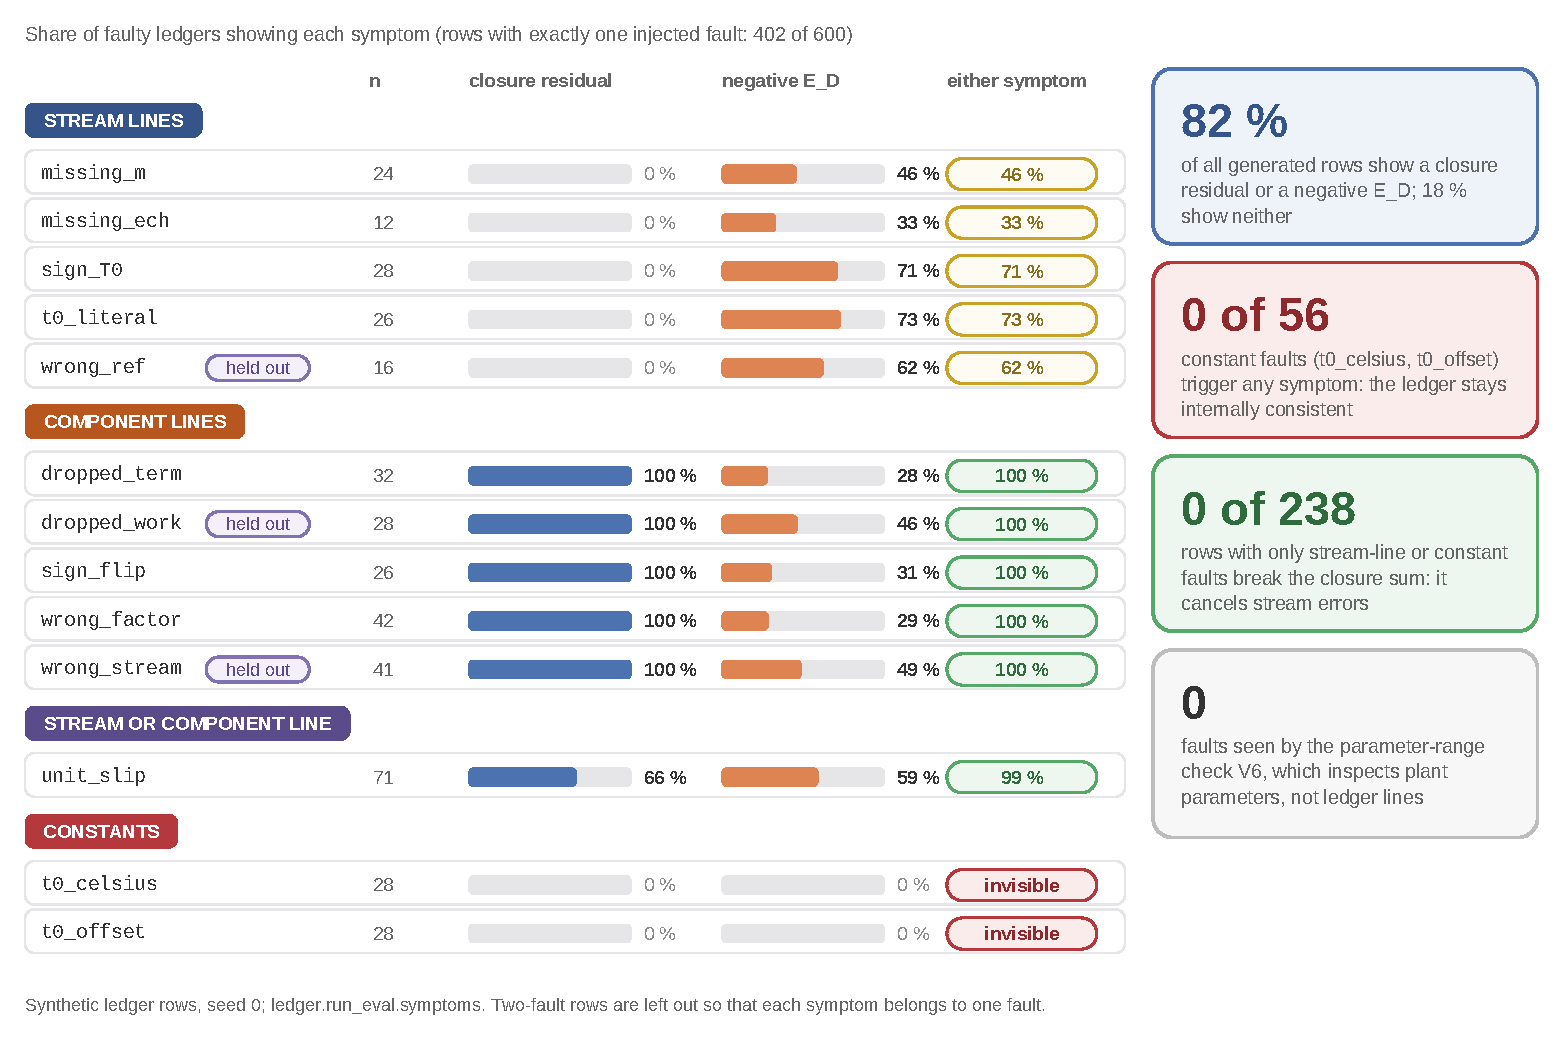
\includegraphics[width=\linewidth]{figures/pdf/fig_ledger_symptoms.pdf}
\caption{Symptoms of injected ledger faults: share of single-fault rows ($n=\val{led.n_single}$ of \val{led.n} generated rows, simulation, seed 0) showing a closure residual, a negative destruction, or either, by fault type and layer.
Stream-line and constant faults never break closure, and two constant faults show no symptom at all; parameter-range checks see none of these faults. Data: \texttt{assets/ledger\_symptoms.json}; the all-rows numbers are in \cref{app:faults}.}
\label{fig:fig_ledger_symptoms}
\end{figure}

\subsection{Current status: datagen and training}\label{sec:datagenstatus}

Datagen is incomplete, and Reza's directive of 2026-11-19 forbids starting SFT, GRPO or any training-based smoke test until every datagen item is built, audited and committed. The deterministic tool corpora currently hold 960 rows, built with \texttt{--limit 120} (240 per task), against a decided size of 4,800 rows (600 plants $\times$ 2 variants $\times$ 4 tasks). The plain A-slice is complete at 1,600 rows ($=\mathrm{round}(4{,}800\times0.3333)$, 400 per task). Only 32 verifier-accepted frontier tool traces exist, all from \texttt{google-gemini-3-8-flash} (40 attempts, five 429 errors, 32 accepted, \$0.842202 total); after sanitizing the provider \texttt{call\_id} wrapper the clean corpus has at most 7,268 tokens per row, all under the 8,192 gate. Luna, haiku, sol, opus, sonnet and gemini-4 traces are planned, not collected. Tiers are equal thirds per task in both training and test data, derived from \texttt{thermo\_agent/synth/tiers.py}, with the remainder to the higher tier. The test set \texttt{heldout\_v2} is frozen before scoring. Consequently there are no results for any SFT, GRPO or evaluation arm: the tables below are skeletons, and every value in \cref{sec:protocol} is planned, not measured.

\subsection{Model results}\label{sec:modelresults}

\Cref{tab:results,tab:comparison} are generated from the result JSON files listed in
\texttt{model\_results\_manifest.json} in the paper assets: one entry per arm, with its model family, mode (Z or H),
tool access and zero-shot flag. The protocol is pre-registered, but no arm has been scored: no trained checkpoint exists and the frontier arms are replays from \texttt{data/kaggle\_datasets/thermo-agent-eval-replays/}. Consequently both tables are skeletons (``pending'') and carry no measured model values, and the teacher acceptance statistics are pending (\cref{tab:corpusstatus}). When
the runs exist we will report all rows for the \texttt{heldout\_v2} test cells, with the intervals and tests of \cref{sec:protocol}; the 214-id \texttt{heldout} remains dev. No planned value is presented as a result.

\begin{table}[tbp]
\centering
\begingroup\scriptsize\setlength{\tabcolsep}{3pt}
\begin{tabular}{@{}p{1.3cm}p{4.4cm}p{1.9cm}p{1.9cm}p{1.9cm}p{1.9cm}@{}}
\toprule
Task & Model (full inference text) & \multicolumn{4}{c}{Metrics (per task; see text)} \\
\midrule
Repair & Qwen3.5-4B base & \todo{pending} & \todo{pending} & \todo{pending} & \todo{pending} \\
 & SFT, ground truth only & \todo{pending} & \todo{pending} & \todo{pending} & \todo{pending} \\
 & SFT, full corpus & \todo{pending} & \todo{pending} & \todo{pending} & \todo{pending} \\
 & SFT + GRPO & \todo{pending} & \todo{pending} & \todo{pending} & \todo{pending} \\
 & Teacher model \todo{name} & \todo{pending} & \todo{pending} & \todo{pending} & \todo{pending} \\
 & Other open model \todo{name} & \todo{pending} & \todo{pending} & \todo{pending} & \todo{pending} \\
\midrule
Design & Qwen3.5-4B base & \todo{pending} & \todo{pending} & \todo{pending} & \todo{pending} \\
 & SFT, ground truth only & \todo{pending} & \todo{pending} & \todo{pending} & \todo{pending} \\
 & SFT, full corpus & \todo{pending} & \todo{pending} & \todo{pending} & \todo{pending} \\
 & SFT + GRPO & \todo{pending} & \todo{pending} & \todo{pending} & \todo{pending} \\
 & Teacher model \todo{name} & \todo{pending} & \todo{pending} & \todo{pending} & \todo{pending} \\
 & Other open model \todo{name} & \todo{pending} & \todo{pending} & \todo{pending} & \todo{pending} \\
\midrule
Audit & Qwen3.5-4B base & \todo{pending} & \todo{pending} & \todo{pending} & \todo{pending} \\
 & SFT, ground truth only & \todo{pending} & \todo{pending} & \todo{pending} & \todo{pending} \\
 & SFT, full corpus & \todo{pending} & \todo{pending} & \todo{pending} & \todo{pending} \\
 & SFT + GRPO & \todo{pending} & \todo{pending} & \todo{pending} & \todo{pending} \\
 & Teacher model \todo{name} & \todo{pending} & \todo{pending} & \todo{pending} & \todo{pending} \\
 & Other open model \todo{name} & \todo{pending} & \todo{pending} & \todo{pending} & \todo{pending} \\
\midrule
Ledger repair & Qwen3.5-4B base & \todo{pending} & \todo{pending} & \todo{pending} & -- \\
 & SFT, ground truth only & \todo{pending} & \todo{pending} & \todo{pending} & -- \\
 & SFT, full corpus & \todo{pending} & \todo{pending} & \todo{pending} & -- \\
 & SFT + GRPO & \todo{pending} & \todo{pending} & \todo{pending} & -- \\
 & Teacher model \todo{name} & \todo{pending} & \todo{pending} & \todo{pending} & -- \\
 & Other open model \todo{name} & \todo{pending} & \todo{pending} & \todo{pending} & -- \\
\bottomrule
\end{tabular}\endgroup

\caption{Model results for the four tasks, generated from \texttt{model\_eval} reports: our checkpoints, frontier models (zero-shot, with inference text, with tools) and other models, with family, inference text and tool access recorded on each row. Metrics per task are listed in \cref{sec:protocol}.}
\label{tab:results}
\end{table}

\begin{table}[tbp]
\centering
\begingroup\scriptsize\setlength{\tabcolsep}{2pt}
\begin{tabular}{@{}p{3.4cm}p{1.8cm}p{2.2cm}p{1.4cm}p{6.2cm}@{}}
\toprule
Model & Family & Inference text & Tools & Metrics by task/split \\
\midrule
frontier\_zero & frontier & none & none & exact\_on\_deducible 0.37, first\_turn\_success 0.63, mean\_solves 1.33 \\
frontier\_zero & frontier & none & none & exact\_on\_deducible 0.33, first\_turn\_success 0.47, mean\_solves 0.77 \\
frontier\_zero & frontier & none & none & exact\_on\_deducible 0.10, first\_turn\_success 0.43, mean\_solves 1.13 \\
frontier\_zero & frontier & none & none & mean\_evals 0.17, mean\_gap\_pct 13.09, valid 0.17 \\
frontier\_zero & frontier & none & none & mean\_evals 0.30, mean\_gap\_pct 24.04, valid 0.20 \\
frontier\_zero & frontier & none & none & mean\_evals 0.07, mean\_gap\_pct 15.26, valid 0.07 \\
frontier\_zero & frontier & none & none & mean\_evals 0.10, mean\_gap\_pct 8.10, valid 0.10 \\
frontier\_zero & frontier & none & none & gain 0.00, pred 0.00, rank 0.09 \\
frontier\_zero & frontier & none & none & gain 0.00, pred 0.00, rank 0.03 \\
frontier\_zero & frontier & none & none & all\_correct 0.00, closure 0.03, exact 0.00 \\
frontier\_zero & frontier & none & none & all\_correct 0.00, closure 0.00, exact 0.02 \\
frontier\_zero & frontier & none & none & all\_correct 0.07, closure 0.07, exact 0.07 \\
frontier\_tools & frontier & none & tools & exact\_on\_deducible 0.37, first\_turn\_success 0.67, mean\_solves 1.07 \\
frontier\_tools & frontier & none & tools & mean\_evals 0.73, mean\_gap\_pct 16.37, valid 0.43 \\
frontier\_tools & frontier & none & tools & gain 0.00, pred 0.02, rank 0.13 \\
frontier\_tools & frontier & none & tools & all\_correct 0.77, closure 0.92, exact 0.77 \\
other\_model & domain-model & none & none & exact\_on\_deducible 0.22, first\_turn\_success 0.27, mean\_solves 0.67 \\
other\_model & domain-model & none & none & exact\_on\_deducible 0.50, first\_turn\_success 0.50, mean\_solves 1.00 \\
other\_model & domain-model & none & none & exact\_on\_deducible 0.17, first\_turn\_success 0.33, mean\_solves 0.73 \\
other\_model & domain-model & none & none & mean\_evals 0.17, mean\_gap\_pct 18.71, valid 0.17 \\
other\_model & domain-model & none & none & mean\_evals 0.30, mean\_gap\_pct 18.89, valid 0.30 \\
other\_model & domain-model & none & none & mean\_evals 0.17, mean\_gap\_pct 13.55, valid 0.17 \\
other\_model & domain-model & none & none & mean\_evals 0.23, mean\_gap\_pct 11.58, valid 0.23 \\
other\_model & domain-model & none & none & gain 0.00, pred 0.00, rank 0.00 \\
other\_model & domain-model & none & none & gain 0.00, pred 0.00, rank 0.00 \\
other\_model & domain-model & none & none & all\_correct 0.23, closure 0.53, exact 0.25 \\
other\_model & domain-model & none & none & all\_correct 0.13, closure 0.17, exact 0.17 \\
other\_model & domain-model & none & none & all\_correct 0.23, closure 0.35, exact 0.28 \\
\bottomrule
\end{tabular}\endgroup

\caption{Comparison axes: model family, inference text and tool access. The paired harness and tool columns isolate how much the physics tools help a frontier model, against the trained 4B and the non-model baselines.}
\label{tab:comparison}
\end{table}

\begin{figure}[tbp]
\centering
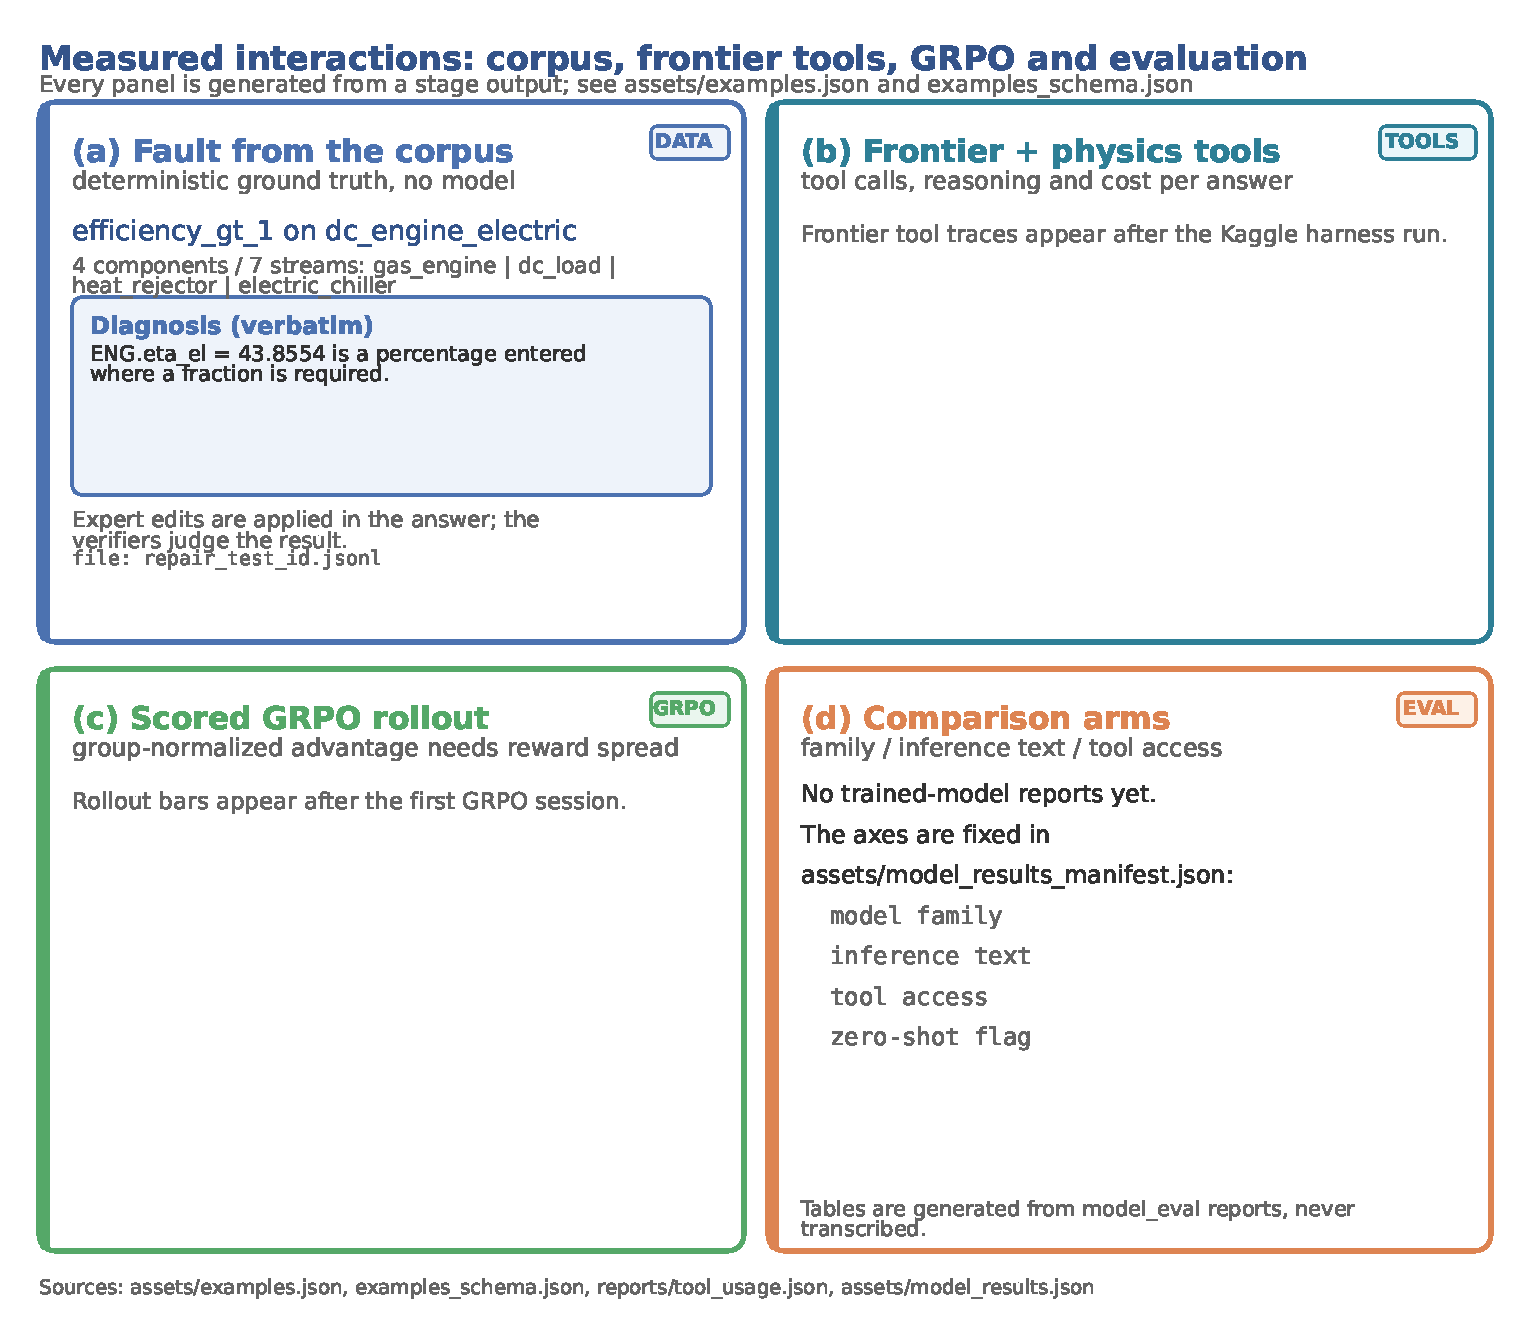
\includegraphics[width=\linewidth]{figures/pdf/fig_trace_walkthrough.pdf}
\caption{Interactions so far: a deterministic fault and its diagnosis, and a frontier model using our physics tools with recorded reasoning and cost (32 accepted traces from one model, replayed). The GRPO rollout and comparison panels are planned, not measured: they fill only after training runs, none of which has occurred. Every available element is copied from a stage output; the schema and selected examples are in \texttt{assets/examples.json} and \texttt{examples\_schema.json}. Regenerated by \texttt{figures\_from\_examples.py}.}
\label{fig:fig_trace_walkthrough}
\end{figure}

\subsection{Ablations}\label{sec:ablations}

\Cref{tab:ablation} lists the planned ablations: the inference text and the tool access on the held-out gas-engine diagrams (RQ2), the training corpus and the number of paraphrase variants per row (RQ7), the memory retrieval against no notes and random notes (RQ7), the reward channels and SFT against GRPO (RQ4), held-out diagram transfer (RQ3), an optional encoder-decoder variant, and ThermoQA accuracy before and after training (RQ6). All results are pending.

\begin{table}[tbp]
\centering
\begingroup\small\renewcommand{\arraystretch}{1.15}
\begin{tabular}{@{}p{4.3cm}p{6.1cm}p{2.9cm}l@{}}
\toprule
Ablation & Arms & Metric & Result \\
\midrule
Inference text on the held-out gas-engine diagrams & none / \texttt{AGENTS.md} / skills / both / both plus memory (base and trained) & success & \todo{pending} \\
Training corpus & ground truth only / plus architecture corpus / plus teacher traces / plus harness and memory text & success on held-out diagrams & \todo{pending} \\
Paraphrase variants per row & 1 / 3 / 20 or more & success on held-out faults & \todo{pending} \\
Memory retrieval & none / retrieved notes / random notes & success and acceptance rate & \todo{pending} \\
Reward channels & full / without site / without minimality / without grounding & success and valid share & \todo{pending} \\
SFT against GRPO from the base model & SFT only / SFT + GRPO / GRPO from base & success & \todo{pending} \\
Encoder-decoder variant (optional) & decoder-only / encoder-decoder & success & \todo{pending} \\
ThermoQA before and after training & base / SFT / SFT + GRPO & accuracy & \todo{pending} \\
\bottomrule
\end{tabular}\endgroup

\caption{Skeleton of the ablations. All results are pending.}
\label{tab:ablation}
\end{table}

\subsection{Reward diagnostics}\label{sec:rewarddiag}

Before any GPU time we asked how often a group of \val{rd.G} completions would have identical rewards, which carry no gradient under group-normalized advantages. The probe uses simulated policies that return the expert answer with probability $1-e$ and a damaged answer otherwise
(\val{rd.repair.groups} groups per task and level, seed 0; no model). At an error rate of 5\% the share of such groups is \val{rd.repair.zv_e5_pct}\% for Repair, \val{rd.design.zv_e5_pct}\% for Design, \val{rd.audit.zv_e5_pct}\% for Audit and \val{rd.ledger.zv_e5_pct}\% for Ledger repair;
at 10\% it is \val{rd.repair.zv_e10_pct}, \val{rd.design.zv_e10_pct}, \val{rd.audit.zv_e10_pct} and \val{rd.ledger.zv_e10_pct}\%; at 30\% it is \val{rd.repair.zv_e30_pct}, \val{rd.design.zv_e30_pct}, \val{rd.audit.zv_e30_pct} and \val{rd.ledger.zv_e30_pct}\%; and at 60\% it is
\val{rd.repair.zv_e60_pct}, \val{rd.design.zv_e60_pct}, \val{rd.audit.zv_e60_pct} and \val{rd.ledger.zv_e60_pct}\%. With the smaller group, equal groups are more frequent: at an error rate of 10\% the shares at a group of 8 are \val{rd8.repair.zv_e10_pct}, \val{rd8.design.zv_e10_pct}, \val{rd8.audit.zv_e10_pct} and \val{rd8.ledger.zv_e10_pct}\%. A task on which the SFT model is already accurate gives GRPO little to learn from, which is the reason for RQ3. A fresh reward evaluation costs
\val{rd.ledger.eval_ms}~ms for the ledger, \val{rd.repair.eval_ms}~ms for Repair, \val{rd.audit.eval_ms}~ms for Audit and \val{rd.design.eval_ms}~ms for Design per completion on the authoring machine (one CPU), so the reward is cheap relative to generation. \Cref{fig:fig_reward_signal} shows the curves.

\begin{figure}[tbp]
\centering
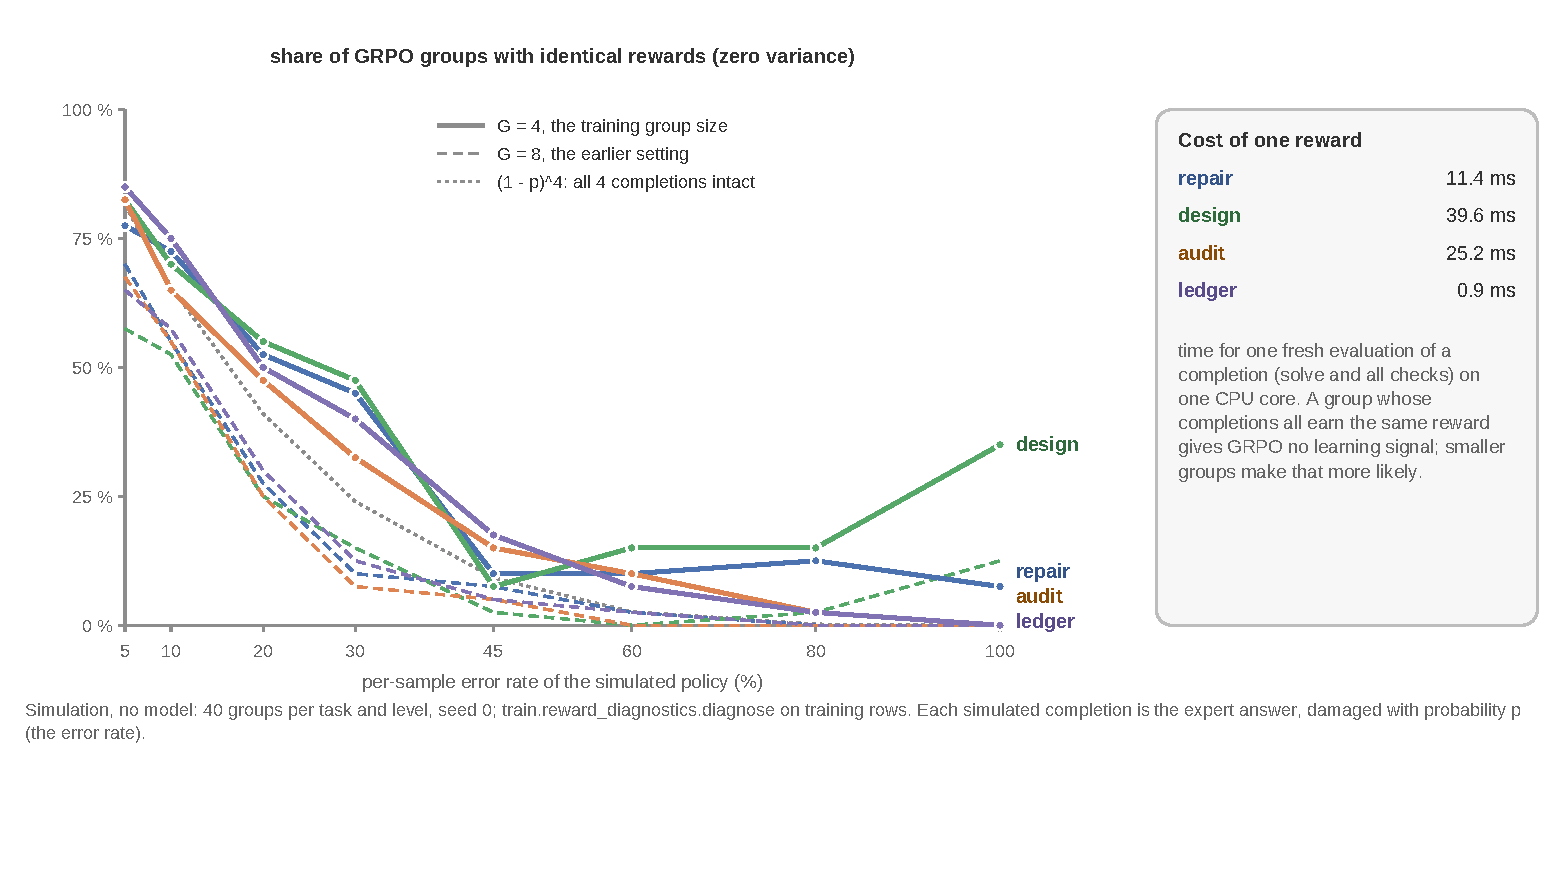
\includegraphics[width=\linewidth]{figures/pdf/fig_reward_signal.pdf}
\caption{Reward signal before any GPU time: share of GRPO groups whose completions all receive the same reward, against the per-sample error rate of a simulated policy, for each task, at the training group size of \val{rd.G} (solid) and at 8 (dashed), with the cost of one reward evaluation (simulated policies on synthetic data, no model; \val{rd.repair.groups} groups per task and level, seed 0). Data: \texttt{assets/reward\_signal.json}.}
\label{fig:fig_reward_signal}
\end{figure}

\subsection{What the remaining claims depend on}\label{sec:status}
The model-independent numbers in this paper are measured and reproducible from the checked-in generators and seeds: the verifier coverage, the baseline search costs, the feasibility and first-law findings, the reward diagnostics, and the data and corpus reports. The trained-model columns of \cref{tab:results,tab:comparison,tab:ablation} are pending, and the following runs are the only evidence that can fill them: the frontier teacher pass on Kaggle, local ingest and grading, the two-stage SFT/GRPO run on two T4 GPUs with resumable checkpoints, and the multi-arm evaluation of \cref{sec:protocol}. None of these runs has been executed. Until those runs exist we make no claim about the relative performance of the 4B model, the frontier arms or the other models, and \texttt{paper/assets/model\_results.json} contains the empty schema rather than numbers. The same rule applies to the cost columns: token prices are recorded when a Kaggle call happens, not estimated here.

\section{Trace and fleet evaluation}\label{sec:trace}

A design chosen at one operating point is operated on a load that varies. Two simulator tools bound the fuel of a design on a load trace, and
neither needs part-load efficiency curves that the model does not have. Both are simulator-only: no trace-based result is a prediction of a fuel bill.

\paragraph{Ideal part-load bound.}
A load trace is split into quantile bins of IT power. The design is evaluated at the median load and coolant temperatures of each bin (and the ambient
temperature when the trace has it), and the fuel is weighted by the time in the bin. The plant is re-sized to every bin, so efficiency does not depend on load: this is ideal
part-load and a lower bound on fuel within the model. Bins in which the design is infeasible are reported by time share and excluded from the energy.

\paragraph{Modular gensets.}
To remove the ideal assumption without inventing efficiency curves, the prime mover is split into $n$ identical units that run at rated output or not at all. The installed capacity is
the largest bin need times a margin, the units online in a bin are the smallest number that covers its need, the plant is solved with that output, and the surplus electricity is curtailed,
so its fuel is wasted. The modularity penalty is the fuel above the ideal part-load bound. Because fuel scales with generation for both prime movers, the penalty depends on the shape of the
load trace and on the unit count and, to first order, not on the technology; parasitic loads that do not scale with generation, such as electric chillers or a heat pump, break the tie slightly.
Not modeled are unit efficiency depending on unit size, minimum run time, start-up and ramp limits, capacity limits of heat-recovery equipment and chillers, and standby units beyond the capacity margin.

\paragraph{A synthetic example.}
\Cref{fig:fig_part_load} applies both tools to a synthetic trace of \val{pl.n_samples} samples (IT load drawn from a normal distribution with a mean of 24~MW and a standard deviation of 5~MW, clipped to 8 to 30~MW, \val{pl.bins} bins, seed 0). It is not Frontier data. For
a turbine plant with absorption cooling and a wet tower at a chilled fraction of 0.5, the ideal bound is \val{pl.turbine.ideal_mwh}~MWh of fuel and a single unit burns \val{pl.turbine.fuel1_mwh}~MWh. The modularity penalty is
\val{pl.turbine.u1_pct}\% for one unit and \val{pl.turbine.u2_pct}\% for two, then \val{pl.turbine.u3_pct}\% for three, \val{pl.turbine.u4_pct}\% for four, \val{pl.turbine.u6_pct}\% for six,
\val{pl.turbine.u8_pct}\% for eight and \val{pl.turbine.u12_pct}\% for twelve units; the values for the engine plant are the same. That the one-unit and two-unit penalties coincide and that the engine and the turbine coincide are properties of this trace and of the
scaling argument above, not findings about the technologies. With one sample trace and one design, the figure shows the size of the effect that a fleet of more units can recover in the model; it makes no statement about real units.

\begin{figure}[tbp]
\centering
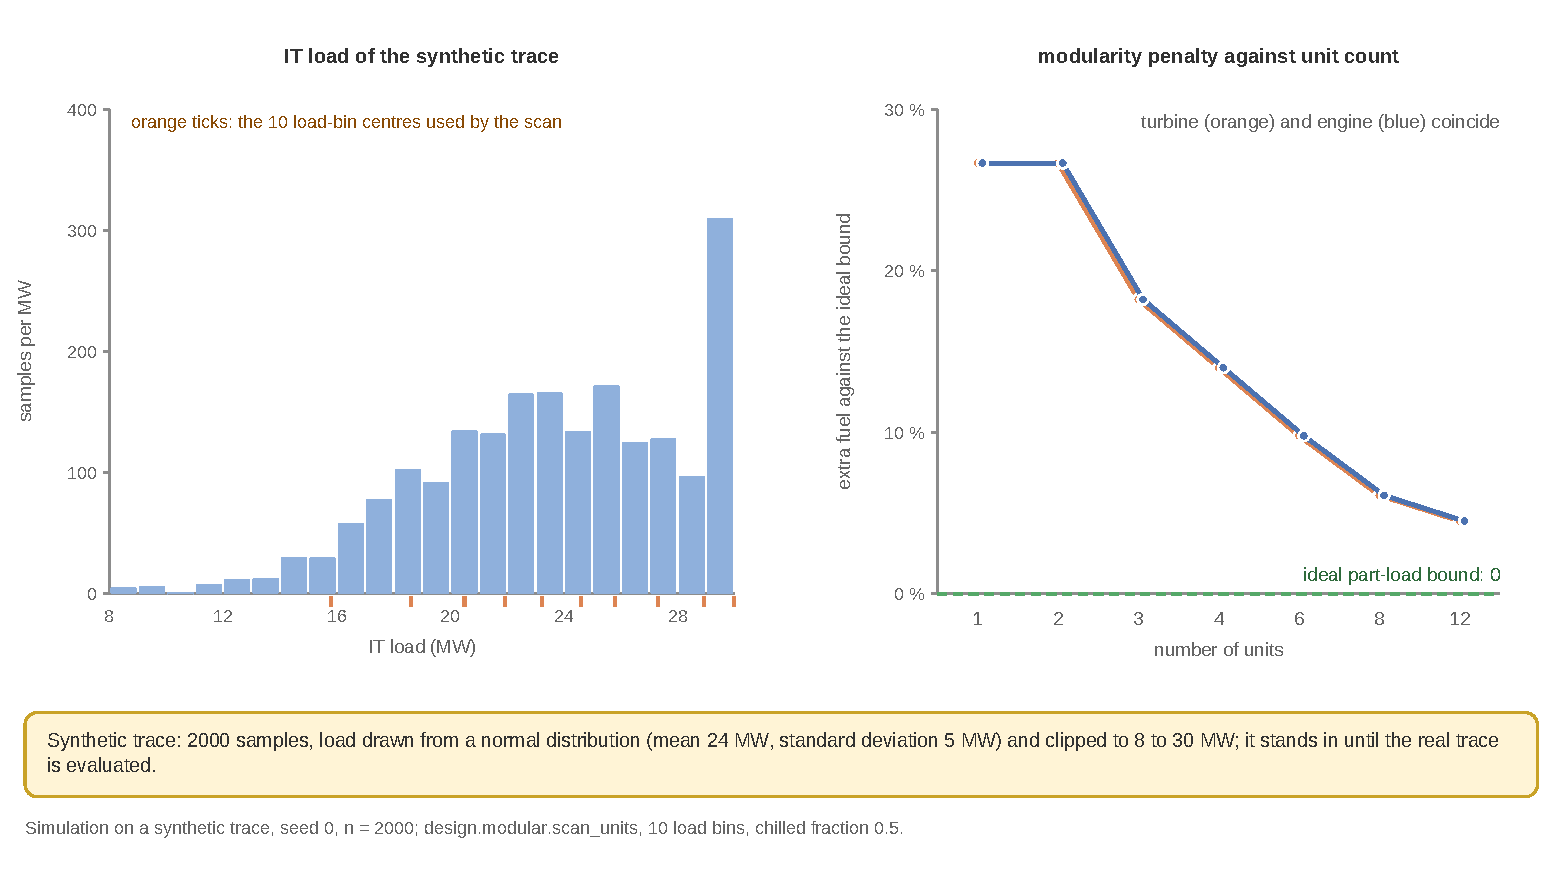
\includegraphics[width=\linewidth]{figures/pdf/fig_part_load.pdf}
\caption{Part-load behavior on a \textbf{synthetic} trace (not Frontier data; \val{pl.n_samples} samples, seed 0, simulation): load histogram with the bin centers used (left) and modularity penalty against the number of
units with the ideal bound at zero (right), for turbine and engine plants with absorption cooling and a wet tower. The trace stays synthetic until the real trace is evaluated. Data: \texttt{assets/part\_load.json}.}
\label{fig:fig_part_load}
\end{figure}

\paragraph{Frontier trace.}
The loader for the published Frontier energy dataset maps explicit columns, and the file has not been downloaded. The evaluation of the catalog and of modular fleets on the measured trace is therefore pending:
\todo{Frontier trace results}.

\section{Limitations}\label{sec:limits}

\paragraph{Assumed technology constants.}
The engine electrical efficiency (0.43) and loss fraction (0.15 by default; 0.10 to 0.20 in the generators), the turbine efficiencies, the chiller reversible-limit fractions and the 0.8 COP cap, the heat-pump approach, the rejector approaches and fan fraction, the ORC fluid
vapor limits, the 333~K stack floor and the fraction of IT heat on the chilled loop are assumed (\cref{tab:constants}). They are not fitted to data, and the Design and Audit outcomes depend on them. In particular, the feasibility limits of \cref{sec:feasibility} follow from these constants.

\paragraph{Heat that is not recovered or modeled.}
Engine jacket and radiation heat is rejected, not recovered. The absorption chiller is a system-level model with a fraction of the reversible COP and a cap, not a LiBr property model.
Water use is an upper bound. At an 18\,$^\circ$C chilled-water supply the chiller sits at its COP cap, so the absorption results are insensitive to $\varepsilon$ there. Free cooling is not modeled, which makes the cold cells of \cref{fig:fig_design_feasibility} infeasible in the model.

\paragraph{Operation.}
There are no real part-load curves, no thermal storage, no dispatch, and no start-up or ramp limits. Trace results are bounds (\cref{sec:trace}), and the modular-fleet penalty depends on the trace shape.

\paragraph{No measured on-site-generation data center.}
Published measurements of a supercomputer set operating points, and nothing in this paper was measured on a data center with on-site generation. The Frontier trace evaluation is pending, and the only trace result is on a synthetic trace. There is no validation against a real plant: the cross-check in \cref{sec:env} is one operating point of one configuration against an independent implementation of the same equations.

\paragraph{Audit.}
The prime mover was the largest destroyer in every plant generated, so the ranking excludes it, and the task is a ranking among the remaining components. The best allowed change is mostly the pressure ratio or the turbine inlet temperature on turbine plants, where a fixed rule recovers \val{audb.rule_gain_id_pct}\% of the best gain when it is valid. The held-out plants (engine and steam-ORC) offer much smaller savings, so the gain channel is small in absolute terms there.

\paragraph{Ledger repair.}
The task is solvable by a rule: a program that rebuilds every line from the topology solves every row by construction. It measures whether a model applies that rule from text and localizes the fault, and it does not measure thermodynamic insight. Of the generated rows, \val{led.none_pct}\% show no second-law symptom, so the checks alone cannot detect them; the model has to find them from the text.

\paragraph{Repair.}
Most Repair faults are caught by parameter-range checks, and the baseline search solves almost all rows. The task is useful for the cost it measures (solver calls), not for difficulty of detection.

\paragraph{Reference and baselines.}
The Design reference is the best design found by enumeration plus a local polish, not a proven optimum, and the enumerate-then-polish curve runs the procedure that defines the reference. The baseline samples are small (\val{des.n_sites} Design sites, \val{aud.n_id} and \val{aud.n_ood} Audit plants, \val{rep.total_n} Repair rows, one example plant for each of the cross-check and the exergy-flow figure), and the intervals are wide where we give them.

\paragraph{Synthetic data.}
All training and evaluation data are sampled by the generators and labeled by the simulator and the verifiers. They are not measurements, and the distribution of plants is the one the generators produce.

\paragraph{Teacher and memory.}
A teacher answer that the tool suite accepts is correct for the checks that the suite has and may still be poor, for example a valid repair that is not the original plant; the checks decide validity and not optimality. Frontier models share habits with the student they teach, which narrows the variety we want, and different models differ in acceptance rate, so the corpus depends on which models were available within the quota and on their recorded prices. The memory is retrieved lexically, and notes mined from rejected or accepted attempts could leak information across splits unless the split of the mined records is controlled. Teacher-authored diagrams are checked by the same tool suite, so they inherit its blind spots: a plant that the verifiers cannot fault is accepted.

\paragraph{Diagram variety.}
The model's understanding of diagrams is tested on held-out diagrams of the catalog. The families in the catalog bound what this tests: a family that is absent cannot be held out, and held-out diagrams of a family that also appears in training test recombination more than novelty (\todo{limits of the final catalog}).

\paragraph{Model results and replay arms.}
At the time of writing no model has been trained or evaluated on a GPU, because none was available locally; the GPU code is reviewed but untested, and the known risks are loading Qwen3.5-4B through the causal-LM class, the TRL argument names, 4-bit loading and merging, and generation-length cutoffs. The runbook records them. Consequently every trained-model statement is pending. Frontier arms are evaluated by replaying saved answers: this gives an identical prompt and verifier for every arm, but it cannot give a frontier model solver feedback after the saved answer, so the frontier-with-tools arm is measured on the traces we collected during generation rather than by re-running the tools at evaluation time. We report this as a limitation of the comparison, not of the environment.

\paragraph{Verifier gaming and software status.}
Verifier gaming is possible. Edits are restricted to existing fields, the site check is in the Repair reward, and the reward functions are tested with junk and mutated answers for robustness (they must not raise and must stay bounded), but this does not exclude gaming by a trained policy. The project has \val{env.n_tests} tests that pass on the CPU; the continuous-integration workflow in the project has never been executed.

\paragraph{Summary of threats and mitigations.}
The main threats are construct validity (a verifier may accept a plant that a physicist would reject), internal validity (the baseline search may define the difficulty of Repair, and the reference design may define the difficulty of Design), external validity (all plants are generated from the same registry and no real plant is measured), and conclusion validity (small samples and many comparisons). We mitigate them, respectively, by publishing the verifier definitions and the accepted/rejected attempts, by reporting the procedures that define the baselines and the reference, by stating explicitly that transfer is between diagrams of the catalog and not to real plants, and by Wilson intervals, paired tests with Holm correction and fixed seeds. These mitigations bound the claims: the results support statements about this environment and its held-out diagrams, not about on-site generation in general.

\section{Conclusion}\label{sec:conclusion}

We described a second-law-verified environment for on-site power, cooling and heat recovery in AI data centers, four task families with structural out-of-distribution splits, and a training recipe that goes from supervised fine-tuning on a verifier-gated, varied corpus (paraphrased traces, a diagram catalog, accepted teacher answers and a failure memory) to GRPO with the
verifiers as the reward. The measured parts are model-independent: non-model baselines that set the cost a model must beat, feasibility limits of the catalog, a first-law ranking that does not locate exergy destruction on a small sample, and a ledger benchmark in which stream-line and constant faults
never break closure. The model results are pending: \todo{headline model result}. We will report them against the frozen protocol of \cref{sec:protocol} and claim only sample efficiency and breadth, and only if the runs support it.


\section*{Data and code availability}
The \sys{} package, the dataset generators and the paper build scripts are in the project
repository. \todo{Add repository, dataset and model-checkpoint links and the licence before
submission.}

\FloatBarrier
\bibliographystyle{plainnat}
\bibliography{refs}

\appendix
\section{Verifier definitions}\label{app:verifiers}

The verifiers in \cref{tab:verifiers} act on a solved plant and, for V7 and V8, on the answer text and the site. They return a boolean and a short detail string. The detail is the feedback given to a model on a retry. A plant is valid when it solves and all hard checks pass. The statements below complement the table.
\begin{itemize}[leftmargin=*,itemsep=1pt]
\item V1 and V2 are residuals per component of the solved balances. V2 is scaled by the sum of the net work, the fuel energy and 1~MW, so that plants of different size share one tolerance.
\item V3a allows a small negative destruction of $10^{-5}$ of the fuel exergy to absorb round-off; V3b is the plant-level closure of \cref{sec:exergy}.
\item V4a is the hard temperature-cross check on every heat exchanger, and V4b the soft practical-pinch check of 1~K.
\item V5 contains four bounds: $\eta_{\mathrm{II}}\in[0,1]$; the power efficiency below the Carnot bound $1-T_0/T_{\max}$; the ORC efficiency below $1-T_{\mathrm{cond}}/T_{\mathrm{hot}}$; and the COP of every chiller and heat pump at or below the reversible COP of its stream temperatures.
\item V6 checks ranges: efficiencies in $(0,1]$, pressure ratio above 1, pressure drops in $[0,0.3]$, temperatures 150 to 2500~K, pressures 1~kPa to 100~MPa, and the direction of pressure change across compressors, pumps and turbines.
\item V7 compares every number with a unit in a reasoning text with solver or plant values within 0.5\% (3\% for predicted Design quantities).
\item V8 checks that the IT load is within 1\%, that electricity balances when grid import is not allowed, that cooling and heat are delivered to at least 99\% of the load, and the water limit.
\end{itemize}

\section{Component parameter registry}\label{app:registry}

\begingroup\scriptsize\setlength{\tabcolsep}{3pt}\renewcommand{\arraystretch}{1.1}
\begin{longtable}{@{}p{3.1cm}p{2.9cm}p{6.6cm}p{2.0cm}@{}}
\caption{Component parameter registry (\texttt{core.components.PARAMS}). ``required'' means no default; other entries are the code default.}\label{tab:params}\\
\toprule
Type & Parameter & Meaning & Default \\
\midrule
\endfirsthead
\toprule
Type & Parameter & Meaning & Default \\
\midrule
\endhead
\texttt{compressor} & \texttt{PR} & pressure ratio (-) & required \\
 & \texttt{eta\_s} & isentropic efficiency (-) & required \\
\texttt{turbine} & \texttt{P\_out} & outlet pressure (Pa) & required \\
 & \texttt{eta\_s} & isentropic efficiency (-) & required \\
\texttt{orc\_turbine} & \texttt{P\_out} & outlet pressure (Pa) & required \\
 & \texttt{eta\_s} & isentropic efficiency (-) & required \\
\texttt{pump} & \texttt{P\_out} & outlet pressure (Pa) & required \\
 & \texttt{eta\_s} & isentropic efficiency (-) & required \\
\texttt{combustor} & \texttt{T\_out} & outlet temperature (K) & required \\
 & \texttt{dp} & pressure-drop fraction (-) & 0 \\
 & \texttt{q\_loss} & heat-loss fraction of fuel LHV (-) & 0 \\
\texttt{recuperator} & \texttt{T\_cold\_out} & cold-side outlet temperature (K) & required \\
 & \texttt{dp\_cold} & cold-side pressure-drop fraction (-) & 0 \\
 & \texttt{dp\_hot} & hot-side pressure-drop fraction (-) & 0 \\
 & \texttt{useful\_heat} & flag: duty counts as delivered heat & 0 \\
\texttt{hrsg} & \texttt{P\_steam} & steam pressure (Pa) & required \\
 & \texttt{dp\_gas} & gas-side pressure-drop fraction (-) & 0 \\
 & \texttt{econ\_approach\_K} & economiser approach (K) & 15 \\
\texttt{orc\_evaporator} & \texttt{pinch\_K} & pinch at the bubble point (K) & 3 \\
 & \texttt{dp\_hot} & hot-side pressure-drop fraction (-) & 0 \\
 & \texttt{flow\_frac} & working-fluid flow between its minimum (0) and maximum (1); used when the flow is not given & required if flow not given \\
 & \texttt{T\_stack\_min} & minimum exhaust outlet temperature (K) & 333.15 \\
 & \texttt{T\_max\_K} & maximum working-fluid vapour temperature (K) & 420 \\
\texttt{condenser} & \texttt{dT\_cw} & cooling-water temperature rise (K) & required \\
\texttt{dc\_load} & \texttt{P\_it} & IT electrical power (W) & required \\
 & \texttt{chilled\_fraction} & share of the heat sent to the chilled loop (-) & 1 \\
 & \texttt{T\_return} & coolant return temperature (K) & required \\
\texttt{absorption\_chiller} & \texttt{T\_chw\_out} & chilled-water outlet temperature (K) & required \\
 & \texttt{T\_gen\_out} & generator outlet temperature (K) & required \\
 & \texttt{dT\_rej} & heat-rejection water temperature rise (K) & required \\
 & \texttt{eps} & fraction of the reversible COP (-) & 0.27 \\
 & \texttt{COP\_max} & first-law COP ceiling (-) & 0.8 \\
\texttt{heat\_pump} & \texttt{T\_sink\_out} & sink outlet temperature (K) & required \\
 & \texttt{eps} & fraction of the Lorenz COP (-) & 0.5 \\
 & \texttt{approach\_K} & evaporator and condenser approach (K) & 5 \\
 & \texttt{Q\_sink} & heat duty to deliver (W); sizes the source cooling & one of Q\_sink or dT\_src \\
 & \texttt{dT\_src} & source-side temperature drop (K) & one of Q\_sink or dT\_src \\
\texttt{electric\_chiller} & \texttt{T\_chw\_out} & chilled-water outlet temperature (K) & required \\
 & \texttt{dT\_rej} & heat-rejection water temperature rise (K) & required \\
 & \texttt{eps} & fraction of the reversible COP (-) & 0.5 \\
 & \texttt{approach\_K} & evaporator and condenser approach (K) & 5 \\
\texttt{heat\_rejector} & \texttt{kind} & 'dry' (dry cooler) or 'wet' (evaporative tower) & dry \\
 & \texttt{approach\_K} & approach to dry-bulb or wet-bulb (K) & required \\
 & \texttt{fan\_frac} & fan electricity as a fraction of heat rejected (-) & 0.015 \\
\texttt{gas\_engine} & \texttt{P\_el} & rated electrical output (W) & required \\
 & \texttt{eta\_el} & electrical efficiency on LHV (-) & required \\
 & \texttt{f\_loss} & jacket and radiation heat, fraction of fuel energy, rejected to ambient (-) & required \\
 & \texttt{air\_excess} & air flow over stoichiometric (-) & 1.8 \\
 & \texttt{P\_exh} & exhaust pressure (Pa) & 110000 \\
\bottomrule
\end{longtable}\endgroup


\section{Fault catalogs}\label{app:faults}

\Cref{tab:faults} lists the fault types of the Repair and Ledger tasks, and \cref{tab:ledgerfaults} gives the symptom shares behind \cref{fig:fig_ledger_symptoms} on the single-fault rows and, for comparison, the share showing either symptom on all rows (which include the \val{led.n_double} two-fault rows; a
stream-line fault combined with a component-line fault breaks closure, so the all-rows closure shares for stream-line faults are not zero).

\begin{table}[tbp]
\centering
\begingroup\small\renewcommand{\arraystretch}{1.12}
\begin{tabular}{@{}p{3.3cm}p{3.0cm}p{7.2cm}l@{}}
\toprule
Task, layer & Fault & Effect & Held out \\
\midrule
Repair & \texttt{efficiency\_gt\_1} & efficiency above 1 & no \\
Repair & \texttt{sign\_flip} & sign of a parameter or flow reversed & yes \\
Repair & \texttt{swapped\_ports} & destinations of two same-fluid streams exchanged & yes \\
Repair & \texttt{unit\_slip} & value off by a factor of $10^{\pm k}$ or a unit offset & no \\
Repair & \texttt{wrong\_fluid} & stream labelled with the wrong fluid & no \\
\midrule
Ledger, stream lines & \texttt{missing\_m} & flow factor missing in a stream line & no \\
Ledger, stream lines & \texttt{missing\_ech} & chemical term missing in a stream line & no \\
Ledger, stream lines & \texttt{sign\_T0} & wrong sign on the $T_0$ term in a stream line & no \\
Ledger, stream lines & \texttt{t0\_literal} & the number 25 in place of $T_0$ & no \\
Ledger, stream lines & \texttt{wrong\_ref} & another stream's reference state in a stream line & yes \\
Ledger, component lines & \texttt{dropped\_term} & a stream dropped from a destruction line & no \\
Ledger, component lines & \texttt{dropped\_work} & work term dropped from a destruction line & yes \\
Ledger, component lines & \texttt{sign\_flip} & flipped sign of a stream term in a destruction line & no \\
Ledger, component lines & \texttt{wrong\_factor} & destruction line scaled by 0.1, 10, 2 or 0.5 & no \\
Ledger, component lines & \texttt{wrong\_stream} & a different stream in a destruction line & yes \\
Ledger, stream or component line & \texttt{unit\_slip} & $/10^3$ for $/10^6$ in a stream line, or a factor $10^{\pm3}$ in a destruction line & no \\
Ledger, constants & \texttt{t0\_celsius} & $T_0$ in Celsius & no \\
Ledger, constants & \texttt{t0\_offset} & $T_0 = 273.15$ & no \\
\bottomrule
\end{tabular}\endgroup

\caption{Fault catalogs. Repair: \val{env.n_repair_faults} parameter-level types; Ledger repair: \val{env.n_ledger_faults} equation-level types in three layers. The held-out Repair faults are sign flip and swapped ports.}
\label{tab:faults}
\end{table}

\begin{table}[tbp]
\centering
\begingroup\small\setlength{\tabcolsep}{4pt}
\begin{tabular}{@{}llrrrrrr@{}}
\toprule
 & & \multicolumn{4}{c}{single-fault rows} & \multicolumn{2}{c}{all rows} \\
\cmidrule(lr){3-6}\cmidrule(lr){7-8}
Layer & Fault & $n$ & closure & neg. $\ED$ & either & $n$ & either \\
\midrule
stream lines & \texttt{missing\_m} & 24 & 0.00 & 0.46 & 0.46 & 46 & 0.70 \\
stream lines & \texttt{missing\_ech} & 12 & 0.00 & 0.33 & 0.33 & 27 & 0.70 \\
stream lines & \texttt{sign\_T0} & 28 & 0.00 & 0.71 & 0.71 & 61 & 0.79 \\
stream lines & \texttt{t0\_literal} & 26 & 0.00 & 0.73 & 0.73 & 59 & 0.86 \\
stream lines & \texttt{wrong\_ref}$^*$ & 16 & 0.00 & 0.62 & 0.62 & 41 & 0.85 \\
component lines & \texttt{dropped\_term} & 32 & 1.00 & 0.28 & 1.00 & 56 & 1.00 \\
component lines & \texttt{dropped\_work}$^*$ & 28 & 1.00 & 0.46 & 1.00 & 48 & 1.00 \\
component lines & \texttt{sign\_flip} & 26 & 1.00 & 0.31 & 1.00 & 60 & 1.00 \\
component lines & \texttt{wrong\_factor} & 42 & 1.00 & 0.29 & 1.00 & 77 & 1.00 \\
component lines & \texttt{wrong\_stream}$^*$ & 41 & 1.00 & 0.49 & 1.00 & 85 & 1.00 \\
stream or component line & \texttt{unit\_slip} & 71 & 0.66 & 0.59 & 0.99 & 134 & 0.98 \\
constants & \texttt{t0\_celsius} & 28 & 0.00 & 0.00 & 0.00 & 54 & 0.35 \\
constants & \texttt{t0\_offset} & 28 & 0.00 & 0.00 & 0.00 & 50 & 0.42 \\
\bottomrule
\end{tabular}\endgroup

\caption{Symptom shares per ledger fault type (simulation, \val{led.n} generated rows, seed 0). Columns are the share of rows showing a closure residual, a negative exergy destruction or either, on single-fault rows
and on all rows. $^*$ marks a held-out fault type. Data: \texttt{assets/ledger\_symptoms.json}.}
\label{tab:ledgerfaults}
\end{table}

\section{Dataset cards}\label{app:datasets}

All four datasets are synthetic: plants and sites are sampled by the code in the repository and labeled by the simulator and the verifiers. They are not measurements, and no measured data is inside them. Files are written per task and split
with a metadata file that records the seed, the settings and the CoolProp and schema versions. The data files are not in the repository; the generators reproduce them. The licence has not been chosen: \todo{licence}.

\paragraph{Ledger.} Repair an equation-level fault in the exergy ledger of a solved plant (\val{env.n_ledger_faults} fault types in three layers; one fault in 70\% of rows, two otherwise). Held out: topologies (steam-ORC and gas-engine plants) and the fault types \texttt{wrong\_stream}, \texttt{dropped\_work}, \texttt{wrong\_ref}.

\paragraph{Repair.} Fix a plant that fails the solver or the verifiers; one fault of \val{env.n_repair_faults} types is injected into a sampled valid plant of one of five topologies, and only faults that the solver or the verifiers detect are kept. Turbine plants are drawn three times as often as the held-out topologies. Exact restoration applies only when the fault is deducible.

\paragraph{Design.} Choose a plant for a sampled site (IT load 5 to 60~MW, log-uniform; chilled fraction 0.3 to 0.95; ambient 283 to 310~K; humidity 0.2 to 0.9; optional heat demand and water limit). The reference is the best of enumeration and a Nelder--Mead polish with at least 60 evaluations (a 15-evaluation polish was measured to be 1.6 to 3.1\% worse). Held out: IT load of 45~MW or more, ambient of 305~K or more, chilled fraction of 0.85 or more.

\paragraph{Audit.} Rank exergy destroyers, propose one allowed change and predict its fuel effect on sampled valid plants, some with ORC bottoming and district heat; only plants in which at least one allowed change saves fuel are kept. Held out: topologies.

\paragraph{Architecture corpus.} Repair rows built from the catalog of \val{corp.n_arch} diagrams (\val{corp.n_dc} data-center plants and the steam plant), with the same fault injectors as the Repair set. Held out: every engine plant and the steam plant. In a seed-0 sample of \val{corp.arch_requested} requested rows, \val{corp.arch_kept} were kept
(train \val{corp.arch_rows.train}, validation \val{corp.arch_rows.val}, in-distribution test \val{corp.arch_rows.test_id}, held-out faults \val{corp.arch_rows.test_ood_fault}, held-out diagrams \val{corp.arch_rows.test_ood_topology}).

\paragraph{Teacher answers, teacher-authored diagrams and memory notes.} Teacher answers are stored with the verdict of the tool suite; accepted answers become rows with the source tag \texttt{frontier}, and every rejected attempt is kept. Teacher-authored plants are stored with the checks they passed or failed, and accepted plants enter the catalog as new diagrams. Memory notes are mined from rejected attempts and carry the task, fault class, diagram, symptom, lesson and fix; the record that a note was mined from is stored so that it can be excluded at retrieval.
Sizes of the final corpus: \todo{rows per source, task and split}.

\begin{table}[tbp]
\centering
\begingroup\small\setlength{\tabcolsep}{4pt}
\begin{tabular}{@{}lrrrrrrrrr@{}}
\toprule
Task & train & val & id & ood fault & ood topology & ood scale & ood climate & ood load & total \\
\midrule
Repair & 6688 & 827 & 784 & 5295 & 279 & -- & -- & -- & 13873 \\
Design & 1768 & 235 & 204 & -- & -- & 460 & 615 & 411 & 3693 \\
Audit & 3299 & 417 & 425 & -- & 141 & -- & -- & -- & 4282 \\
Ledger & 6313 & 828 & 806 & 2875 & 292 & -- & -- & -- & 11114 \\
\bottomrule
\end{tabular}\endgroup

\caption{Rows per split of the small datasets generated for the baselines of this paper (seed 0; Repair 400 rows requested, Audit 200, Ledger 600; Design in 16 chunks of 6 sites, of which \val{des.n_sites} sites were used for the baselines); the training corpus is larger and its sizes are \todo{pending}. Splits for the in-distribution sets are separated by a hash of the example identifier. Data: \texttt{assets/splits.json}.}
\label{tab:datasets}
\end{table}

\section{Reward formulas}\label{app:rewards}

With weights in brackets (\cref{tab:tasks}). \textbf{Repair} [0.5, 2, 1, 1, 0.5, 0.5]: format; validity (1 if the plant solves and passes all hard checks, else $0.5\times$ the fraction of checks passed); site requirements; exact restoration when the fault is deducible; minimality $1/(1+\text{extra edits beyond the minimum})$; grounding.
\textbf{Design} [0.5, 2, 2, 0.5]: format; validity (1 valid, 0.2 built but invalid); quality $1-(F-F_{\mathrm{ref}})/(0.1\,F_{\mathrm{ref}})$ clipped to $[0,1.05]$; grounding of predicted numbers.
\textbf{Audit} [0.5, 1.5, 1, 2, 1, 0.5]: format; nDCG@3 of the ranking with the prime mover removed; validity of the change; gain (saved fuel over the best allowed saving, clipped to $[0,1.05]$); prediction $1-|\hat y-y|/\max(|y|,0.002\,F)$; grounding.
\textbf{Ledger} [0.5, 1, 0.5, 2.5, 0.5, 0.5]: format; closure (1 when $|\text{residual}|\le10^{-6}$ of fuel exergy, falling to 0 at 1\%); share of components with $\ED\ge0$; exactness (faulty lines that now evaluate to the true value minus correct lines now broken, over faulty lines); minimality $1/(1+\text{extra lines})$ once everything is correct; diagnosis numbers in MW must appear in the prompt.

\section{Hyperparameters and compute}\label{app:compute}

The training settings are in \cref{tab:training}. SFT, merge and GRPO have never been run on a GPU. The training target is a Kaggle notebook with two T4 GPUs (16~GB each): two data-parallel ranks, fp16 LoRA, no 4-bit weights, with an estimated 11 to 12~GB per GPU for SFT and about 11~GB for GRPO (estimates, not measured). The frontier teacher is not self-hosted: it runs through Kaggle's model access and needs no GPU of ours. Larger GPUs (bf16, 24 to 48~GB) use the same scripts with other settings; Kaggle TPUs are not supported by these scripts; and a laptop with a 6~GB GPU is used for data generation, tests, non-model baselines and smoke checks with a locally served model, never for training.
GPU hours, wall-clock times and costs of the runs: \todo{pending}.
Everything in \cref{sec:baselines,sec:findings,sec:trace} was computed on one CPU core with \val{env.n_tests} passing tests (\val{env.tests_minutes}~minutes) and library versions CoolProp~\val{env.ver.CoolProp}, NumPy~\val{env.ver.numpy}, SciPy~\val{env.ver.scipy}, pydantic~\val{env.ver.pydantic}, pandas~\val{env.ver.pandas} and Python~\val{env.ver.python}.

\section{Harness text}\label{app:harness}

The harness file \texttt{AGENTS.md} has \val{har.agents_lines} lines (\val{har.agents_chars} characters), whose sections are listed in \cref{tab:agents}. The skills are listed in \cref{tab:skills} and the modes in \cref{tab:modes}. The memory layer is separate from the four modes (\cref{sec:harness}). The held-out component is the gas engine, with \val{har.engine_n_ports} ports; it appears in the held-out-topology splits, with \val{har.heldout_repair_engine_rows} of \val{har.heldout_repair_rows} Repair rows and \val{har.heldout_audit_engine_rows} of \val{har.heldout_audit_rows} Audit rows in those splits involving an engine plant (the others use the steam-ORC plant).

\begin{table}[tbp]
\centering
\begingroup\small\renewcommand{\arraystretch}{1.12}\begin{tabular}{@{}p{3.0cm}rp{9.0cm}@{}}\toprule
Section & lines excerpted & First excerpted line \\
\midrule
Conventions & 2 & \texttt{- SI units: K, Pa, W, kg/s. Efficiencies, second-law fractions (eps) and pressure-drop fractions (dp*) are fractions, never per...} \\
What the verifiers check & 1 & \texttt{V1 mass balance, V2 energy balance, V3 exergy: closure and no negative exergy destruction in any component, V4 no temperature c...} \\
Reading a solver error & 2 & \texttt{- E\_PROP\_RANGE: a value is non-positive, a unit slip, or outside the property data (a pressure of 20 Pa, a temperature of 1226 ...} \\
Answer formats & 2 & \texttt{- Repair: <diagnosis> citing only numbers shown, then <edits> with lines SET <component>.<param> = <number>, SET @<stream>.<fie...} \\
Habits & 2 & \texttt{1. Find which stream or parameter the error or failing check points at before editing anything.} \\
Components & 2 & \texttt{- compressor: ports in, out; params PR, eta\_s} \\
\bottomrule
\end{tabular}\endgroup

\caption{Sections of \texttt{AGENTS.md} with the number of lines excerpted into the harness data and the first line of each (truncated). Data: \texttt{assets/harness.json}.}
\label{tab:agents}
\end{table}

\begin{table}[tbp]
\centering
\begingroup\small\renewcommand{\arraystretch}{1.12}
\begin{tabular}{@{}ll@{}}
\toprule
Skill & Components covered \\
\midrule
\texttt{absorption-chiller} & \texttt{absorption\_chiller} \\
\texttt{design-catalog} & task-level \\
\texttt{exergy-audit} & task-level \\
\texttt{exergy-ledger} & task-level \\
\texttt{gas-engine} & \texttt{gas\_engine} \\
\texttt{heat-pump-district-heat} & \texttt{heat\_pump}, \texttt{recuperator} \\
\texttt{heat-rejector} & \texttt{heat\_rejector} \\
\texttt{orc-bottoming} & \texttt{orc\_evaporator}, \texttt{orc\_turbine}, \texttt{pump}, \texttt{condenser} \\
\bottomrule
\end{tabular}\endgroup

\caption{The \val{env.n_skills} skills and the components each covers; port and parameter sections of component skills are generated from the registry.}
\label{tab:skills}
\end{table}

\begin{table}[tbp]
\centering
\begingroup\small\renewcommand{\arraystretch}{1.12}
\begin{tabular}{@{}lll@{}}
\toprule
Mode & \texttt{AGENTS.md} in prompt & Skill bodies in prompt \\
\midrule
\texttt{none} & no & no \\
\texttt{agents} & yes & no \\
\texttt{skills} & no & yes \\
\texttt{agents+skills} & yes & yes \\
\bottomrule
\end{tabular}\endgroup

\caption{Harness modes. In skill modes the bodies of the selected skills are appended to the system message.}
\label{tab:modes}
\end{table}

\section{Runbook summary and reproducibility checklist}\label{app:runbook}

The steps below are in the project runbook, and every number in this paper from a baseline or a simulator study is regenerated by \texttt{tools/generate\_paper\_assets.py} with the commands recorded in \texttt{assets\_summary.json}.
\begin{enumerate}[leftmargin=*,itemsep=1pt]
\item Install the locked requirements and the package; check that the generated harness text is in sync (the harness builder has a check mode) and that all \val{env.n_tests} tests pass.
\item Generate the data on the CPU: Repair, Audit, Design (with at least 60 evaluations for the reference), Ledger and the architecture corpus, with fixed seeds, and mine the first memory notes; run the data report, whose \texttt{problems} field must be empty.
\item Run the non-model baselines (one evaluation module per task) and the reward diagnostics.
\item Export the prompts, run them against the frontier models through Kaggle's model access, validate the completions locally (resumable; every attempt is logged), check the acceptance rates on a small limit, then scale up and rebuild the combined corpus.
\item Evaluate the base model with and without the harness; check the chat template with the SFT print-sample; run SFT (smoke test, then full) and GRPO per task from the merged model with the two-rank launcher of the repository, and evaluate each stage.
\item Run the ablations, the ThermoQA before and after, the Design anytime protocol and the paired comparisons (\texttt{eval.compare}); evaluate the Frontier trace when the file is available, giving the sampling interval explicitly.
\end{enumerate}
Checklist: seeds are fixed (seed 0 for all generated data in this paper); sample sizes are stated at every number; pending items are red \texttt{\textbackslash todo} markers; no figure shows a trained-model result. The last steps are pending \todo{pending}.


\end{document}
